\documentclass[11pt,letterpaper,twoside]{report}

\usepackage{blindtext}



% This package allows me to put the proper entries in the TOC for chapters and
% appendices.
\usepackage{apptools}

% Layout
\usepackage{geometry}
\usepackage{setspace}
\usepackage{titlesec}
\titleformat*{\section}{\normalfont\Large\bfseries\singlespacing}
\titleformat*{\subsection}{\normalfont\large\bfseries\singlespacing}
\titleformat*{\subsubsection}{\normalfont\normalsize\bfseries\singlespacing}

\usepackage{tocloft}
% Using {2} instead of {1} would list subfigures.  I don't think the graduate
% school would like that.
\setcounter{lofdepth}{1}
% Indent the first paragraph of a section, per graduate school's new
% requirements.
\usepackage{indentfirst}
% Don't indent footnotes, per graduate school's new requirements.
\usepackage[hang,flushmargin]{footmisc}

% Citation style
\usepackage[square,comma,sort&compress]{natbib}
%\usepackage{apalike}

%\usepackage[T1]{fontenc}

% Allows for more sophisticated manipulation of length variables.
\usepackage{calc}

% include citations inline
\usepackage{bibentry}
\nobibliography*

% Figures
% Bjoern used subfigure, but I use subcaption.  Either could be used, but it
% might be necessary to tweak arguments to other packages for compatibility.
%\usepackage{subfigure}
\usepackage[labelformat=simple,list=on]{subcaption}
%\renewcommand\thesubfigure{(\alph{subfigure})}
%\captionsetup{belowskip=4pt}
\usepackage{graphicx}
\graphicspath{{figs/}}
%\DeclareGraphicsExtensions{.pdf,.jpeg,.png}
\usepackage{booktabs}
\usepackage{multicol}
\usepackage{listings}
%\usepackage{subfig}

% Multi-row table cells
\usepackage{multirow}

% Enumeration
% \usepackage{enumitem}


\usepackage{algorithm} 
%\floatname{algorithm}{Listing}
\usepackage[noend]{algpseudocode} 
\usepackage{verbatim}

% Math
\usepackage{amsthm}
\usepackage{amsmath}
\usepackage{amssymb}
\usepackage{mathtools}
\usepackage{thmtools}
\usepackage{bm}
% Restatable theorems.  I used this to be able to repeat a theorem in the
% appendix with the same numbering as in the dissertation.
\usepackage{thm-restate}

% Tikz
\usepackage{tikz}
\usepackage{fontawesome5}
\usetikzlibrary{arrows, arrows.meta, decorations.pathreplacing, patterns, automata, positioning, fit, shapes, backgrounds, calc, patterns.meta}

% Macros
\usepackage{ifthen} % used for, e.g., \job macro with optional job number

% Algorithms.  A different algorithms package should work well, but these
% settings are the best for algorithm2e.

\usepackage{algorithm}
\usepackage{algpseudocode}

% % \usepackage[]{algorithm2e}
% \usepackage[algo2e,lined,boxed,algochapter]{algorithm2e}
% \setlength{\algomargin}{1.7em}
% \SetAlgoSkip{}
% \SetAlCapSkip{2ex}
% \SetAlCapSty{textnormal}


%\makeatletter
%\renewcommand{\ALG@name}{Listing}
%\makeatother

% Typography
% Bjoern used \usepackage{times}, which doesn't affect math mode.  This one is
% better because it does.
\usepackage{mathptmx}
% less curvy mathcal symbols.
% http://tex.stackexchange.com/questions/109968/my-mathcalu-turns-out-to-be-curvy-different-than-default
\DeclareMathAlphabet{\mathcal}{OMS}{cmsy}{m}{n}
\usepackage{microtype}
\usepackage{textcomp}

% Macro support
\usepackage{xspace}
\xspaceaddexceptions{]\}$)$}

% Commenting
\usepackage{comment}

% % Fixed-width font for listings (https://tex.stackexchange.com/questions/451339/sans-serif-font-in-text-monospace-serif-within-algorithm)
\makeatletter
\algrenewcommand\ALG@beginalgorithmic{\ttfamily}
\makeatother


% Fixes
\usepackage{makerobust}

\usepackage{url}
\usepackage{breakurl}
\def\UrlBreaks{\do\/\do-}



% For weird tables:
% \usepackage{tabularx}
% \usepackage{threeparttable}
\usepackage{multirow}

% \def\chaptertobuild{conclusion/main}\chapter[~~~~~~~~~~~~Conclusion]{Conclusion}
\label{ch:conclusion}

Despite the prevalence of companies testing their autonomous vehicles on the road, there is no consensus on end-to-end requirements for AV certification and testing.
%
This dissertation aimed to address some critical aspects of this mission, particularly focusing on the formulation of the traffic rules requirements and its compliance testing for AVs.
%
In Chapter 1, we presented our thesis as follows:
\begin{quote}
\textit{
    Autonomous vehicles are required to have interpretable behavior. Formal logic can be used to give an intuitive but precise model of the traffic rules requirement. The model can be leveraged for verification and validation, namely in test-case generation and coverage arguments.
}
\end{quote}
The key contributions of this work in support of the above thesis can be summarized as follows:

    \textbf{Formulation of Traffic Rules in Formal Logic}.
    We developed a comprehensive framework for representing traffic rules in first-order logic and answer-set programming.
    %
    This formalization allows incremental modeling of the traffic rules, which is a feature of non-monotonic reasoning.
    %
    Furthermore, it allows automated reasoning on traffic rules using off-the-shelf solvers.
    %
    We also developed an application of this framework, namely generating traffic-rules-compliant traffic in simulation.

    \textbf{Development of Complexity-Driven Test-case Generation}.  
    First, we proposed a formal definition of test-case complexity.
    %
    Our definition is objective in the sense that it does not rely on subjective assessments of what features may challenge an AV to pass a test-case.
    %
    Instead, we rely directly and only on the pass-fail criteria.
    %
    Second, we propose an algorithm to generate more-complex test-case scenarios.
    %
    Our technique can handle pass-fail criteria that regard the traffic rules and right-of-way at an intersection, in addition to goal-reach and collision avoidance.
    %
    Similar to~\cite{Karimi.2020}, we expect the traffic rules to be provided in a logic program (more precisely an Answer Set Program \cite{Lifschitz.2010}).
    %
    Our algorithm takes as input the geometry of the traffic intersection, traffic rules to be followed at the intersection, and the routes of the vehicles and generates several test-case scenarios with increasing order of complexity.
    %
    Our algorithm gives full coverage over some subspaces of the possible test-cases: after the set of lane events of two cars are fixed, there are only a finite number of relative temporal order of these events that may result in a more complex test-case, and our algorithm uses an ASP solver to do an exhaustive search over this subspace.
    %
    Third, we generate test-cases for a four-way stop, a T-intersection, and an uncontrolled Y-intersection.
    %
    Then we execute these test-cases to test CARLA's autopilot and autopilot-plus-RSS in the CARLA simulator.
    %
    We incrementally increased the complexity of test-cases and discovered instances where the CARLA autopilot failed test-cases by violating a traffic rule or colliding with a non-ego vehicle.
    %
    Also we observed that restricting the behavior of CARLA's autopilot with RSS improved its rate of success, but did not guarantee passing a test-case.

    \textbf{Comparison of techniques for Coverage-Driven Test-case Scenario Generation}.
    First, we proposed a new predicate coverage metric for AV behaviors that is explainable and can express several important aspects of their functional correctness.
    % 
    Second, we proposed coverage driven fuzzing algorithms for improving the predicate coverage of AV implementations at intersections.
    % 
    We demonstrated that fuzzing techniques that are driven by predicate coverage outperform code coverage and random fuzzing.
    % 
    Third, we investigated what type of coverage metrics and power schedules are more suitable for generating a diverse set of traffic scenarios.
    % 
    Finally, we investigated if test scenarios generated for one implementation can be used for other implementations and report our findings.
    % 
    We evaluated the algorithms in a robust manner by generating test cases for four different publicly available AV implementations on the CARLA platform.





%----------------------------------------
\section{Future Work}

This dissertation lays the foundation for several directions for future research and development:
%-----------------------------------
\subsection{Coverage-driven Fuzzing}
In this dissertation we examined the effectiveness of fuzzing for coverage-driven test-case generation and got encouraging results.
%
We propose a few more research questions in this direction.

%----------------------
\textbf{Nonego Models.}
The first question is, what nonego models are suitable for the fuzzing framework?
%
In this dissertation we used BSplines for representing trajectories, for their \emph{local control property} which allows mutation-based local search, their compact representation using the control points, and their richness which subsumes the class of kinematically/dynamically feasible trajectories.
%
An interesting alternative is representation using Behavior Trees.
%
This representation is widely used in robotics and video games since it allows modeling reactive agents, it is modular and interpretable, and allows using other models as building blocks.
%
The modularity of behavior trees is helpful for fuzzing as it allows structure-aware mutation operators.
%
Another curious alternative is data-driven models, e.g. generative models in machine learning.
%
Having such models, we can investigate the question of whether fuzzing the generative model would help with predicate coverage, compared to the baseline of randomly sampling from the generative model.
%
On possible challenge here is that the scenario encodings in generative models are usually unstructured, represented simply as a vector of numbers, which prohibits using structure-aware mutation.

%-----------------------------------------
\textbf{Transfer of Coverage between AVs.}
In this dissertation we observed an asymmetric transfer of coverage between the rule-based agents and the learning-based agent.
%
This encourages further investigations, which would require integrating more machine-learning-based AV agents into our CARLA platform.
%
Another interesting question is, whether the transfer of coverage depends on the nonego models (BSplines, behavior trees, etc.)



%-----------------------------------
\subsection{Complexity-driven Testing}
In this dissertation we proposed a formal notion of complexity, capturing the difficulty level of passing a test-case.
%
We believe that the formal definition is powerful in the sense that it directly captures the informal notion of test-case difficulty level.
%
However, this generality comes with the representation and computation challenges.
%
In our work, we studied some special cases where we can compute the complexity partial order exactly.
% 
However, in many applications we rather have more flexibility in which special cases we can work with, at the expense of tolerating some error in computing the complexity relation.
%
To give an analogy, we may prefer to work with polynomials for their nice analytical and computational properties at the expense of tolerating the error caused by approximating the target functions with polynomials.
%
The key here is that we want the error to be bounded, because if there is no bound then `approximation' looses its meaning.
%
This setup leads to several research questions.
%
For example, how can we quantify complexity and compute it?
%
In particular, in what cases the complexity partial order is a finite order?
%
In what cases the partial order is countably infinite?



%-------------------
\section{Conclusion}

In conclusion, this dissertation makes  strides towards the certification of autonomous vehicles by laying down a foundation for formulating the traffic rules requirements and developing appropriate testing methodologies.
%
The proposed framework enhances coverage of the requirements, contributing to the broader goal of certifying AVs for integration into our transportation systems.
%
As the field continues to evolve, the insights and tools developed in this research will serve as valuable resources for researchers, industry stakeholders, and regulatory bodies, driving further advancements in AV technology and certification.

% Support for building only one chapter at a time.
% \ifdefined\chaptertobuild
%     \includeonly{\chaptertobuild}
%     \newcommand*\updatechaptername{}
% \fi

% For rules:
% There may be a more elegant way to do this.
% Note that you must have the following line before loading enumitem, otherwise
% things break in weird, hard-to-debug ways.
\let\labelindent\relax
\usepackage{enumitem}
\newenvironment{rules}[1]
{\begin{enumerate}[label=\textbf{#1\arabic*}, ref=#1\arabic*, itemsep=1pt,
topsep=2pt]}
{\end{enumerate}}

\newenvironment{rrules}[2]
{\begin{enumerate}[label=\textbf{#1\arabic*}, ref=#1\arabic*, start=#2,
itemsep=1pt, topsep=2pt]}
{\end{enumerate}}

\DeclareMathOperator*{\argmin}{arg\,min}

\hyphenation{Off-loading}
\hyphenation{Dangerous}
\hyphenation{Interface}

% PDF links
\usepackage[hidelinks,pdfauthor={Alyssa Byrnes}, pdfpagemode={UseOutlines}]{hyperref} % backref=page

% PDF version
\pdfminorversion=7 % doesn't seem to work

%Todo notes
\usepackage[colorinlistoftodos]{todonotes}

\usepackage{pdfcomment}


\input{common/layout}
\input{common/macros}



% https://www.overleaf.com/learn/latex/Questions/What_does_%22%5Cpdfendlink_ended_up_in_different_nesting_level_than_%5Cpdfstartlink%22_mean%3F
\begin{document}

% front matter pages use 2in top margin
\newgeometry{left=1in,top=2in,right=1in,bottom=1in,nohead}
\pagenumbering{roman}

%1. Title Page
\begin{titlepage}
\begin{center}

% 1. The title of the thesis/dissertation, centered 2" below the top of the page

\vspace{2in}
\begin{singlespace}
    \MakeUppercase{Towards Certification of Autonomous Cars: formulating the requirements and testing the compliance}\\ %ALL CAPS
\end{singlespace}


% 2. Your name, centered 1" below the title.
\vspace{61pt} % 1 in = 72pt, 11pt for the line with text
Abolfazl Karimi
\end{center}


%3. The following statement, within the full mar- gins, 1" below your name:
%"A dissertation [or thesis] submitted to the faculty at the University of North Carolina at Chapel Hill in partial fulfillment of the requirements for the degree of	in the Department [or School or Curriculum] of      ."

\vspace{39pt}
\begin{singlespace}
\noindent
\begin{center}
A dissertation submitted to the faculty at the University of North Carolina at Chapel Hill
in partial fulfillment of the requirements for the degree of Doctor of Philosophy in
the Department of Computer Science.
\end{center}
\end{singlespace}


%4. On the lower half of the page, centered, the words "Chapel Hill"
%and one line below that, the year in which your committee approves
%the completed thesis/dissertation.
\vspace{39pt}
\begin{center}
\begin{singlespace}
Chapel Hill\\
2024
\end{singlespace}
\end{center}

%5. On the right-hand side of the page, "Approved by," followed by lines for the
%signatures of the adviser and four (two for thesis) readers. List

\vspace{39pt}
\begin{flushright}
\begin{minipage}[t]{1.8333 in}
Approved by:\\
Parasara Sridhar Duggirala\\
Ron Alterovitz\\
Samarjit Chakraborty\\
Missy Cummings\\
Jonathan DeCastro\\
\end{minipage}
\end{flushright}

\end{titlepage}


\newgeometry{left=1in,top=8.47in,right=1in,bottom=1in,nohead}
%2. Copyright Page (optional)
%If you wish to copyright your thesis, you must include a copyright page with the following information single-spaced and centered on the bottom half of the page:
%© Year 
%Full Name (exactly as it appears on the title page) 
%ALL RIGHTS RESERVED
%This page should immediately follow the title page, and should bear the lower case Roman numeral: ii.

\begin{center}
\begin{singlespace}
\copyright 2024\\
Abolfazl Karimi\\
ALL RIGHTS RESERVED
\end{singlespace}
\end{center}

\clearpage


\newgeometry{left=1in,top=2in,right=1in,bottom=1in,nohead}
% Normal pages from here on out; TOC title takes care of 2in requirement.
\restoregeometry
%3. Abstract
%The word "Abstract" should be centered 2? below the top of the page. 
%Skip one line, then center your name followed by the title of the 
%thesis/dissertation. Use as many lines as necessary. Centered below the 
%title include the phrase, in parentheses, "(Under the direction of  
%_________)" and include the name(s) of the dissertation advisor(s).
%Skip one line and begin the content of the abstract. It should be 
%double-spaced and conform to margin guidelines. An abstract should not 
%exceed 150 words for a thesis and 350 words for a dissertation. The 
%latter is a requirement of both the Graduate School and UMI's 
%Dissertation Abstracts International.
%Because your dissertation abstract will be published, please prepare and 
%proofread it carefully. Print all symbols and foreign words clearly and 
%accurately to avoid errors or delays. Make sure that the title given at 
%the top of the abstract has the same wording as the title shown on your 
%title page. Avoid mathematical formulas, diagrams, and other 
%illustrative materials, and only offer the briefest possible description 
%of your thesis/dissertation and a concise summary of its conclusions. Do 
%not include lengthy explanations and opinions.
%The abstract should bear the lower case Roman number ii (if you did not 
%include a copyright page) or iii (if you include a copyright page).

\begin{center}
\vspace*{52pt}
% Don't use \Large
{\textbf{ABSTRACT}}
\vspace{11pt}

\begin{singlespace}
    Abolfazl Karimi: Simulation-based Testing of the Traffic Rules Requirements for Autonomous Vehicles at Intersections\\
(Under the direction of Parasara Sridhar Duggirala)
\end{singlespace}
\end{center}

% Flow:
% - context and problem
% - briefly highlight contributions


%---------------------------------------------------------

To successfully integrate autonomous vehicles as a mode of transportation, we must test these systems against their end-to-end requirements.
%
When AVs and humans (pedestrians, bicyclists, human-driven vehicles) share the road, they must follow the same traffic rules.
%
Using the common traffic rules (written for human drivers) as an engineering requirement poses a challenge due to the ambiguity of the natural language.
%
On the other hand, an AV is fundamentally different from a human, and a simple road test is not sufficient to assess an AV's compliance and skills.
%
This calls for automated, systematic and scalable testing techniques.
%
The focus of this dissertation is on simulation-based testing of the traffic-rules requirements.


%--- Contributions
This dissertation develops techniques for systematic exploration of the test-case space of autonomous vehicles based on two crucial concepts: \emph{complexity} and \emph{coverage}.
%
Here, these concepts are formalized with respect to the traffic rules requirements.
%
The efficiency of finding bugs is improved by incrementally increasing the complexity of a test-case, namely making it harder for an AV to pass a test-case.
%
On the other hand, the diversity of a test-suite is improved by guiding the test-case generation towards increasing the coverage of a test-suite.
%
The framework for formalization of the traffic rules is made more amenable to vetting by the authorities and regulators by narrowing the gap between human intuition and machine language.
%
This is achieved by formalizing traffic rules in first-order logic (FOL) which allows modeling objects and predicates.
\clearpage



% The gap between human intuition and machine language is narrowed by formalizing traffic rules in first-order logic (FOL) which allows modeling objects and predicates.



%4. Dedication, Acknowledgement(s) and/or Preface (all optional)
%A dedication is an honorific statement from the author to a person or group to 
%whom the author commends the effort and product of the dissertation. Most 
%dedications are short statements of tribute beginning with "To". No heading is 
%required on the dedication page. The text of short dedications should be 
%centered between the left and right margins and 2? from the top of the page.

\begin{center}
\vspace*{52pt}
\textit{I dedicate this dissertation to my wife, Soraya, for  her love and support, and to my daughter, Ellie, for being our shining light.}
\end{center}

\pagebreak

%Acknowledgements are the author's statement of gratitude to and
%recognition of the people and institutions who helped the author's
%research and writing.

\begin{center}
\vspace*{52pt}
% Don't use \Large
{\textbf{ACKNOWLEDGEMENTS}}
\end{center}

It takes a village to raise a child, imagine what it takes to guide them all the way to a PhD degree!
%
First and foremost, I am thankful for my advisor, Parasara Sridhar Duggirala, who took me on when I realized my path in graduate school was going in the wrong direction.
%
Sridhar has been a great advisor, in the best meaning of the word, helping me to get better at research, and encouraging me in my desperate moments with compassion and kindness.
%
I am also grateful for my committee, Samarjit Chakraborty, Ron Alterovitz, Missy Cummings, and Jonathan DeCastro, for their invaluable guidance and feedback.
%
I am exceedingly grateful for having great collaborators: Manish Goyal, Nathan Otterness, Tanya Amert, Charlotte Dorn, and Bineet Gosh.
%
Working with you has been a pleasure and I have learned a lot from you.
%
I have also enjoyed getting to know other students in our group including Edward Kim, Megan Stuart, and Tao Tao.
%
I am also grateful for the great staff, especially Denise Kenney for her patience and kindness despite her busy workload.


My PhD journey started at UConn's math department, aiming to continue my study of reverse mathematics, but soon I realized that I had achieved my main objective: to answer my questions on the epistemology of mathematics and logic, so that I feel confident about the foundations on which I walk when working on applications.
%
My math advisor, Reed Solomon, was graciously and selflessly encouraging, helping me to do the transition to applications.
%
I have been always lucky with my advisors, and Reed is one of the sweetest of them all.
%
Again I was lucky that Sridhar joined UConn the same year and guided me through a whole new world, applications of logic in computer science.
%
UConn was instrumental in my career, building my mathematical confidence, my teaching and communication skills, and kickstarting my research experience.
%
I am very grateful for the always helpful staff of UConn's math department.
%
Hats off to Monique Roy, for she is the most helpful and caring staff I've ever known.
%
She is the queen of the math department!
%
UConn has a special place in my heart for all the great colleagues I had: Noah Hughes, Rashed Alawadi, Kyle Allaire, Peter Shewmaker, Joshua Flynn, Briana Oshiro, David Nichols, Lisa Naples, Reynaldo Morillo, Nandan Tumu, Mahmoodreza Jahanseir, and Nick Cavanna, to name a few.
%


\clearpage

%\include{frontmatter/preface}



%5. Table of Contents, with page references
% Center and don't make large.
\renewcommand{\contentsname}{\hfill TABLE OF CONTENTS \hfill}
\renewcommand{\cfttoctitlefont}{\bfseries}
\renewcommand{\cftaftertoctitle}{\hfill}
\renewcommand{\cftdotsep}{1.5}
\cftsetrmarg{1.0in}

\setlength{\cftbeforetoctitleskip}{61pt}
\setlength{\cftaftertoctitleskip}{11pt}

% format chapter entries like other entries
\renewcommand{\cftchapfont}{\normalfont}
\renewcommand{\cftchappagefont}{\normalfont}
\renewcommand{\cftchapleader}{\cftdotfill{\cftdotsep}}

% This incantation is necessary to do "Chapter X: " and "Appendix X: "
% properly.
\renewcommand{\cftchappresnum}{\chaptertitlename~}
\renewcommand{\cftchapaftersnum}{:}
\makeatletter
\newcommand*\updatechaptername{%
        \addtocontents{toc}{
        \protect\renewcommand*\protect\cftchappresnum{\@chapapp\ }
        \IfAppendix{\protect\renewcommand*\protect\cftchapnumwidth{5.5em}}
        {\protect\renewcommand*\protect\cftchapnumwidth{4.5em}}
        }
}
\makeatother

\setlength{\cftbeforechapskip}{15pt}
\setlength{\cftbeforesecskip}{10pt}
\setlength{\cftbeforesubsecskip}{10pt}
\setlength{\cftbeforesubsubsecskip}{10pt}

\begin{singlespace}
\tableofcontents
\end{singlespace}

\clearpage



%6. List of Tables, with titles and page references (if applicable)
\renewcommand{\listtablename}{LIST OF TABLES}
\phantomsection
\addcontentsline{toc}{chapter}{LIST OF TABLES}

\setlength{\cftbeforelottitleskip}{-11pt}
\setlength{\cftafterlottitleskip}{11pt} % was 22pt
% Don't use \Large
\renewcommand{\cftlottitlefont}{\hfill\bfseries}
\renewcommand{\cftafterlottitle}{\hfill}

\setlength{\cftbeforetabskip}{10pt}

\begin{singlespace}
\listoftables
\end{singlespace}

\clearpage






%7. List of Figures or Illustrations, with titles and page references (if applicable)
\renewcommand{\listfigurename}{LIST OF FIGURES}
\phantomsection
\addcontentsline{toc}{chapter}{LIST OF FIGURES}

\setlength{\cftbeforeloftitleskip}{-11pt}
\setlength{\cftafterloftitleskip}{11pt} % was 22pt
% Don't make \Large
\renewcommand{\cftloftitlefont}{\hfill\bfseries}
\renewcommand{\cftafterloftitle}{\hfill}

\setlength{\cftbeforefigskip}{10pt}
\cftsetrmarg{1.0in}

\begin{singlespace}
\listoffigures
\end{singlespace}
\clearpage


%8. List of Abbreviations (if applicable)
\phantomsection{}
\addcontentsline{toc}{chapter}{LIST OF ABBREVIATIONS}

\begin{center}
\textbf{LIST OF ABBREVIATIONS}
\end{center}

\begin{tabbing} %% for whatever reason, Abi is first, and Ab is used for all the rest
\Abi{\texttt{Foll}}{\texttt{Following} mode}
\Ab{\texttt{MAA*}}{Multiagent A* algorithm}

\end{tabbing}

\clearpage

%9. List of Symbols (if applicable)
% \phantomsection{}
% \addcontentsline{toc}{chapter}{LIST OF SYMBOLS}

% \begin{center}
% \textbf{LIST OF SYMBOLS}
% \end{center}


% \begin{tabbing} %% for whatever reason, Abi is first, and Ab is used for all the rest
% \Abi{\hypertarget{$\mathcal{e}$}{$\mathcal{E}$}}{Set of all possible environmental inputs}
% \Ab{\hypertarget{$\sigma$}{$\Sigma$}}{Set of events (inputs from the user or the environment) that can cause mode transitions}
% \end{tabbing}

% \clearpage

\pagenumbering{arabic}
% Put "Chapter X: " in the TOC
%\updatechaptername
% chapters
% For whatever reason, the chapter name was overlapping "chapter". This fixes it, albeit inelegantly.
\chapter[~~~~~~~~~~~~Introduction]{Introduction}
\section{End-to-End requirements of Autonomous Vehicles}

A great progress has been made over the last decade in making autonomous vehicles a reality.
%
The autonomy, open-world environment, and safety criticality of these robots set them apart from traditional automation systems such as driver-assistance systems or robots in manufacturing.
%
While there are processes and standards for development and certification of traditional automation systems, certification of autonomous vehicles is still an open problem \cite{Zhao.2022}.



Since autonomous vehicles interact with humans in sharing the road, \emph{interpretability} of their behavior is a key element in both their design, verification and validation.
%
In particular, \emph{traffic rules} help traffic participants to coordinate their behavior in a more efficient and safe manner, also to put blame when accidents happen.
%
Several attempts have been made in the literature to formalize traffic rules for highway or urban traffic \cite{Bin.2022,arechiga2019specifying,Corso.2020,Esterle.2020,Maierhofer.2020,Hekmatnejad.2019,Cho.2019,Sahin.2020,Censi.2019}.
%
Prakken \cite{Prakken.2017} studies forms of reasoning in traffic rules from both legal and computational aspects.
%
His work identifies \emph{non-monotonic reasoning} as one of the aspects of legal text.
%
However, most existing work do not employ formalizations that have explicit support for such a mode of reasoning.
%
Maierhofer et al. \cite{Maierhofer.2022} formalize traffic rules for intersections in temporal logic.
%
Rizaldi et al. \cite{Rizaldi.2015,Rizaldi.2017} formalize a subset of highway rules in Isabelle/HOL.
%
Esterle et al. \cite{Esterle.2019,Esterle.2020} formalize some traffic rules in Linear Temporal Logic.
%
Censi et al. \cite{Censi.2019} use a priority structure called \emph{rulebooks} to formalize traffic rules which may be of legal, ethics or cultural nature.
%
Hilscher et al. \cite{Hilscher.2016} study safety at intersections in terms of collision freedom using their proposed logic called Urban Multi-Lane Spatial Logic.
%
Bozga and Sifakis \cite{Bozga.2021} propose a temporal configuration logic to specify traffic rules and scenarios.
%
Shalev et al. \cite{Shalev.2017} propose a model of traffic rules called Responsibility Sensitive Safety (RSS).



\section{Scenario-based Testing}

\emph{Scenario-based} testing \cite{Riedmaier.2020} is used to test an AV at the system level.
%
A \emph{scenario} describes the input and output of the AV over a period of time \cite{Ulbrich.2015}.
%
Pass/fail criteria and metrics are used to assess the outcome of a test-case, for example collisions,  compliance to traffic rules, Time-To-Collision (TTC), etc.
%
\emph{Simulation-based testing} \cite{Abdessalem.2018:feature,Abdessalem.2018:vision,Abeysirigoonawardena.2019,Abdessalem.2016,Ding.2020,Gambi.2019,Norden.2019} is essential for several reasons: limited testing budget, safety concerns of real-world testing, reproducibility, etc.
%
\emph{Scenario generation} is used to automatically design test-cases.
%
Automatic generation is motivated by the cost of manual test-case design, complexity of system under test (SUT), the size of possible scenarios, etc.


Since the set of possible scenarios is infinite and the testing budget is limited, test-suits with particular properties are targeted.
%
These properties include \emph{coverage} \cite{Sheikhi.2022}, \emph{complexity} \cite{Gao.2019,Xia.2017,Xia.2018,Wang.2018},
 \emph{dis-similarity} \cite{Harder.2021}, \emph{criticality} \cite{Klischat.2019,Zhong.2021}, \emph{corner cases} \cite{OKelly.2018}, \emph{naturalistic} \cite{Akagi.2019}
 etc.
%
Generation techniques include a variety of algorithmic paradigms such as  knowledge-based methods \cite{Li.2020}, data-driven methods \cite{OKelly.2018}, optimization-based search \cite{Klischat.2020,Feng_Methodology.2020,Feng_CaseStudies.2020}, evolutionary algorithms \cite{Klischat.2019,Calo.2020,Zhong.2021,Sheikhi.2022}, synthesis from formal specification \cite{Klischat.2020,Tuncali.2019}, probabilistic search \cite{Fremont_testing.2020,Tuncali.2016}, combinatorial search \cite{Tuncali.2019,Gao.2019,Xia.2018}, etc.
%
While there are several work on generating test-cases for the collision aspect, there are limited work on the traffic rules aspect.
%
In particular, there are few work on the complexity and coverage aspects of traffic rules.


Complexity can be used to guide the test-case generation towards finding bugs by reducing SUT's options to pass a test-case.
%
Furthermore, it can serve as a way of comparing different AVs or versions of the same AV, by being agnostic to the SUT.


%---Coverage---
\emph{Coverage} \cite{Tahir.2020,Tahir.2022,Xia.2018,Hawkins.2019,Majzik.2019,Tang.2021} is a major notion in guiding test-case generation.
%
A coverage criteria may be of type \emph{scenario coverage}, \emph{situation coverage}, or \emph{requirements coverage} \cite{Tahir.2020}, to name a few.
%
A coverage notion typically partitions the space of possible scenarios into equivalence classes.
%
Then the goal of the scenario generation is to maximize the number of non-equivalent scenarios.

\section{Fuzz Testing}
\section{Thesis Statement}



\begin{quote}
\textit{
    Thesis Statement
}
\end{quote}
\section{Contributions}

The main contributions of this thesis are as follow.

\textbf{Formulation of Traffic Rules in Formal Logic}.
We developed a comprehensive framework for representing traffic rules in first-order logic and answer-set programming.
%
This formalization allows incremental modeling of the traffic rules, which is a feature of non-monotonic reasoning.
%
Furthermore, it allows automated reasoning on traffic rules using off-the-shelf solvers.
%
We also developed an application of this framework, namely generating traffic-rules-compliant traffic in simulation.




\textbf{Development of Complexity-Driven Test-case Generation}.  
First, we proposed a formal definition of test-case complexity.
%
Our definition is objective in the sense that it does not rely on subjective assessments of what features may challenge an AV to pass a test-case.
%
Instead, we rely directly and only on the pass-fail criteria.
%
Second, we propose an algorithm to generate more-complex test-case scenarios.
%
Our technique can handle pass-fail criteria that regard the traffic rules and right-of-way at an intersection, in addition to goal-reach and collision avoidance.
%
Similar to~\cite{Karimi.2020}, we expect the traffic rules to be provided in a logic program (more precisely an Answer Set Program \cite{Lifschitz.2010}).
%
Our algorithm takes as input the geometry of the traffic intersection, traffic rules to be followed at the intersection, and the routes of the vehicles and generates several test-case scenarios with increasing order of complexity.
%
Our algorithm gives full coverage over some subspaces of the possible test-cases: after the set of lane events of two cars are fixed, there are only a finite number of relative temporal order of these events that may result in a more complex test-case, and our algorithm uses an ASP solver to do an exhaustive search over this subspace.
%
Third, we generate test-cases for a four-way stop, a T-intersection, and an uncontrolled Y-intersection.
%
Then we execute these test-cases to test CARLA's autopilot and autopilot-plus-RSS in the CARLA simulator.
%
We incrementally increased the complexity of test-cases and discovered instances where the CARLA autopilot failed test-cases by violating a traffic rule or colliding with a non-ego vehicle.
%
Also we observed that restricting the behavior of CARLA's autopilot with RSS improved its rate of success, but did not guarantee passing a test-case.




\textbf{Comparison of techniques for Coverage-Driven Test-case Scenario Generation}.
First, we proposed a new predicate coverage metric for AV behaviors that is explainable and can express several important aspects of their functional correctness.
% 
Second, we proposed coverage driven fuzzing algorithms for improving the predicate coverage of AV implementations at intersections.
% 
We demonstrated that fuzzing techniques that are driven by predicate coverage outperform code coverage and random fuzzing.
% 
Third, we investigated what type of coverage metrics and power schedules are more suitable for generating a diverse set of traffic scenarios.
% 
Finally, we investigated if test scenarios generated for one implementation can be used for other implementations and report our findings.
% 
We evaluated the algorithms in a robust manner by generating test cases for four different publicly available AV implementations on the CARLA platform.
\section{Organization}

The rest of this dissertation is organized as follows.
%
In the next section we briefly review the literature that is more broadly related to this dissertation.
%
In each chapter, we will review the literature that is more relevant to that chapter.
%
In Chapter \ref{ch:prelim}, we review some of the preliminaries needed to grasp the technical details used in this dissertation.
%
In Chapter \ref{ch:traffic-rules}, we show how first-order logic can intuitively model traffic rules, how answer-set programming can implement such models, and how easy it is to perform various computations using off-the-shelf solvers.
%
In Chapter \ref{ch:complexity}, we propose a mathematical definition that captures the notion of test-case complexity in terms of how difficult it is to pass the test-case.
%
Then we apply this definition to our model of traffic rules, viewing the rules as the constraints that determine the pass/fail criteria of the test-cases.
%
In Chapter \ref{ch:fuzzing} we contribute to coverage-driven testing, by proposing a new notion of coverage, and applying it to traffic rules as the subject of coverage.
%
We adapt fuzz testing to the generation of test-case scenarios, and address three research questions by running extensive experiments.
%
Finally, we conclude in Chapter \ref{ch:conclusion}.
\section{Literature review}




%Try and make 25 pages MAX
\chapter[~~~~~~~~~~~~Technical Preliminaries]{Technical Preliminaries}\label{ch:prelim}




\section{Test-case Scenarios}
\section{First-order Logic}
\section{Answer-Set Programming (ASP)}
Answer Set Programming is a form of logic programming.
%
\emph{Logic programming} is a declarative computing paradigm where the programmer focuses on specifying \emph{what} the goal is rather than \emph{how} to achieve it.
%
A \emph{logic solver} is responsible for determining how the goal can be achieved or whether the goal is achievable.
%
Answer Set Programming came out of the classical approaches to artificial intelligence of using logic to define agents.
%
In particular, ASP emerged as a solution to the \emph{frame problem}:
\begin{quote}
    The frame problem is a difficulty that arises when we attempt to represent the effects of actions and events in formal logic. It concerns the apparent need to represent large numbers of intuitively obvious facts about things that do not change when actions are performed. \cite{Shanahan.1997}
\end{quote}
A distinctive feature of Answer Set Programming is that it admits \emph{non-monotonic reasoning}.
%
This paradigm allows incremental axiomatization of a system, as more knowledge about the system becomes available.
%
That is, when new facts, rules, or design choices about the system become known, we do not need to re-design the formal model from scratch, but we can amend the model with minimal change.
%
For a thorough development of this paradigm, see \cite{Shanahan.1997}.


In this dissertation, we use Potassco, the Potsdam Answer Set Programming Collection \cite{Potassco.2024}.
%
In particular, we use Clingo to implement answer set programs.
%
Here is a brief introduction to Clingo-style ASP.
%
An ASP \emph{program} is a collection of \emph{rules} of the form:
\begin{center}
\clingo{h :- p_1, ..., p_n, not p_{n+1}, ..., not p_{n+m}.}
\end{center}
%
We call \clingo{h} the \emph{head} of the rule, and the list after \clingo{:-} is the \emph{body} of the rule.
%
The intended meaning of the above rule is
$$ p_1 \land \dots \land p_n \land  \neg p_{n+1} \land \dots \land \neg p_{n+m} \rightarrow h $$
%
Here each \emph{condition} $p_i$, as well as $h$, is an \emph{atomic predicate} over constants and variables.
%
An atomic predicate or a rule is \emph{ground} if it has no variables.
%
A \emph{fact} is a ground rule with no conditions.
%
A rule is used to infer more facts, except if the head is empty.
%
If the head is empty, we get a \emph{constraint} which means that the conjunction of predicates $p_1 \ldots \neg p_{n+m}$ should not hold true.
%
A \emph{choice rule}, which is a syntactic sugar, is a rule where the head is a list of predicates to choose from.
%
In particular,
\begin{center}
\clingo{{ h_1, ..., h_k } = N :- p_1, ..., not p_{n+m}.}
\end{center}
specifies that exactly \clingo{N} predicates from the list \clingo{h_1, ..., h_k} must be inferred if the body of the rule is true.
%
The domains of variables are determined using Herbrand semantics \cite{Herbrand.2019}, that is from all the constants mentioned in the program.
%
Given an ASP program, the ASP solver finds a set of facts (i.e. an \emph{answer set}) that is closed under the rules of the program.
%
If no such set exists, the ASP solver returns that the program is \emph{unsatisfiable}.

% \section{B-Splines}


\section{Satisfiability-Module-Theory (SMT) Solving}
\section{Fuzz Testing}

Fuzz testing or simply \emph{fuzzing} is a random search technique in the space of inputs to a system under test (SUT).
%
The search starts from a set of provided inputs called \emph{seeds}, where each seed is executed on SUT and some information about the execution is collected as \emph{feedback}.
%
Based on the feedback, more test inputs are generated and executed on the SUT.
%
This loop continues until a \emph{stopping criterion} is met.
%
The criterion can be simply a timeout, the number of loop iterations, or more generally a property of the set of inputs generated or the set of execution information from all SUT executions.
%
The whole fuzzing run, starting with the seeds and ending when a stopping criterion is met, is called a \emph{fuzzing campaign}.
%
The output of a fuzzing campaign is a subset of the generated inputs, optionally including the seeds, called a \emph{corpus}.
%
The corpus is basically a test-suite.
%
When a generated input is \emph{interesting} in some sense, it is added to the corpus.
%
In \emph{coverage-driven} fuzzing, a \emph{coverage-space} is defined based on the execution information and whenever a new coverage item is discovered the corresponding input is added to the corpus.
%
Another approach is to add any any \emph{valid} generated input to the corpus.
%
A \emph{valid} input is an input to the SUT that is of the correct type, i.e. the SUT must be able to executed it.
%
The invalidity of an input might reveal during the SUT execution.
%
Note that a mutation of a valid input may generate an invalid input.
%
In this dissertation, we add all valid inputs to the corpus, since simulation of SUT is very expensive and the validity of mutants can be ascertained only after the execution of SUT.
%
In \emph{coverage-guided} fuzzing, a coverage-space is defined on the execution information and fed back to the input generated.
%
Note the difference between coverage-driven and coverage-guided, the two coverage-spaces don't have to be the same.



Based on the type of feedback information, fuzzing can be categorized to three types: Blackbox, Greybox, and Whitebox.
%
In \emph{blackbox fuzzing}, the only feedback is whether SUT failed or successfully executed the input.
%
In \emph{whitebox fuzzing}, the source code of SUT is available and information about its execution is used as feedback.
%
In \emph{greybox fuzzing}, only some aspects of the SUT's execution is observed and used as feedback, for example we can instrument SUT's binary and collect execution information of the added code.
%
Fuzzing can also be categorized based on how new inputs are generated.
%
A common method is using random mutations, thus the category \emph{mutation-based fuzzing}.
%
In this dissertation we focus on greybox mutation-based fuzzing.



\chapter[~~~~~~~~~~~~Formalizing Traffic Rules in FoL]{Formalizing Traffic Rules in First-order Logic}\label{ch:traffic-rules}


\section{California Right-of-Way Rules at Intersections}




\section{FoL formalization}
\section{ASP implementation in CLINGO}
\section{Traffic Control Application}



 


\chapter[~~~~~~~~~~~~Characterizing Test-case Complexity]{A characterization of Test-Case Complexity}\label{ch:complexity}


\section{Introduction}


% [Foundation]
% \begin{itemize}
% \item Traffic intersections are very tricky.
% \item Most accidents happen.
% \item Coordinated resource sharing in real time.
% \item Traffic rules, human understanding.
% \item Autonomous vehicles in large scenarios.
% \item This would also include scenarios where other vehicles violate the traffic rules.
% \end{itemize}

% [Testing]
% \begin{itemize}
% \item RAND corporation paper.
% \item Lots and lots of miles with unchanged code to give evidence of correct functioning.
% \item Virtual environments with photo-realistic simulations.
% \item Systematic techniques for generating dynamic scenarios.
% \item Will help in testing and debugging in a systematic manner.
% \end{itemize}


%---scenario-based approaches, and complexity
There are uncountably many traffic scenarios!
%
This is a challenge for scenario-based approaches for specifying the requirements and Operational Design Domain (ODD), development, testing, falsification, and certification of Autonomous Vehicles (AVs).
%
A variety of methods are proposed in the literature to explore different subsets of the infinite space of test-case scenarios.
%
Riedmaier et al. \cite{Riedmaier.2020} survey a category of test-case generation methods that are based on some notion of \emph{complexity}.
%
Here, \emph{complexity} is a property of a test-case, i.e. determinable before execution, and so independent of the performance of a particular AV.
%
The idea is that the probability of a failure increases as the complexity of the test-cases increase.
%
Complexity is distinguished from \emph{criticality}, which is an assessment of the performance of an AV in a scenario, and is determinable only after test-case execution.
%
Complexity is similar to \emph{difficulty} in game design~\cite{Aponte.2011}, where a more difficult level should be more challenging with respect to all possible players.


%---scenarios
A \emph{scenario} is a sequence of \emph{scenes}.
%
A \emph{test-case} is a scenario in which the description of \emph{ego} (i.e. vehicle-under-test) in the scenes is unspecified, and has some \emph{pass-fail} criteria that determine what ego behaviors would pass the test-case \cite{Ulbrich.2015}.
%
Bagschik et al. \cite{Bagschik.2018} give a five-layer ontology for a scenario: roads, traffic infrastructure, temporary changes in roads and infrastructure, objects, and weather.
%
One aspect of complexity concerns the perception task, e.g. detecting the road boundaries and traffic signs, tracking objects, etc.
%
For example, faded lane markings, occlusions and rainy weather can make perception more complex.
%
On the other hand, an AV with complete information about its environment still has the challenge of navigating around to pass a test-case, e.g. avoiding collisions, reaching its goal, and following traffic rules.
%
That is, another aspect of complexity concerns the planning and control task.
%
In this paper we address the latter.


%---why intersections
% We focus our test-case generation on intersections and their traffic rules.
% %
% Vehicles are prone to accidents at intersections.
% %
% Around 47\% of the estimated 11 million crashes in the United States in 2015 were intersection related~\cite{DOT.2017}.
% %
% Given that vehicles from different roads share and coordinate their actions at intersections, a higher rate of accidents at intersections is not fully surprising.
% %
% On the other hand, ``all the vehicles on the road will not be autonomous for a long time''~\cite{Hedlund.2017}, so AVs should comply with the traffic rules that are observed by human drivers.
% %
% By studying the disengagements and accidents of autonomous vehicles at intersections~\cite{CADMVdocumentation,nhtsareport}, one can observe that the current autonomous vehicles have not addressed these challenges, yet.



%---this paper
First, we propose a formal definition of test-case complexity.
%
Our definition is objective in the sense that it does not rely on subjective assessments of what features may challenge an AV to pass a test-case.
%
Instead, we rely directly and only on the pass-fail criteria.


Second, we propose an algorithm to generate more-complex test-case scenarios.
%
Our technique can handle pass-fail criteria that regard the traffic rules and right-of-way at an intersection, in addition to goal-reach and collision avoidance.
%
Similar to~\cite{Karimi.2020}, we expect the traffic rules to be provided in a logic program (more precisely an Answer Set Program \cite{Lifschitz.2010}).
%
Our algorithm takes as input the geometry of the traffic intersection, traffic rules to be followed at the intersection, and the routes of the vehicles and generates several test-case scenarios with increasing order of complexity.
%
Our algorithm gives full coverage over some subspaces of the possible test-cases: after the set of lane events of two cars are fixed, there are only a finite number of relative temporal order of these events that may result in a more complex test-case, and our algorithm uses an ASP solver to do an exhaustive search over this subspace.


Third, we generate test-cases for a four-way stop, a T-intersection, and an uncontrolled Y-intersection.
%
Then we execute these test-cases to test CARLA's autopilot and autopilot-plus-RSS in the CARLA simulator.
%
We incrementally increased the complexity of test-cases and discovered instances where the CARLA autopilot failed test-cases by violating a traffic rule or colliding with a non-ego vehicle.
%
Also we observed that restricting the behavior of CARLA's autopilot with RSS improved its rate of success, but did not guarantee passing a test-case.




\section{Test-case complexity}
\label{sec:definitions}

We follow Ulbrich et al. \cite{Ulbrich.2015} for the definitions of \emph{scene}, \emph{scenario} and \emph{test-case}.
%
We clarify their definition of a test-case by adding the terminology of a \emph{partial} scenario and \emph{execution} of a test-case.
%
Then, we propose our definition of \emph{test-case complexity}.
%
Finally, we present some of the details of our formal representations.

\subsection{Scenario}
%---scene
A \emph{scene} defines the state of the environment at an instant in time.
%
The environment includes the \emph{scenery}, \emph{dynamic elements}, and \emph{actors}.
%
The \emph{scenery} are the geo-spatially stationary elements and all the metric, semantic and topological information they entail, such as a road, its width, an intersection and its intersecting lanes.
%
A \emph{dynamic element} is movable (moving or able to move), and an \emph{actor} is an element that acts on its own, which are both only cars in our generated scenarios.

%---scenario
A \emph{scenario} is a sequence of scenes, starting with an \emph{initial} scene and  spanning over a certain amount of time.
%
\emph{Actions and events} constitute any changes between consecutive scenes.
%
These changes include movement of a car, change in its speed, activating a turn signal, entering or exiting a region, the speed reaching a threshold, etc.
%
A scenario may specify a \emph{goal} for an actor, and the actor may use it to select what action(s) to take.
%
For example, reaching the end of a particular lane may be the goal of a car.


%---partial scenarios and their execution
A scenario can be specified \emph{partially}.
%
Technically, a partial scenario corresponds to a set of scenarios that share the specified information.
%
For example, the state of an actor in some scenes may be left unspecified.
%
If the initial scene is fully specified, we can \emph{execute} the (partial) scenario by starting with the initial scene, and applying the actions and events at each scene to get the next scene, until the specified duration has passed.
%
The outcome of the execution is a fully specified scenario.


%---This paper
In this paper, we generate partial scenarios for simulation-based testing.
%
Each generated scene specifies all non-egos completely, whereas ego is specified in the initial scene only.
%
There is a fixed \emph{time step} between each pair of consecutive scenes.
%
The execution of the scenario only determines the description of the ego in each scene.
%
In the initial scene, ego is on an incoming lane to an intersection.
%
The goal of ego is to reach a designated outgoing lane.

\subsection{Test-cases and their complexity}

%----test-case
A \emph{test-case} is a partial scenario together with \emph{pass-fail criteria}.
%
Our pass-fail criteria consist of ego reaching its goal, avoiding collisions, and respecting the traffic rules.
%
The pass-fail criteria partitions a partial scenario (i.e. its corresponding set of fully specified scenarios) into two sets: scenarios that pass and scenarios that fail.
%
This is equivalent to partitioning the set of ego behaviors into those that pass and those that fail, since our partial scenarios specify everything in a scene except the state of ego.
%
A passing behavior of ego is a \emph{solution} of the test-case.
%
A test-case is \emph{solvable} if its solution set is nonempty.


%---complexity
The \emph{complexity} is characterized by the set of solutions to a test-case.
%
This induces a partial order on complexity via the subset relation.
%
In particular, if the solutions of test-case $B$ is a proper subset of the solutions of  test-case $A$, then $B$ is more complex that $A$.
%
The difference of the two solution sets characterizes the increase in complexity.
%
Note that solution sets and their difference are uncountably infinite sets due to the continuous parameters such as location, velocity, etc.
%
Therefore, most of these sets cannot be represented explicitly, and the subset relation cannot be checked directly.
%
Discretization of continuous variables does not help, for two reasons:
%
First, complexity would not be unique e.g. under one discretization the solution sets of two test-cases may be in a subset relation, but under another discretization the solution sets may be incomparable.
%
Second, a coarse discritization is unrealistic, while a fine discritization creates an enormous state space and does not help with representing the solution sets explicitly or computing the subset relation between them.
%
Therefore, we take a different approach to ensure that a generated test-case is more complex than a given test-case.


%---comparability of complexity
We ensure that the complexity of a generated test-case is equal to or more than (i.e. a subset of) the complexity of a given test-case, by not changing the behaviors of the old non-egos.
%
That is, keeping the behaviors of the old non-egos ensures that the old failing behaviors fail the new test-case as well.
%
That is, all colliding behaviors of ego remain colliding, and all right-of-way-violating behaviors of ego remain violating.
%
Therefore, we only add new non-egos.
%
New non-egos should not collide with the old non-egos since a collision may alter an old non-ego's trajectory.
%
Note that a new non-ego does not relieve ego from any right-of-way obligation that it already had to existing non-egos.
%
This is because each right-of-way rule refers only to a pair of vehicles and is indifferent to other vehicles.
%
In general, traffic rules also include \emph{precedence rules} where a higher priority rule makes a lower priority rule inapplicable to the traffic context.
%
In this situation, addition of a non-ego may not result in a subset relation between solution sets since it may introduce new solutions, in addition to possibly removing some solutions.
%
For example, a new non-ego ambulance may make a no-stopping sign inapplicable to ego.
%
Precedence rules are a challenge for controlling test-case complexity and are not addressed in this paper.


%---increase in complexity
We ensure that the complexity of a generated test-case is more than (i.e. a proper subset of) the complexity of a given test-case, as follows.
%
First we do not change the behaviors of old non-egos to ensure that the new complexity is a subset.
%
Second, we add one or more non-egos such that at least one solution to the old test-case fails the new test-case because it violates the right-of-way of one or more of the new non-egos.



% For example, consider the following first-order sentence representing a hypothetical traffic rule:
% \[\arraycolsep=1.4pt
% \begin{array}{llll}
% arrivedAtTime(V1, T) & \land & arrivedAtTime(V2, T) & \land \\
% isOnRightOfAt(V2, V1, T) & \land & lessThan(T1, T2) & \land \\
% enteredAtTime(V1, T1) & \land & enteredAtTime(V2, T2) \\
% \rightarrow violatedRightOf(V1, V2).
% \end{array}
% \]
% %
% Now suppose that we have a test-case with a solution that has the events $arrivedAtTime(ego, 10)$ and $enteredAtTime(ego, 12)$.
% %
% To make this test-case more complex, we can add a non-ego $car2$ with the events $arrivedAtTime(car2, 10)$, $isOnRightOfAt(car2, ego, 10)$, and $enteredAtTime(car2, 13)$.
% %
% Then all the premises of the rule are true (where we have substituted the variables with the constants) which makes $violatedRightOf(ego, car2)$ true.
% %
% This makes the solution (of the given test-case) a failing behavior in the new test-case.


\subsection{Formalization}

%---lane events
\begin{figure}% >>>
  \centering
  \begin{minipage}[t]{.363\linewidth}
    {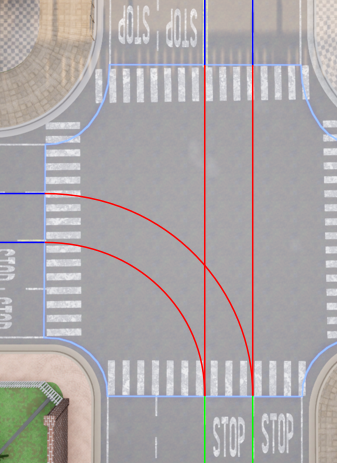
\includegraphics[width=\linewidth]{figures/chapter4/lanes-south.png}}%
    \subcaption{Incoming, connecting, and outgoing lanes (green, red, blue).}
  \end{minipage}%
  \hfill
  \begin{minipage}[t]{.3\linewidth}
    {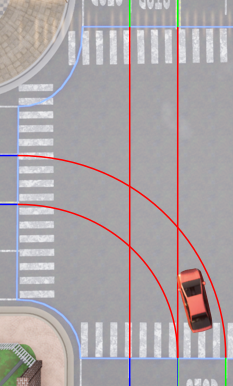
\includegraphics[width=\linewidth]{figures/chapter4/lanes-enter.png}}%
    \subcaption{A car entering a lane that intersects its route (left turn).}
  \end{minipage}%
  \hfill
  \begin{minipage}[t]{.3\linewidth}
    {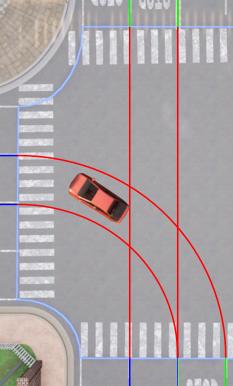
\includegraphics[width=\linewidth]{figures/chapter4/lanes-exit.png}}%
    \subcaption{A car exiting a lane that intersects its route (left turn).}
  \end{minipage}%  
  \caption{Lane events.}
  \label{fig:lane-events}%
\end{figure}% <<<


We use Python objects to represent a scenario, and reuse the data structures in Scenic's driving domain.\footnote{\url{https://scenic-lang.readthedocs.io/en/latest/libraries.html##driving-domain}}
%
The traffic rules are modeled as first-order logic sentences over the elements, attributes, states, actions, events, etc. in a scenario.
%
These sentences are represented in a logic program, more specifically an Answer Set Program.
%
In this section we explain some of the details.


%---scenery
The scenery is modeled as a road network in Scenic's driving domain.
%
A road \emph{network} is a collection of \emph{roads} and \emph{intersections}.
%
An \emph{intersection} connects two or more \emph{roads} together.
%
Each \emph{road} is a collection of \emph{lanes} and posted \emph{signs}.
%
A \emph{lane} is a polygonal region of the road together with an associated driving direction.
%
A lane is either a part of a road or a part of an intersection.
%
The \emph{incoming} lanes of an intersection are the road lanes that end at that intersection.
%
The \emph{outgoing} lanes of an intersection are the road lanes that start at that intersection.
%
The \emph{connecting} lanes of an intersection are intersection lanes that connect an incoming lane to an outgoing lane.
%
A \emph{route} is a triple of (incoming, connecting, outgoing) lanes at an intersection.
%
See Figure~\ref{fig:lane-events} for (a) two routes from the same incoming lane, and (b) two routes from different incoming lanes.
%
The connecting lanes are polygonal regions even though their boundaries appear smooth.


%---dynamic elements
A car has attributes such as shape, wheelbase, maximum steering angle, etc.
%
Scenic models the \emph{shape} of a car as a rectangle, which simplifies computing the lane events (entrance and exit).
%
The \emph{location} of a car is the location of the center of its rectangle.
%
The \emph{state} of a car in a scene specifies its \emph{pose} (location and orientation) and turn signal.
%
The \emph{behavior} of a car is the sequence of its states at each scene.
%
When the shape of a car starts overlapping a lane, it \emph{enters} the lane, and when it stops overlapping, it \emph{exits} the lane.
%
See Figure~\ref{fig:lane-events}.


%---traffic rules
The traffic rules describe right-of-way rules and abiding by traffic signs.
%
We model the traffic rules in an Answer Set Programming (ASP) language similar to~\cite{Karimi.2020}.
%
Before presenting our formulation, we need a quick introduction to ASP.
%
An ASP \emph{program} is a collection of \emph{rules} of the form:
\begin{center}
\clingo{h :- p_1, ..., p_n, not p_{n+1}, ..., not p_{n+m}.}
\end{center}
%
We call \clingo{h} the \emph{head} of the rule, and the list after \clingo{:-} is the \emph{body} of the rule.
%
The intended meaning of the above rule is
$$ p_1 \land \dots \land p_n \land  \neg p_{n+1} \land \dots \land \neg p_{n+m} \rightarrow h $$
%
Here each \emph{condition} $p_i$, as well as $h$, is an \emph{atomic predicate} over constants and variables.
%
An atomic predicate or a rule is \emph{ground} if it has no variables.
%
A \emph{fact} is a ground rule with no conditions.
%
A rule is used to infer more facts, except if the head is empty.
%
If the head is empty, we get a \emph{constraint} which means that the conjunction of predicates $p_1 \ldots \neg p_{n+m}$ should not hold true.
%
A \emph{choice rule}, which is a syntactic sugar, is a rule where the head is a list of predicates to choose from.
%
In particular,
\begin{center}
\clingo{{ h_1, ..., h_k } = N :- p_1, ..., not p_{n+m}.}
\end{center}
specifies that exactly \clingo{N} predicates from the list \clingo{h_1, ..., h_k} must be inferred if the body of the rule is true.
%
The domains of variables are determined using Herbrand semantics \cite{Herbrand.2019}, that is from all the constants mentioned in the program.
%
Given an ASP program, the ASP solver finds a set of facts (i.e. an \emph{answer set}) that is closed under the rules of the program.
%
If no such set exists, the ASP solver returns that the program is \emph{unsatisfiable}.



%---examples
Relations, actions, events, etc. in a scenario are included in an ASP program as facts.
%
For example, if the incoming lane \clingo{road8_lane0} has a stop sign, we represent this with a fact  \clingo{hasStopSign(road8_lane0)}.
%
The event of \clingo{car1} arriving at the intersection at time \clingo{t1} from the incoming lane \clingo{road8_lane0} is represented by the fact 
\begin{center}
\clingo{arrivedAtForkAtTime(car1, road8_lane0, t1)}.    
\end{center}
%
Here, \emph{fork} is an incoming lane together with its connecting lanes.
%
Traffic rules are added to a program to infer the violations.
%
For example, to infer the violations of the traffic rule \emph{``the driver of any vehicle approaching a stop sign at the entrance to an intersection shall stop''} we add
\begin{minted}[fontsize=\small]{prolog}
violatedRule(V, stopAtSign) :-
  arrivedFromIncomingLane(V, L), hasStopSign(L),
  not stoppedAtIncomingLane(V, L).
\end{minted}
%
Here, \clingo{violatedRule(V, stopAtSign)} is an atomic predicate that can be inferred to be true or false based on the grounding of variables \clingo{V} and \clingo{L}, and the truth of the rule's conditions.
%
Traffic rule violations are found simply by checking whether the answer set includes a corresponding fact.
%
In our formalization, we have two types of violations: \clingo{violatedRule(V, r)} and \clingo{violatedRightOfForRule(V1, V2, r)}.
%
The first violation involves one vehicle \clingo{V} violating a rule named \clingo{r}, and the second is a violation where vehicle \clingo{V1} violated the right-of-way of vehicle \clingo{V2} according to the traffic rule named \clingo{r}.
%
For example, the rule above is named with the term \clingo{stopAtSign}.
%
Note that upper-case terms are variables and lower-case terms are constants.
%
In the next section, we will see examples of choice rules used to search through possible orders between events, and constraints used to restrict the search space.


%---perceptible temporal order
We use the notion of \emph{perceptible order} to model ordering of events in traffic rules.
%
The parameter \emph{minimum perceptible time difference} is a threshold beyond which events are considered simultaneous from the perspective of traffic rules.
%
Suppose that $m$ represents this parameter, and let $s, t$ be two moments in time.
%
Then $s, t$ are \emph{perceptibly simultaneous} if $|s-t| < m$.
%
Otherwise, $s$ \emph{perceptibly precedes} $t$ or vice versa, if $m \leq t-s$ or $m \leq s-t$, respectively.
%
Perceptible simultaneity is not transitive since $|r-s|<m$ and $|s-t|<m$ do not imply $|r-t|<m$.
%
Therefore, perceptible order is not a partial order.
%
In contrast, \emph{temporal order}, i.e. the standard real number order of time points, is a partial order.
%
Consequently, we use separate binary relations to represent perceptible order and temporal order.



\section{Test-case Synthesis}
Given a solvable test-case (referred to as the \emph{old} test-case), the problem is to find a \emph{new} solvable test-case that is more complex.
%
We model this search problem as a constraint-satisfaction problem (CSP).
%
First we explain this search problem, then we present our search algorithm.

\subsection{Test-case search problem}
\label{sec:problem}

\begin{figure}
\centering
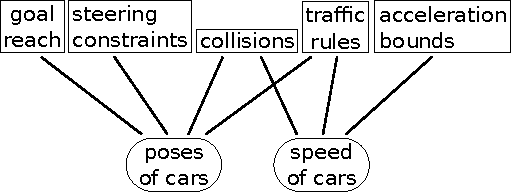
\includegraphics[width=70mm]{figures/chapter4/problem.pdf}%
\caption{Test-case CSP problem.}
\label{fig:problem}%
\end{figure}

%---search variables and parameters
The \emph{search variables} are the behaviors of the new non-egos, a \emph{complexity certificate}, and a \emph{solvability certificate}.
%
The \emph{complexity certificate} is an ego behavior that solves the old test-case, but fails the new test-case.
%
The \emph{solvability certificate} is an ego behavior that solves the new test-case.
%
The set of new non-egos and their routes through the intersection are given as parameters rather than as search variables.%
\footnote{The reason we did not extend our algorithm to automatically select values for these parameters is that it is not clear how to do significantly better than a brute-force approach.
%
Furthermore, a manual parameter assignment gives more control over the search.}
%
As discussed in the previous section, we do not change the behaviors of the old non-egos so they are fixed parameters.
%
The rest of the parameters, such as the scenery and traffic rules, are given by the old test-case.


%---constraints
There are three types of constraints imposed by the pass-fail criteria, to generate a more-complex and solvable test-case.
%
First is collision avoidance, which regards the shape of each car, and its location and orientation at each time relative to other cars.
%
The locations and orientations are themselves constrained by physics, such as limited forces available to accelerate or brake, and bounded range for steering angles.
%
Second is goal-reach, which regards overlap of a trajectory with a region in the scenery.
%
This in turn is constrained by physics of car motion, and also the scenery.
%
Third is traffic rules, which regards the lane events, stop events, etc.
%
This depends on the logic of traffic rules, geometry of lanes, location and orientation of the cars at each time, also each car's shape.
%
The space of possible complexity and solvability certificates depends on the choice of new non-ego behaviors.
%
Therefore, the search for the new non-egos has to be done simultaneously as the search for the certificates.


%---proposed strategy
Our proposed approach is to decompose the CSP problem into three subproblems, where each subproblem is suitable to a specialized technique.
%
In particular, we use simulation and closed-loop control to find a sequence of poses that satisfies the steering constraints and goal-reach.
%
We use ASP to find possible orderings of events that satisfy the required traffic rules violations or compliance.
%
Finally, we use SMT to find timing of poses that satisfy the analytical constraints on the longitudinal motion e.g. smoothness of speed, bounded longitudinal acceleration, negligible speed at stop events, etc.
%
Our decomposition of the problem is shown in Figure~\ref{fig:problem}.
%
The first subproblem finds the poses of cars, while the second and third subproblems find the speed of cars.


%---constraints on new non-egos
The new non-egos should not collide with the old non-egos since a collision may alter an old non-ego's trajectory which violates our guarantee of comparability of test-case complexities.


%---constraints on complexity certificate
The complexity certificate is an ego behavior that passes the old test-case, but fails the new test-case.
%
The constraints that guarantee such a behavior are as follows.
%
The behavior should avoid colliding with the old non-egos, respect traffic signs and the right-of-way of old non-egos, and reach ego's goal, to pass the old test-case.
%
The behavior should avoid colliding with the new non-egos, so that it is a physically valid behavior in the old test-case where the collision forces of the new non-egos are absent.
%
Since the behavior respects traffic signs and does not collide with the new non-egos, the only way for it to fail the new test-case is to violate the right-of-way of at least one of the new non-egos.


%---solvability certificate
The solvability certificate is an ego behavior that passes the new test-case.
%
That is, the behavior does not collide with the old or new non-egos, respects traffic signs and the right-of-way of both the old and new non-egos, and reaches ego's goal.







\subsection{Test-case generation algorithm}

\begin{figure}
\centering
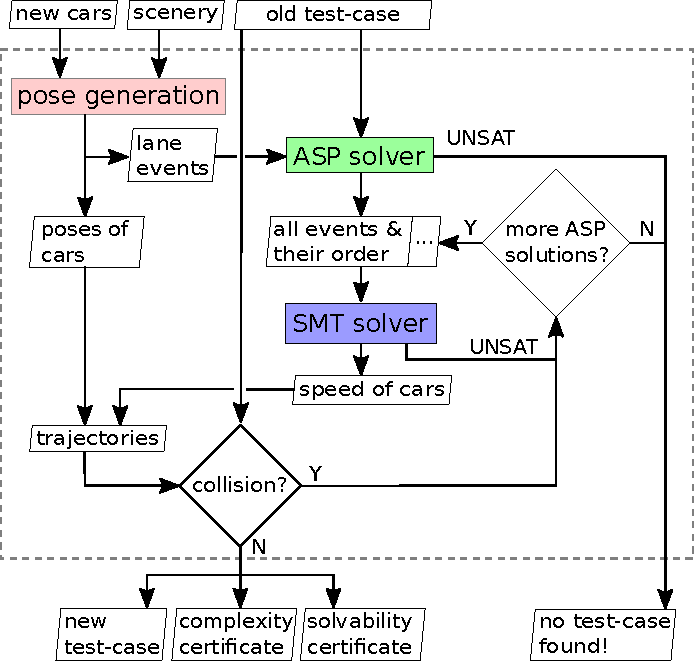
\includegraphics[width=85mm]{figures/chapter4/algorithm.pdf}%
\caption{The test-case generation algorithm.}
\label{fig:algorithm}%
\end{figure}

Our algorithm has three main steps.
%
These steps are highlighted with red, green and blue in Figure~\ref{fig:algorithm}.

%---------------------
\subsubsection{Step 1: pose generation}
The first step is to determine the poses of each car such that they satisfy the car's \emph{steering constraints}.
%
Two consecutive poses $p_1, p_2$ at times $t_1, t_2$ respectively, satisfy the constraint if and only if there exists a steering input as a function of time over the interval $[t_1, t_2]$ that drives the car from $p_1$ to $p_2$.
%
Note that a pose specifies both the location and the orientation of the car.
%
The constraint depends on the steering mechanism of each car e.g. steering axles, maximum steering angles, wheelbase, etc.

%---simulation
The algorithm drives each car using a steering controller in a physics simulation, so the generated pose-sequence satisfies the steering constraints.
%
The steering controller tracks the centerline of the car's route.
%
A speed controller is used to track a constant speed.
%
See Figure~\ref{fig:sim-pose} for a pose sequence.
%
A location is shown by a dot and the orientation is implied by the tangent to the dot sequence.

%---success
If the two ego trajectories (candidates for complexity and solvability certificates) reach ego's goal, our algorithm proceeds to Step 2.
%
Note that the new non-egos do not need to reach their goal.

%---failure
Otherwise, the algorithm stops and returns with failure.
%
If we have a solvability certificate for the old test-case, we can simply use its poses and skip the simulations of ego, so Step 1 would not fail.

\begin{figure}
\centering
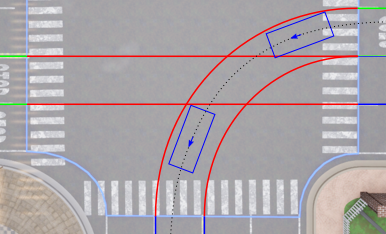
\includegraphics[width=60mm]{figures/chapter4/sim-poses-landscape.png}%
\caption{Two poses at which lane events happen are shown with arrows, and the car's shape with rectangles.}
\label{fig:sim-pose}%
\end{figure}


%-----------second step----------
\subsubsection{Step 2: deciding order of events}
This step finds all possible order of events such that one of the ego behaviors would qualify as a complexity certificate, and the other as a solvability certificate.
%
The set of events and their perceptible order affect the traffic rules violations.
%
Some of this information is already fixed by the behavior of old non-egos.
%
The lane events of each new car are computed from its pose sequence from Step 1, the car's shape, and scenery's lane geometry.
%
Furthermore, for each car, the temporal order between its lane events are implied by the poses at which they happen and the order between poses in the sequence.
%
Each event is assigned a symbolic time such that simultaneous lane events are assigned the same time symbol.
%
It remains to determine what stop events should happen and what is the perceptible order between all events.

%---CSP
Therefore, this step is a CSP where the \emph{search variables} are the stop events and the perceptible order between events.
%
The search space is finite since there are only a finite number of events and possible order between them.
%
The \emph{constraints} include the old events and their temporal and perceptible order, the new lane events and their temporal order, and
the complexity and solvability criteria.
%
Our algorithm specifies this search problem as an ASP program and solves it with an ASP solver.



%---perceptible order 
The perceptible order between time symbols is represented by two binary relations  \clingo{equal()} and \clingo{lessThan()}.
%
If we instruct the ASP solver to make a choice about the perceptible order of every pair of time symbols, we make the search space unnecessarily big.
%
Instead, we manually go through the set of traffic rules and add a choice rule only for each pair of events that their perceptible order matters to the right-of-way violations.
%
This manual derivation has to be done only once for each traffic rule, say after modeling the traffic rules for an intersection.
%
For example, consider the traffic rule 
\begin{quote}
``The driver of a vehicle approaching an intersection shall yield the right-of-way
to any vehicle which has entered the intersection from a different highway,''    
\end{quote}
and its ASP encoding
\begin{minted}[fontsize=\small]{prolog}
violatesRightOfForRule(V1, V2, yieldToInside):-
  enteredForkAtTime(V1, F1, Te1),
  enteredForkAtTime(V2, F2, Te2),
  onDifferentHighways(F1, F2),
  requestedLane(V1, L1), requestedLane(V2, L2),
  overlaps(L1, L2),
  lessThan(Te2, Te1),
  leftLaneAtTime(V2, L1, T1),
  enteredLaneAtTime(V1, L2, T2),
  lessThan(T2, T1).
\end{minted}
%
For this rule, we only need a choice for \clingo{lessThan(Te2, Te1)}:
\begin{minted}[fontsize=\small]{prolog}
{equal(Te1,Te2); lessThan(Te1,Te2); lessThan(Te2,Te1)}=1 :- 
  enteredForkAtTime(V1, F1, Te1),
  enteredForkAtTime(V2, F2, Te2),
  onDifferentHighways(F1, F2), 
  requestedLane(V1, L1), requestedLane(V2, L2),
  overlaps(L1, L2).
\end{minted}
and a choice for \clingo{lessThan(T2, T1)}:
\begin{minted}[fontsize=\small]{prolog}
{equal(T1, T2); lessThan(T1, T2); lessThan(T2, T1) } = 1 :-
  enteredForkAtTime(V1, F1, Te1),
  enteredForkAtTime(V2, F2, Te2),
  onDifferentHighways(F1, F2),
  requestedLane(V1, L1), requestedLane(V2, L2),
  overlaps(L1, L2),
  lessThan(Te2, Te1),
  leftLaneAtTime(V2, L1, T1),
  enteredLaneAtTime(V1, L2, T2).
\end{minted}

%---temporal order
Temporal order is different from perceptible order as discussed earlier.
%
The temporal order between time symbols is represented using a binary relation \clingo{realLTE()}.
%
The `LTE' stands for Less-Than-or-Equal-to and emphasizes that the binary relation is a partial order (and so transitive).
%
The `real' emphasizes the intended meaning of this relation as the order between real numbers.
%
The order between real numbers is total but  \clingo{realLTE()} is partial, since the temporal order between lane events of two different cars are not physically constrained and may not matter to traffic rules violations either.
%
In particular, time symbols \clingo{s,t} are simultaneous if and only if
\clingo{realLTE(s,t)} and \clingo{realLTE(t,s)}, \clingo{s} precedes \clingo{t} if and only if 
\clingo{realLTE(s,t)} and \clingo{not realLTE(t,s)}, and the order is unknown (and unimportant) if and only if \clingo{not realLTE(s,t)} and \clingo{not realLTE(t,s)}.
%
For each new car, the temporal order between its lane events are already determined by Step 1, and are added as facts to the ASP program.

%---new lane events
The new lane events, determined from Step 1, are added to the ASP program as facts.
%
The time symbol of each event is used as a parameter of the fact.
%
For example, the term \clingo{t1} in the fact
\clingo{enteredLaneAtTime(car1, road258_lane0, t1)} is its time symbol.


%---old events
Each old event is also added to the ASP program as a fact.
%
Even though the real number value of time is known for old events, time symbols are instantiated so that old events can be represented as facts in the ASP program.
%
The temporal and perceptible order of old events are determined from the numerical time of those events.
%
The temporal and perceptible order between an old event and a new event is not a known fact and will be determined by the choice rules.


%---occurrence of stop and turn signal events
The occurrence of a stop event (at a stop sign) is a search variable, so we instruct the ASP solver to make a choice:
\begin{minted}[fontsize=\small]{prolog}
{stoppedAtForkAtTime(V, F, @time(V, stop))} = 1 :-
  arrivedAtFork(V, F), hasStopSign(F),
  not violatedRule(V, stopAtSign).
\end{minted}
%
The term \clingo{@time(V, stop)} is simply the time symbol assigned to the stop event of car \clingo{V}.
%
If a stop event happens, then it must be perceptibly after the car has arrived at the intersection and perceptibly before it entered the intersection.
\begin{minted}[fontsize=\small]{prolog}
lessThan(T1, T) :-  
  arrivedAtForkAtTime(V, F, T1),
  stoppedAtForkAtTime(V, F, T).
lessThan(T, T2) :-
  stoppedAtForkAtTime(V, F, T),  
  enteredForkAtTime(V, F, T2).
\end{minted}



%---complexity
The ego behavior that is a candidate for a complexity certificate must satisfy the following constraints.
%
Let \clingo{illegal} be the name of the car, \clingo{v1,...,vN} be the list of new non-egos, and \clingo{old()} be true of the old non-egos.
%
The first constraint says that \clingo{illegal} does not violate the right-of-way of old non-egos:
\begin{minted}[fontsize=\small]{prolog}
:- old(V), violatesRightOf(illegal, V).
\end{minted}
%
The second constraint says that \clingo{illegal} does not violate any other traffic rules, say stopping at a stop sign:
\begin{minted}[fontsize=\small]{prolog}
:- violatesRule(illegal, _).
\end{minted}
%
These two constraints require \clingo{illegal}'s behavior to be a solution for the old test-case.
%
The third constraint says that \clingo{illegal} violates the right-of-way of at least one of the new non-egos:
\begin{minted}[fontsize=\small]{prolog}
:- not violatesRightOf(illegal, v1), ..., 
   not violatesRightOf(illegal, vN).
\end{minted}
%
Hence \clingo{illegal}'s behavior fails the new test-case.


%---solvability certificate
The ego behavior that is a candidate for a solvability certificate must satisfy the following constraints.
%
Let \clingo{ego} be the name of the car, and \clingo{nonego()} be true of both the old and the new non-egos.
%
The first constraint says that \clingo{ego} does not violate the right-of-way of any non-egos:
\begin{minted}[fontsize=\small]{prolog}
:- nonego(V), violatedRightOf(ego, V).
\end{minted}
%
The second constraint says that \clingo{ego} does not violate any other traffic rules either:
\begin{minted}[fontsize=\small]{prolog}
:- violatedRule(ego, _).
\end{minted}
%
Hence \clingo{ego}'s behavior solves the new test-case.


%---no ASP solutions
If there are no ASP solutions, the ASP solver returns `unsatisfiable' and our algorithm stops with failure.

%---ASP solutions
If the ASP program is satisfiable, the ASP solver enumerates all the solutions, which are finitely many.
%
This step passes the ASP solutions one-by-one to the next step to check if each yields a final solution.
%
If a final solution is found (in Step 3), the algorithm either stops and returns the result, or it tries to find more solutions by continuing through the list of ASP solutions, depending on which option the user wants.



%-----------third step-----------
\subsubsection{Step 3: generating the speed of cars}
In this step we determine how fast each car moves along its sequence of poses fixed in Step 1.
%
The speed profile determines the time at which each lane event or stop event happens, which must preserve the order relations fixed in Step 2.
%
This step is again a CSP where the \emph{search variables} are numerical values of the new time symbols, and a time-to-distance-travelled mapping for each car.
%
The speed of a car is the slope of this mapping.
%
The \emph{constraints} include occurrence of stop events, the relations \clingo{realLTE()}, \clingo{lessThan()}, and \clingo{equal()} between time symbols, numerical values of old time symbols, and bounds on longitudinal accelerations.
%
Our algorithm specifies this search problem as a system of polynomial equations and inequalities and solves it with an SMT solver.

\begin{figure}
\centering
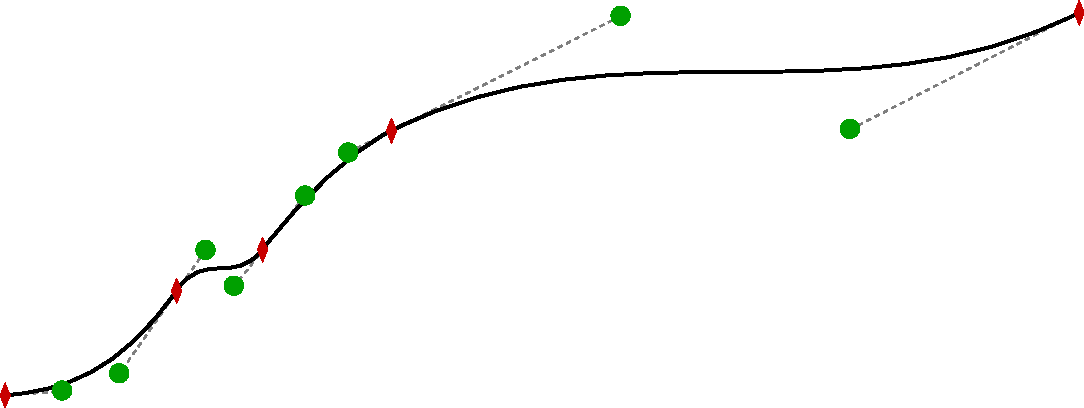
\includegraphics[width=\linewidth]{figures/chapter4/composite-bezier.pdf}
\caption{A composite cubic Bezier curve.}
\label{fig:composite-Bezier}
\end{figure}


%---search variables: time of time symbols
A real-valued variable $T$ is assigned for each new time symbol $t$ that appears in \clingo{equal()}, \clingo{lessThan()}, or a stop event.
%
These are the only new time symbols that are potentially consequential to traffic rules, due to our custom choice rules (in Step 2) for perceptible order.%
\footnote{This restriction reduces the number of search variables and constraints, thus simplifies the SMT search problem significantly.}
%
The rest of the new time symbols are for lane events (that were not consequential to the right-of-way violations,) and their numerical value can be determined from their car's time-to-distance-travelled mapping (after it is found) and their distance.


%---composite Bezier curves introduction
We use piecewise cubic polynomial functions in the form of composite Bezier curves to represent the distance travelled by a car as function of time.
%
The coefficients of the polynomials are in the form of \emph{control points}.
%
The crucial property for our purposes is the \emph{local control property}.
%
That is, changing a control point, affects the function only locally.
%
For example, if an SMT solver has fixed the first few control points to control the speed of a car before entering the intersection, it can change later control points, say for inside the intersection, without invalidating the speed before entrance.
%
\emph{Cubic} Bezier curves have four control points.
%
The first and the last control points are \emph{interpolating} points, meaning that the curve passes through those points.
%
The second and the third points determine the slope of the curve at the first and the last point, respectively.
%
See Figure~\ref{fig:bezier} for examples.
%
A \emph{composite} Bezier curve is a sequence of Bezier curves where the end of each segment is the start of the next segment.
%
See Figure~\ref{fig:composite-Bezier} for an example.
%
The red diamonds and green dots indicate the interpolating and intermediate control points of the segments, respectively.
%
See \cite{Farin.2002} for more on Bezier curves.


%---search variables: time-to-distance mapping
The representation of a time-to-distance mapping is as follows.
%
For each pair of time variables $T_i, T_{i+1}$ of a car that are consecutive (with respect to the \clingo{realLTE()} order between their time symbols), a cubic Bezier segment is instantiated.
%
The four control points of the segment are $(T_i, d_i)$, $(T_i + \frac{T_{i+1}-T_i}{3}, d_{i,1})$, $(T_i + \frac{2(T_{i+1}-T_i)}{3}, d_{i,2})$, and $(T_{i+1}, d_{i+1})$.
%
Here $d_{i,1}$ and $d_{i,2}$ are real-valued variables;
$d_i$ is the travelled distance for the event corresponding to $T_i$ which is a determined number for a lane event, and a real-valued variable otherwise; and $d_{i+1}$ is defined similarly.
%
Furthermore, the first segment has the control points $(0, 0)$, $(\frac{T_1}{3}, d_{0,1})$, $(\frac{2T_1}{3}, d_{0,2})$, $(T_1, d_1)$; and the last segment has the control points $(T_n, d_n)$, $(T_n + \frac{T_M-T_n}{3}, d_{n,1})$, $(T_n + \frac{2(T_M-T_n)}{3}, d_{n,2})$, $(T_M, d_M)$, where is $T_M$ is the duration of the scenario, and $d_M$ is the total travelled distance of the car as determined in Step 1.


%---temporal constraints
The perceptible order constraint is specified as follows.
%
For a time symbol $t$, let $v(t)$ be its numerical value if $t$ is for an old event, otherwise let $v(t)$ be its assigned time variable $T$.
%
Now for any time variable $S$, if \clingo{equal(s,t)} or \clingo{equal(t,s)} then we require $|S-v(t)| < m$, if \clingo{lessThan(s,t)} then we require $m \leq v(t)-S$, and if \clingo{lessThan(t,s)} then we require $m \leq S-v(t)$, where $m$ is the minimum perceptible time difference.
%
As for temporal order, if \clingo{realLTE(s,t)} and \clingo{not realLTE(t,s)} then we require $S < v(t)$.
%
Similarly if \clingo{realLTE(t,s)} and \clingo{not realLTE(s,t)} then we require $v(t) < S$.

%---no new lane events
\begin{figure}% >>>
  \centering
  \begin{minipage}[t]{.495\linewidth}
    {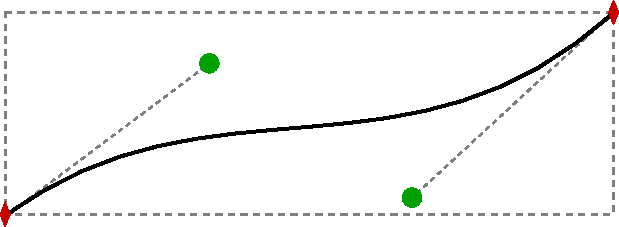
\includegraphics[width=\linewidth]{figures/chapter4/bezier-monotonic.pdf}}%
    \subcaption{Curve bounded between the heights of endpoints.}
  \end{minipage}%
  \hfill
  \begin{minipage}[t]{.495\linewidth}
    {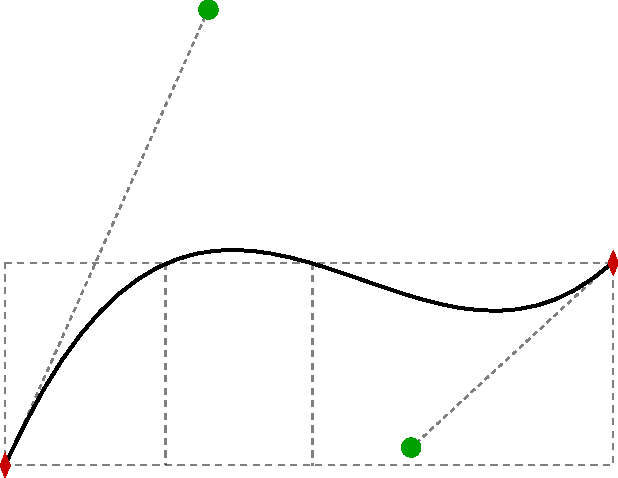
\includegraphics[width=\linewidth]{figures/chapter4/bezier-nonmonotonic.pdf}}%
    \subcaption{Curve created a new lane event at a vertical dotted line.}
  \end{minipage}%
  \caption{No-new-lane-event constraint.}\label{fig:bezier}%
\end{figure}% <<<

%---no new lane events
We must ensure that the Bezier interpolation does not create new lane events consequential to right-of-way.
%
In Figure~\ref{fig:bezier}(b), suppose that the right endpoint of the curve represents entering a lane.
%
The height of the curve reaches the height of the right endpoint at the vertical dotted lines which implies that the car enters the lane sooner than intended.
%
We prevent new lane events by requiring that the heights of the intermediate control points be between the heights of the endpoints.
%
$$ d_i \leq d_{i,1} \leq d_{i+1}, \quad d_i \leq d_{i,2} \leq d_{i+1}.
$$
%
Then the convex hull property implies that the whole interpolated Bezier segment stays within its endpoint heights, e.g. as in Figure~\ref{fig:bezier}(a).





%---longitudinal acceleration bounds
The longitudinal acceleration constraints are as follows.
%
The second derivative of a cubic polynomial is linear so its extrema over a closed interval are achieved at the endpoints.
%
For an interval $[T_i, T_{i+1}]$, the second derivatives at endpoints are
$$
a_i = \frac{6(d_i-2d_{i,1}+d_{i,2})}{(T_{i+1}-T_i)^2}, \quad
a_{i+1} = \frac{6(d_{i,1}-2d_{i,2}+d_{i+1})}{(T_{i+1}-T_i)^2}.
$$
%
Therefore, if $a_m$ and $a_M$ are respectively the minimum and maximum bounds on longitudinal acceleration, we require
$$ a_m \leq a_i \leq a_M, \quad a_m \leq a_{i+1} \leq a_M.
$$
%
These inequalities are quadratic since we can remove the fractions by multiplying the inequalities by $(T_{i+1}-T_i)^2$.


%---smooth speed
Our scenarios do not include collision events, as discussed in \S\ref{sec:problem}, so the speed of a car, i.e. the slope of the time-distance curve, must be continuous.
%
Each segment of a composite Bezier curve is a smooth function since it is a polynomial.
%
At interpolating points between two consecutive segments, we force the slopes on both sides to be equal with the quadratic equation
$$ \frac{d_i-d_{i-1,2}}{T_i-T_{i-1}} = \frac{d_{i,1}-d_i}{T_{i+1}-T_i}.
$$

%---stop events constraints
A stop event implies a constraint on the instantaneous speed of the car.
%
If $T_i$ is a time variable for a stop event, we require the instantaneous speed at $T_i$ to be within a threshold $v_{stop} \geq 0$:
$$ \frac{d_{i,1}-d_i}{\frac{1}{3}(T_{i+1}-T_i)} \leq v_{stop} $$
%
If a car violates a stop sign, we require the instantaneous speed between arrival at and entrance to the intersection to be at least a threshold $v_{run}$ where $v_{run} > v_{stop}$.
%
It is sufficient to force the slope to not have a local minimum over the interval, and the slopes at the endpoints to be at least $v_{run}$.
%
For the slope of the function to not have a local minimum over the interval, the second derivative should not change from negative to positive:
$$
\lnot (a_i < 0 \;\land\; a_{i+1} > 0)
$$
which is equivalent to the linear inequalities
$$ d_i-2d_{i,1}+d_{i,2} \geq 0 \;\lor\; d_{i,1}-2d_{i,2}+d_{i+1} \leq 0.
$$
%
The lower bound on endpoint slopes are specified with the linear inequalities
$$ \frac{d_{i,1}-d_i}{\frac{1}{3}(T_{i+1}-T_i)} \geq v_{run}, \quad \frac{d_{i+1}-d_{i,2}}{\frac{1}{3}(T_{i+1}-T_i)} \geq v_{run}.
$$

%---no SMT solution
If the SMT solver returns `unsatisfiable', Step 3 is repeated with the next ASP solution, if any.
%
If no ASP solution remains, the algorithm returns with no solutions.

%---SMT solution
If the SMT solver returns a solution, i.e. coordinates of the control points, we can sample points on the time-distance curves using the standard de Casteljau algorithm for Bezier curve computation.
%
This gives the time-to-distance-travelled mapping.
%
Composing this with the travelled distance at each pose, we get the pose at each time.

\section{Evaluation}
\label{sec:evalsetup}

We demonstrate the capabilities of our approach by generating test-cases for three different situations:
\begin{enumerate}
\item left turn at a multi-lane 4-way stop,
\item left turn at a T-intersection from the continuing highway to the terminating highway,
\item left turn at a 3-way uncontrolled Y-intersection.
\end{enumerate}
%
For each of these static environments, we generate a sequence of increasingly complex test-cases.
%
The videos and logs of the test-cases, also the traffic rules' encoding in Clingo \cite{Gebser.2018}, are available on the web\footnote{\url{https://www.dropbox.com/sh/e6q4hw98ert5yj7/AAAgo7IlYRKg-rYs7Q9GyMx9a?dl=0}}.
%
The solvability and complexity certificates are visualized in the videos with green and red egos, respectively.


%---executing test-cases
CARLA has several built-in autopilot software that have access to the full simulation state.
%
We subject two specific autopilot agents to the test suite which are automatically generated by our algorithm.
%
We observe that autopilot can fail as we increase the complexity of the test-cases.
%
Finally, we test CARLA's autopilot when  Intel's Responsibility Sensitive Safety (RSS) is added to safeguard autopilot's actions.
%
We observe fewer failures when RSS is enabled, but still autopilot-plus-RSS doesn't pass all the test-cases.


%---the challenge of solving the problem
Our straightforward attempt using Scenic's probabilistic programming failed to find solutions to the search problem.
%
The search space is uncountably infinite so there are too many ways to modify a failed sample.
%
On the other hand, the solution space is highly restricted with continuous and discrete constraints and intertwined dependencies, as explained in the previous section.
%
More specifically, traffic rules depend on only a few discrete events, so they partition the search space into big equivalence classes.
%
Probabilistic mutation of trajectories is searching for a target class by walking within big classes and looking for their boundaries.
%
In contrast, our ASP approach is identifying all the target classes by looking from the above, then searching for a sample within each of them.

\subsection{Results}
We use Scenic \cite{Fremont.2020} as an interface to CARLA to execute a generated test-case, e.g. to test CARLA's autopilot (playing the role of ego).


%---------------------------------------
\begin{figure}[ht]% >>>
  \centering
  \begin{minipage}[t]{.499\linewidth}
    {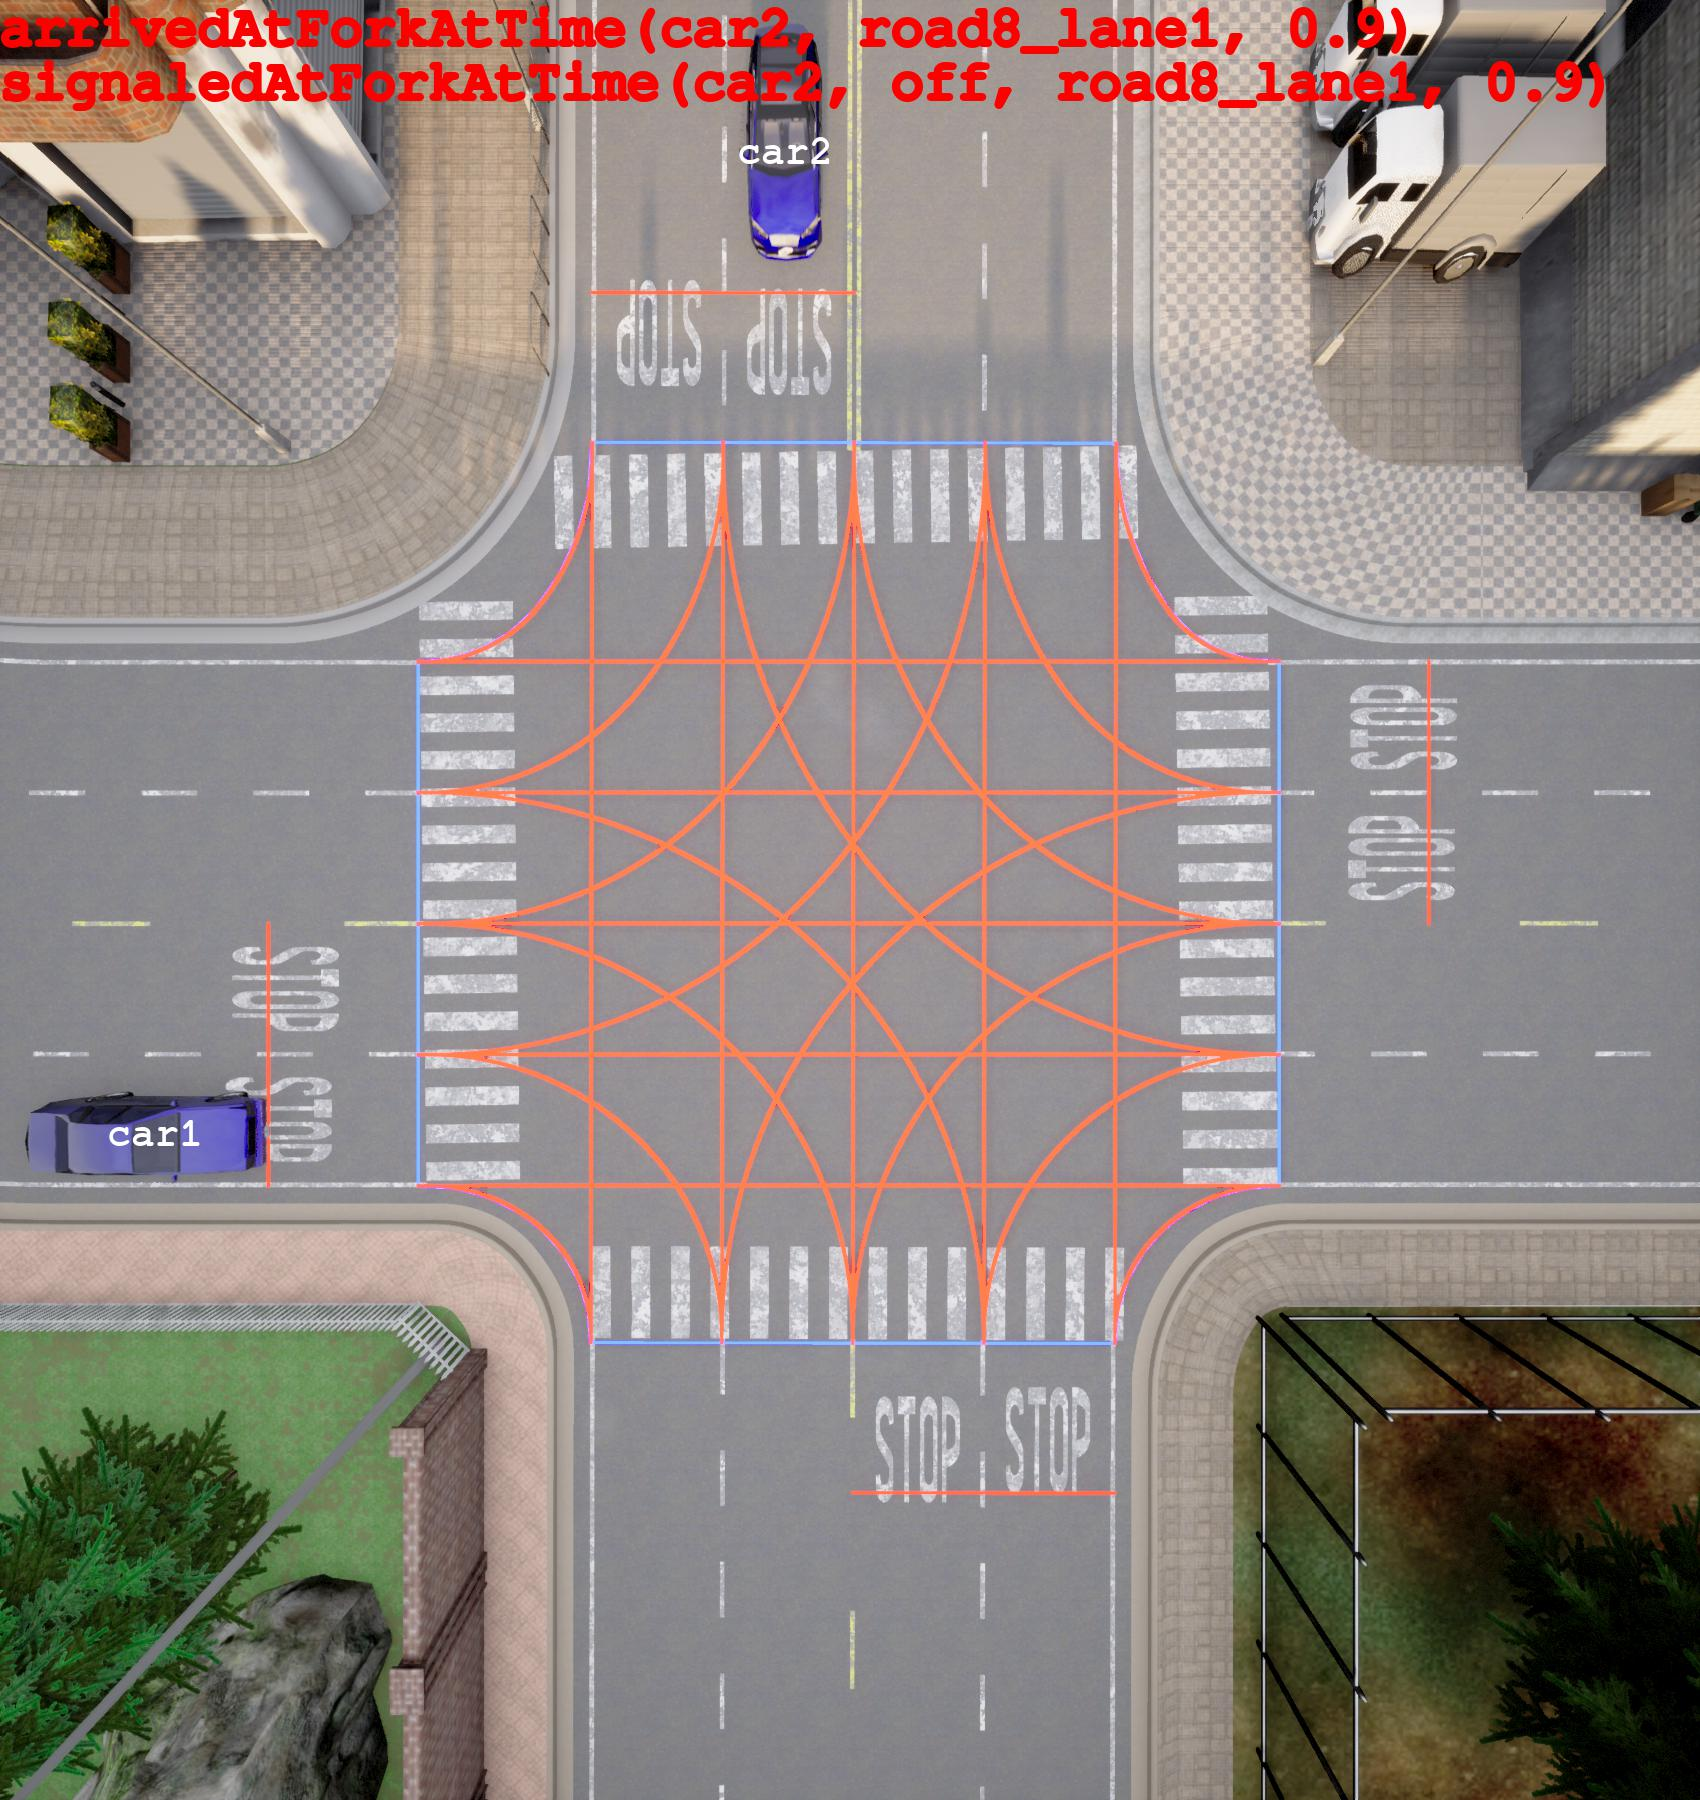
\includegraphics[width=\linewidth]{figures/chapter4/2_18.jpg}}%
    \subcaption{car2 arrives.}
  \end{minipage}%
  \hfill
  \begin{minipage}[t]{.499\linewidth}
    {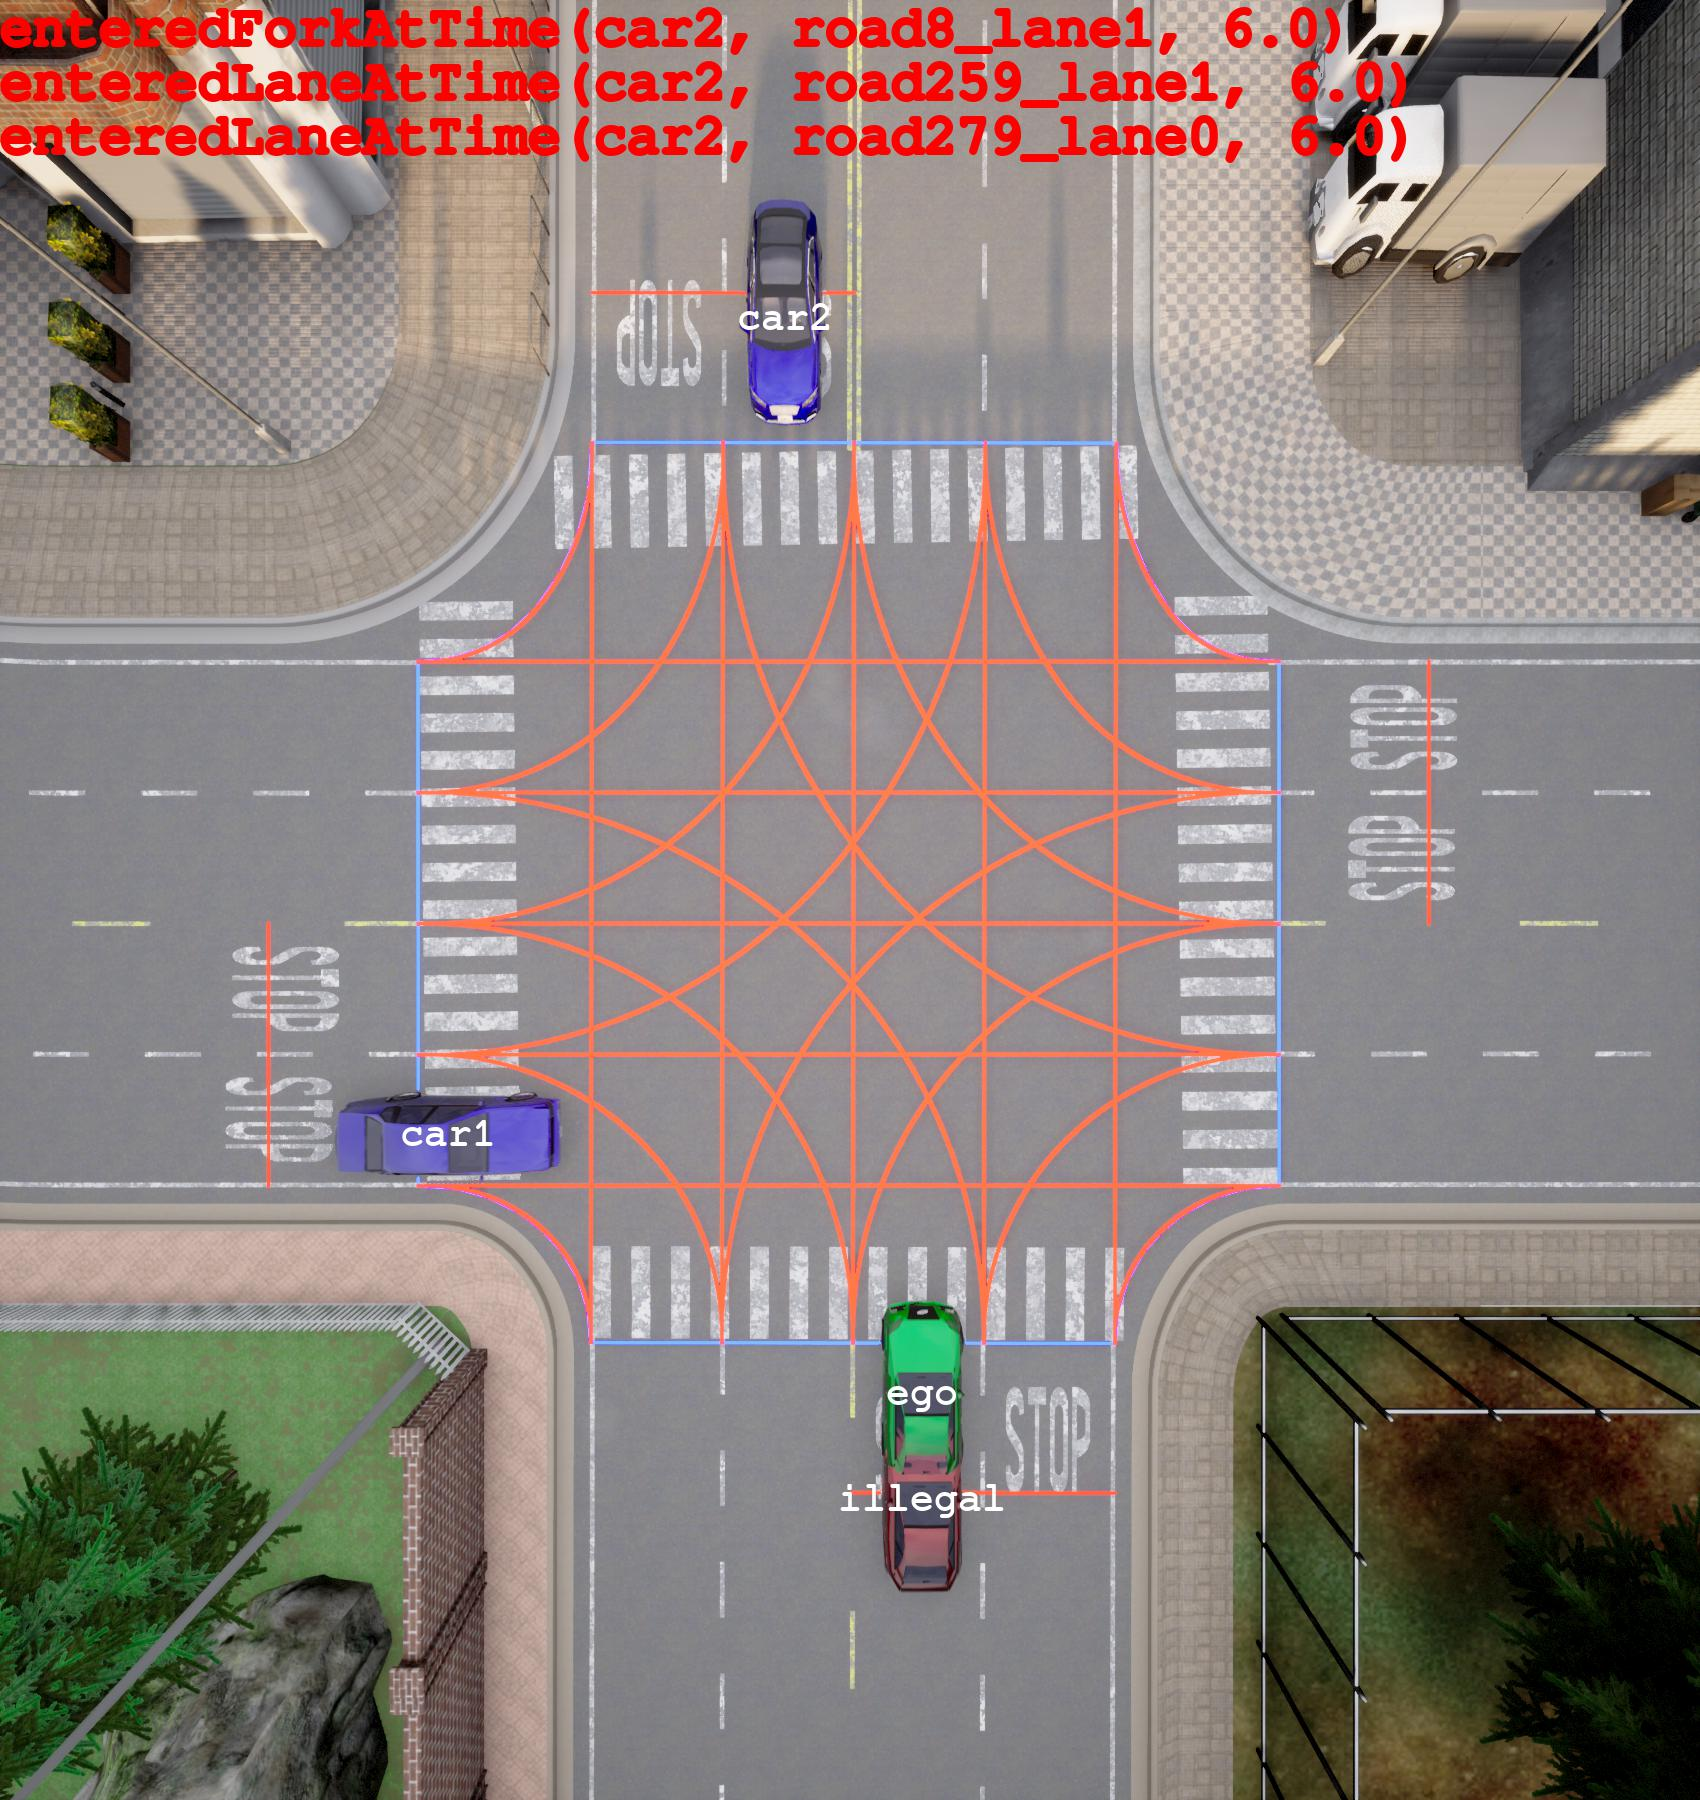
\includegraphics[width=\linewidth]{figures/chapter4/2_120.jpg}}%
    \subcaption{car2 enters.}
  \end{minipage}%
  \hfill
  \begin{minipage}[t]{.499\linewidth}
    {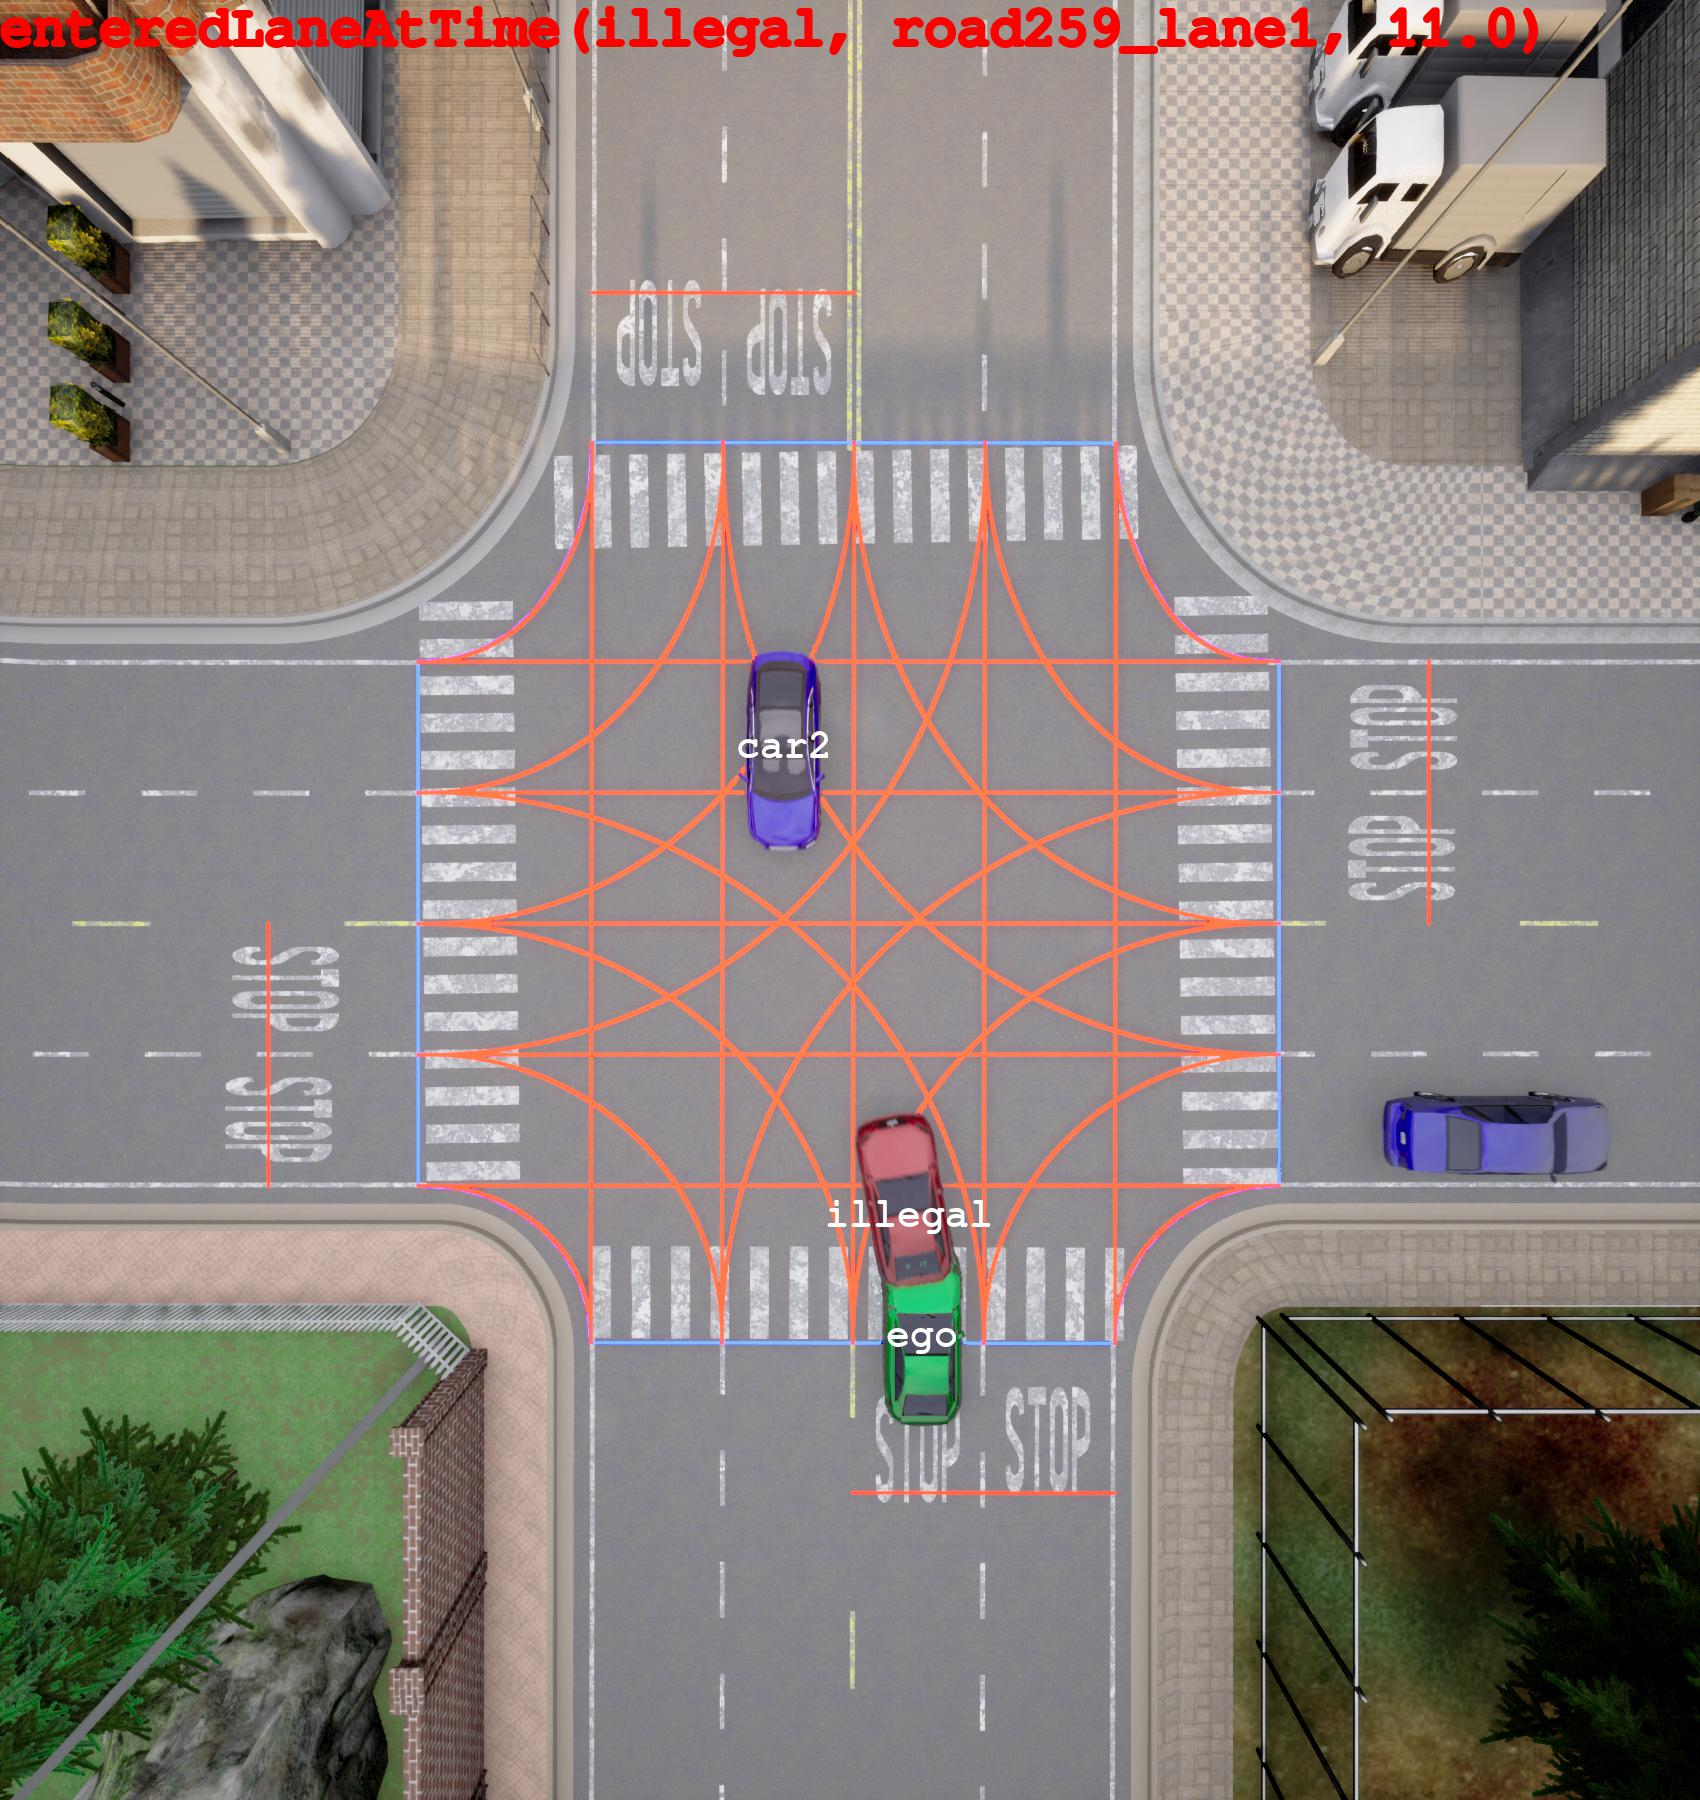
\includegraphics[width=\linewidth]{figures/chapter4/2_220.jpg}}%
    \subcaption{illegal enters car2's route.}
  \end{minipage}%
  \hfill
  \begin{minipage}[t]{.499\linewidth}
    {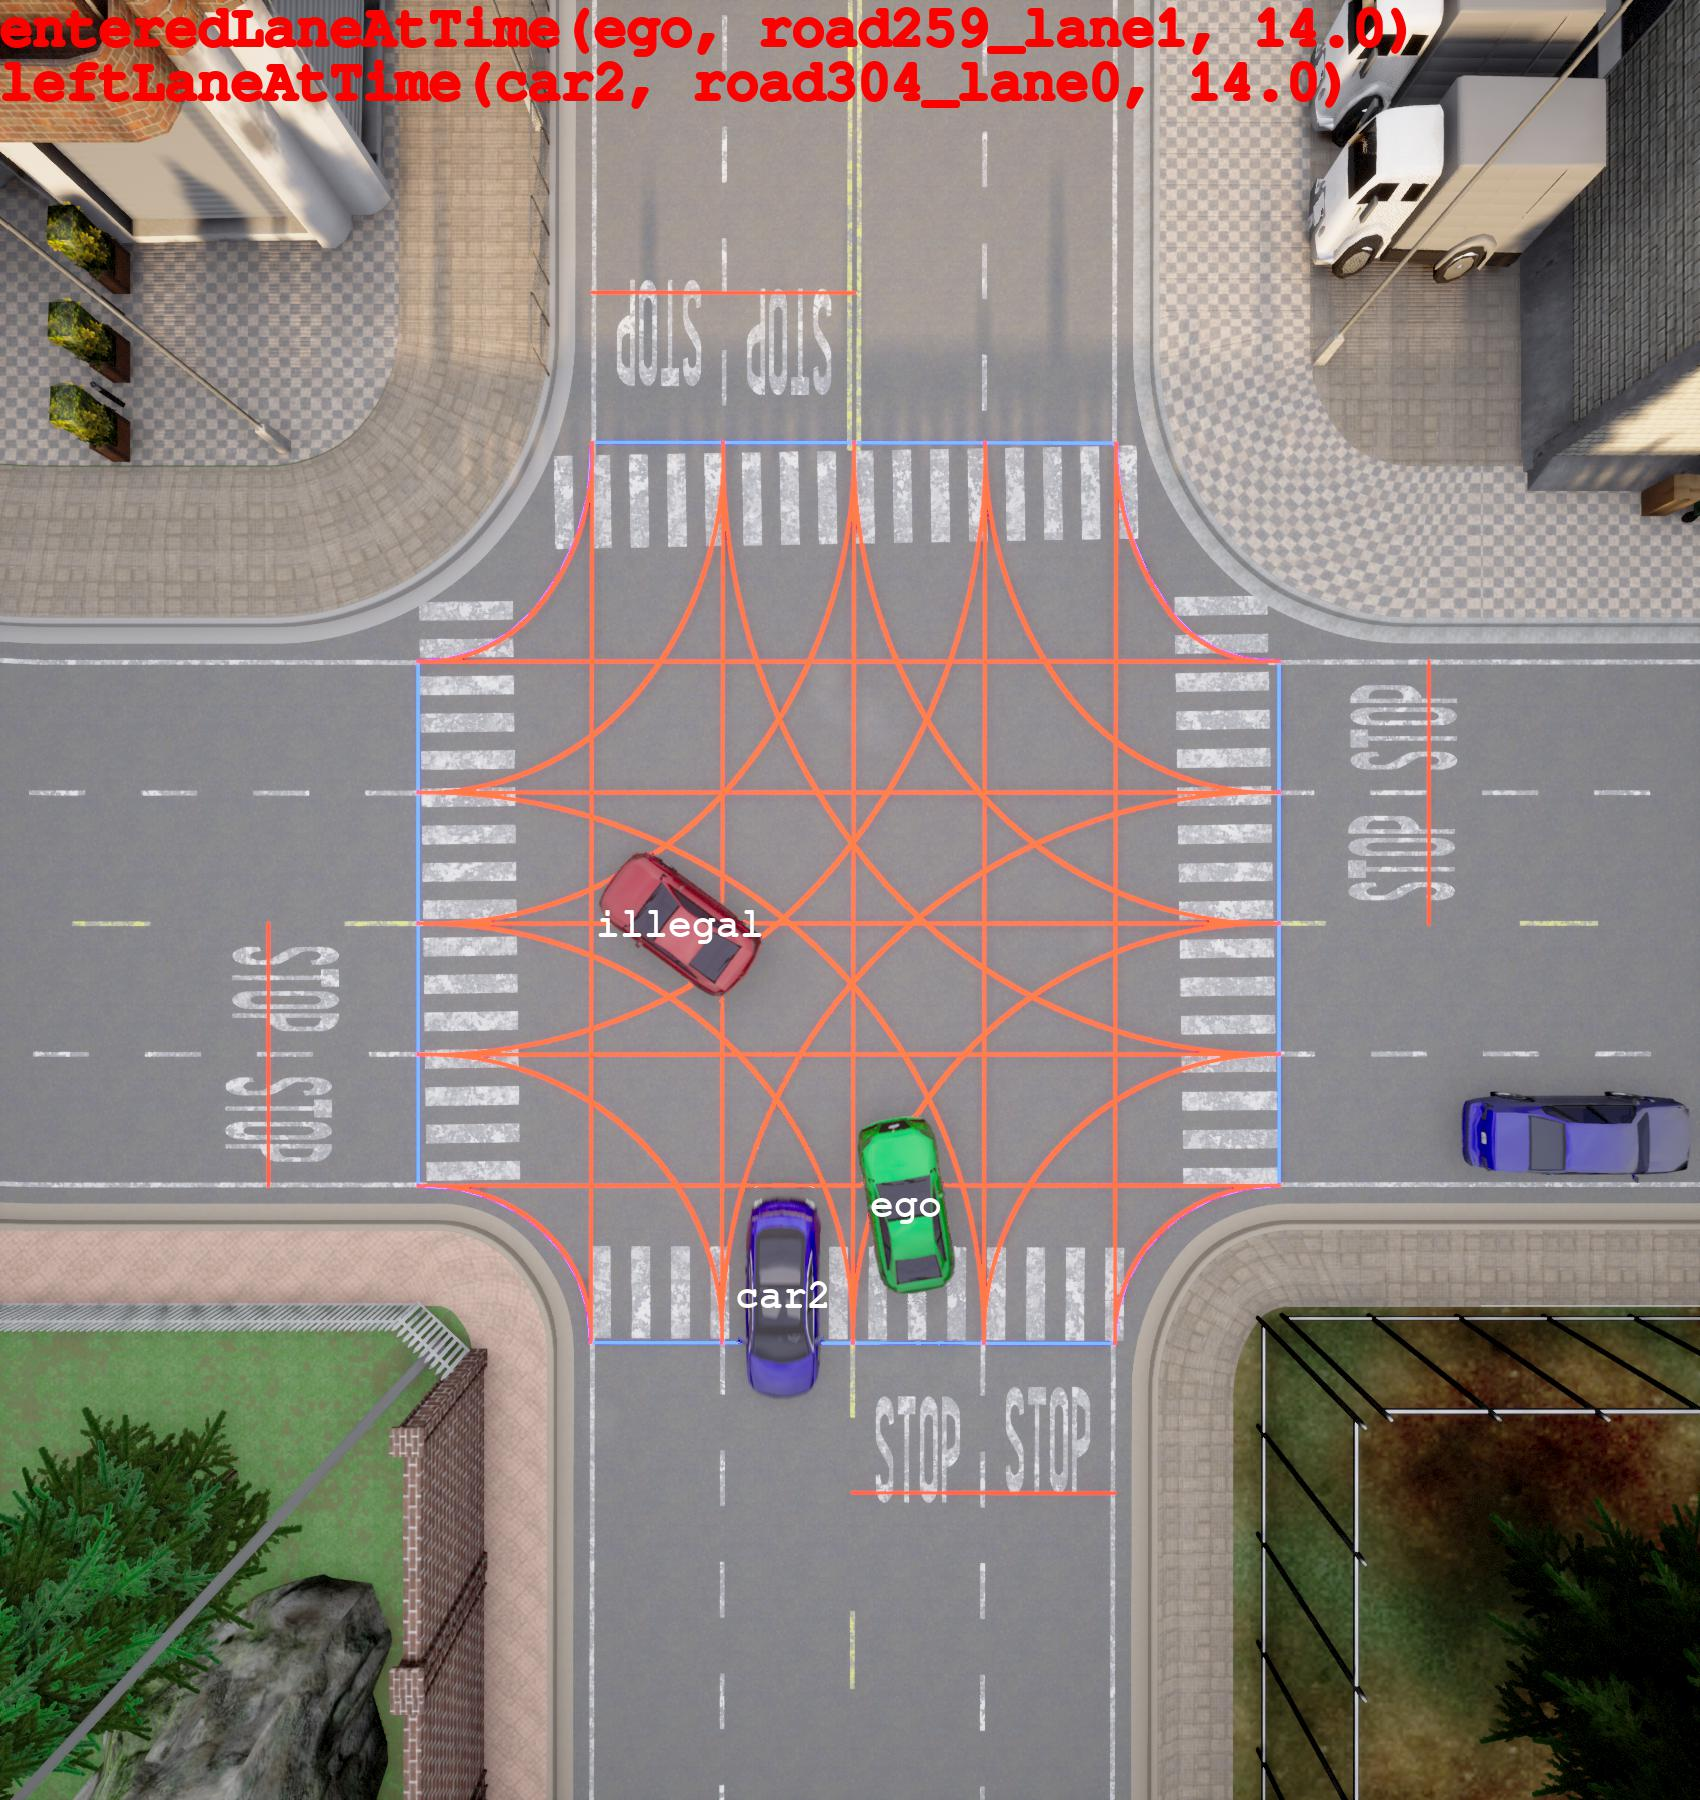
\includegraphics[width=\linewidth]{figures/chapter4/2_280.jpg}}%
    \subcaption{ego enters car2's route.}
  \end{minipage}%
  \caption{Left turn from a 4way-stop.}
  \label{fig:4way}%
\end{figure}% <<<

\textbf{Four-way Stop:} The first example demonstrates making incrementally more complex test-cases by adding more non-egos.
%
The goal of ego is to make a left turn from a four-way stop.
%
Ego starts from the bottom side of the intersection in Figure~\ref{fig:4way} and must exit the intersection from the left side.
%
We generate three test-cases, each more complex than the previous one.
%
In the first test-case a non-ego is added that enters the intersection from the left and passes straight through the intersection.
%
In the second test-case (visualized in Figure~\ref{fig:4way}), a non-ego is added that approaches from the top, the opposite side of ego, and passes straight through the intersection.
%
In the third test-case, a non-ego is added that approaches also from the left but the other lane of the road, and passes straight through the intersection.
%
Both CARLA's autopilot and autopilot-plus-RSS pass the first test-case.
%
Autopilot fails the second test-case while autopilot-plus-RSS passes it.
%
Finally, both autopilot and autopilot-plus-RSS fail the third test-case.
%
See the videos for even more complex extensions of this test-case.


%---------------------------------------
\begin{figure}% >>>
  \centering
  \begin{minipage}[t]{.499\linewidth}
    {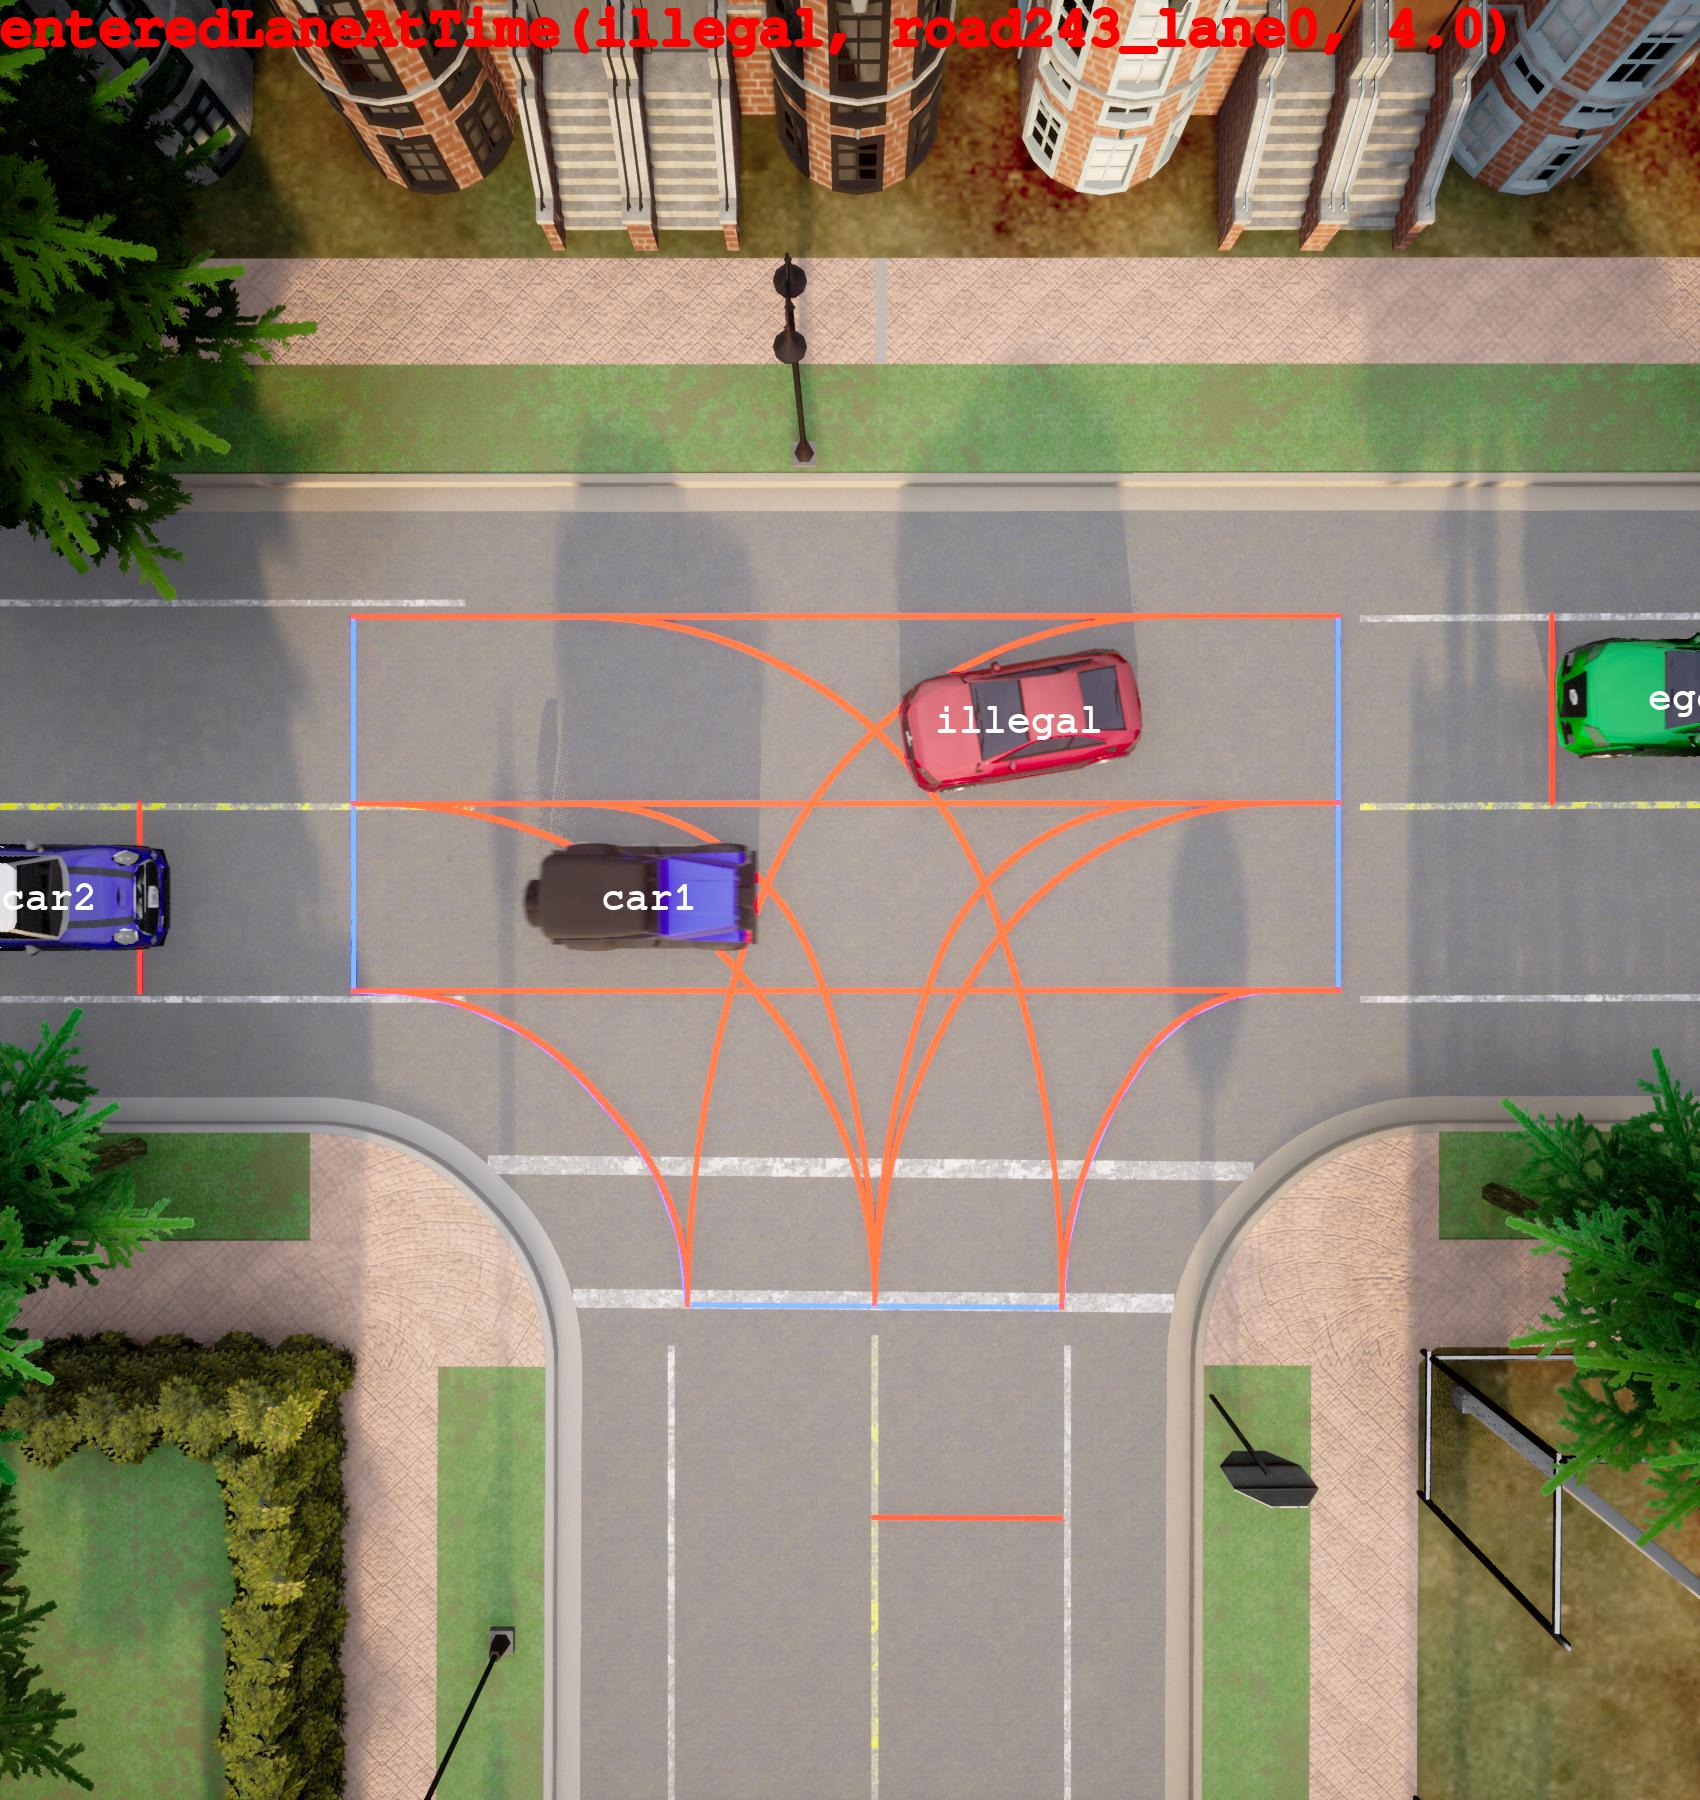
\includegraphics[width=\linewidth]{figures/chapter4/T-intersection/1_80.jpg}}%
    \subcaption{car2 approaches (passes the red line) before illegal enters car2's route}
  \end{minipage}%
  \hfill
  \begin{minipage}[t]{.499\linewidth}
    {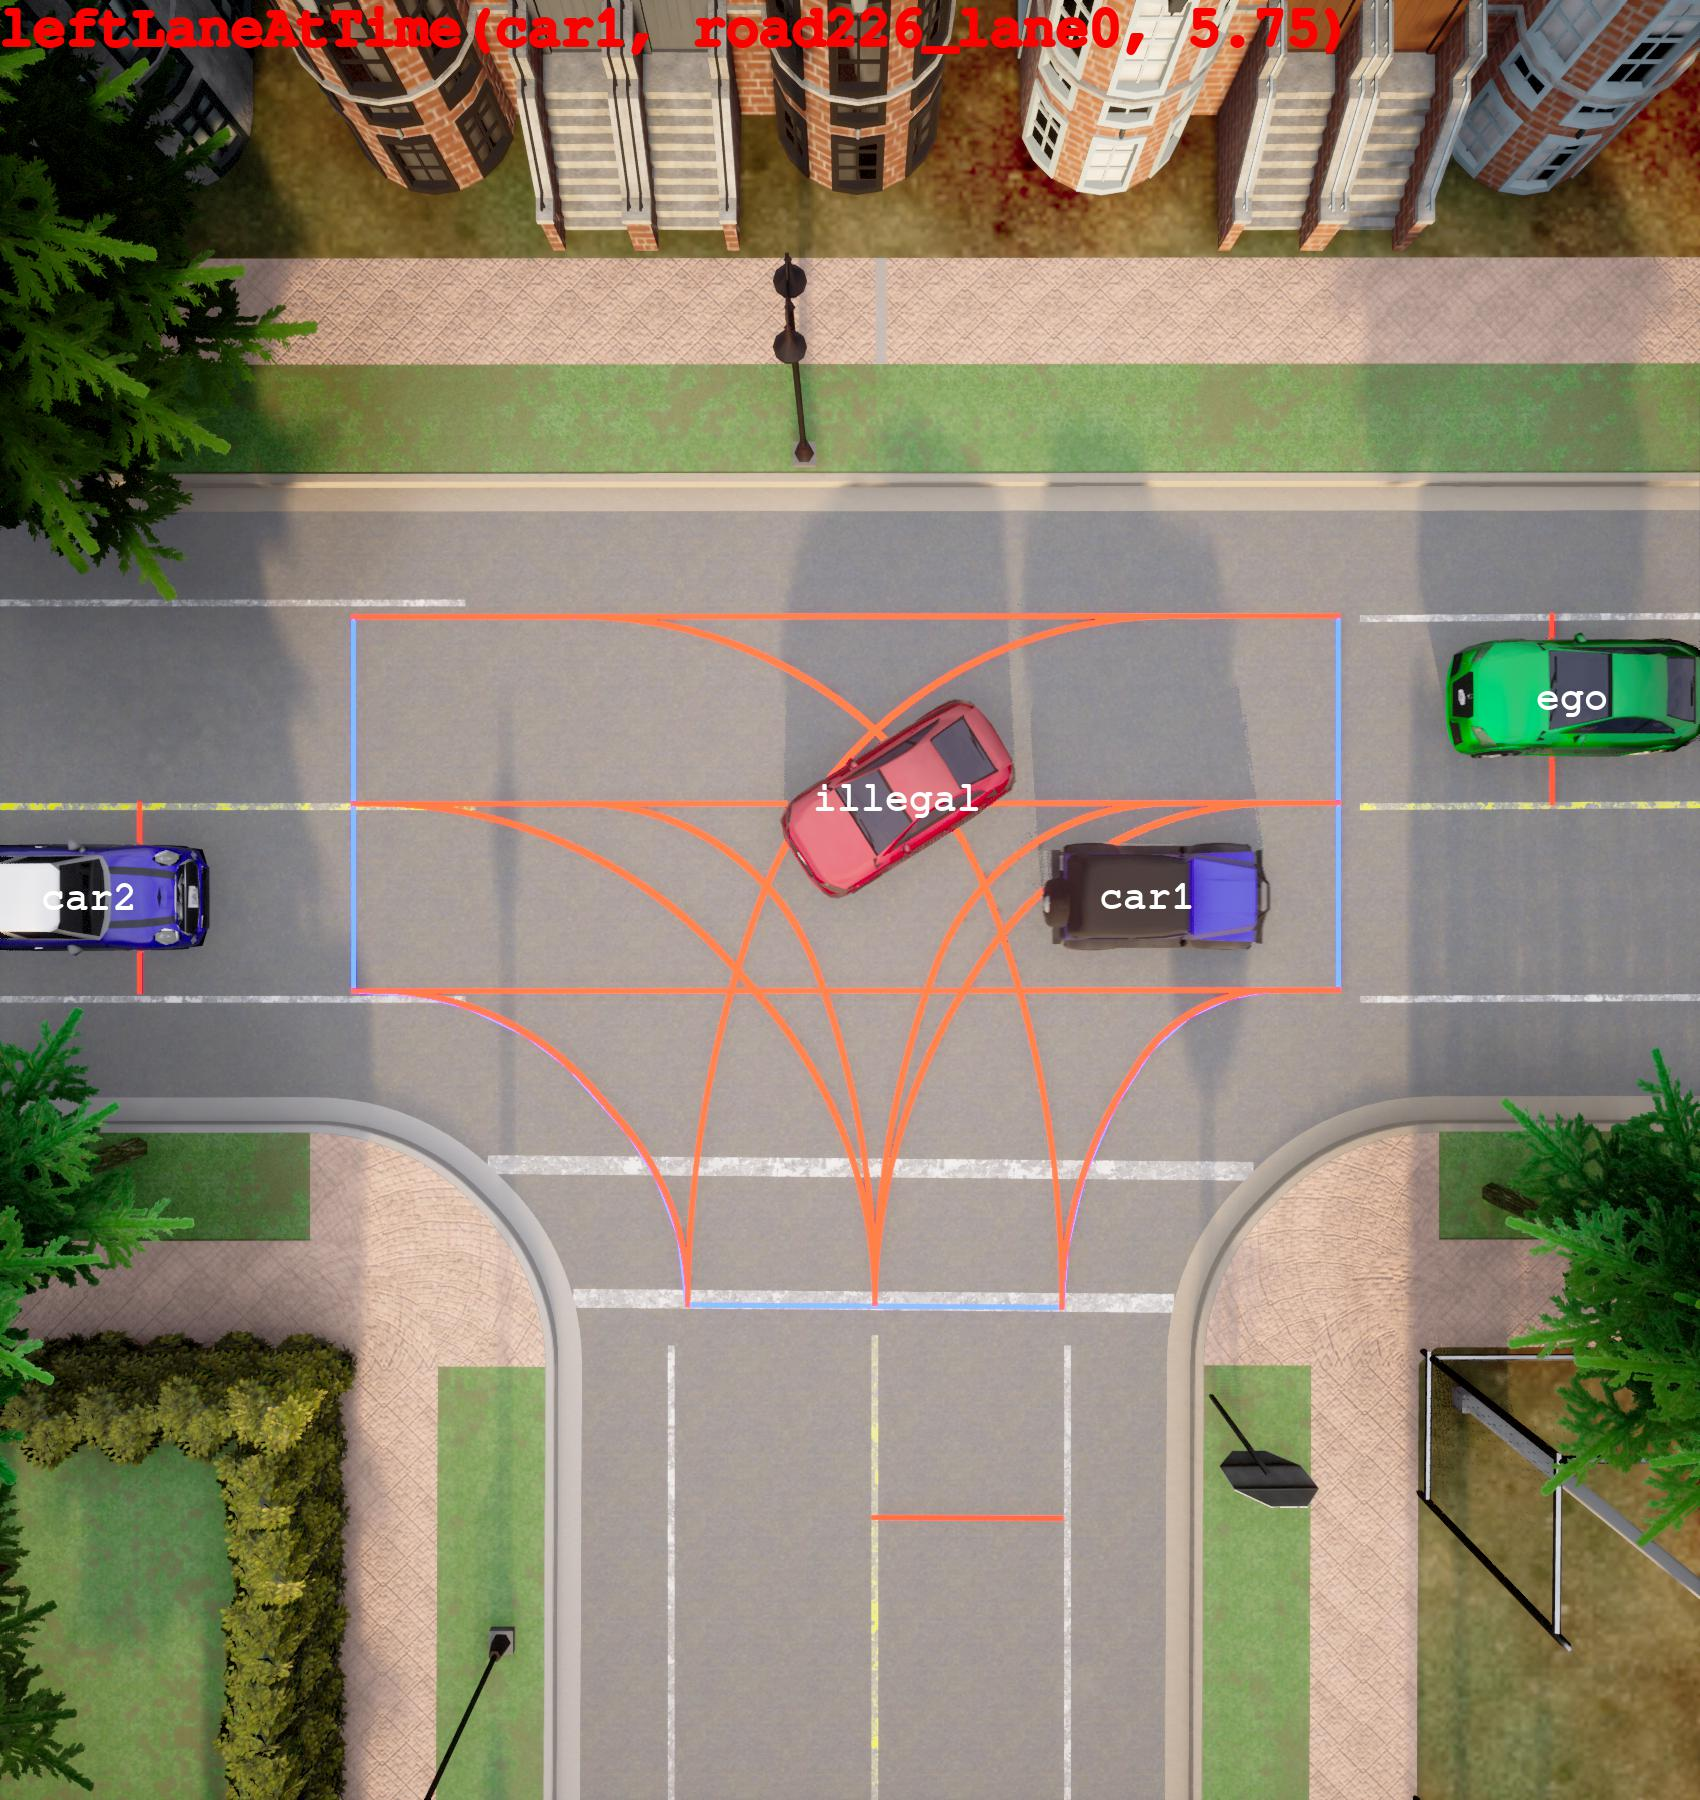
\includegraphics[width=\linewidth]{figures/chapter4/T-intersection/1_115.jpg}}%
    \subcaption{illegal does not yield to car2}
  \end{minipage}%
  \caption{Unprotected left turn from continuing highway.}\label{fig:continuing}%
\end{figure}% <<<


\textbf{T-intersection:} The goal of ego is to perform an unprotected left turn from the continuing highway to the terminating highway of the T-intersection shown in Figure \ref{fig:continuing}.
%
Ego approaches the intersection from the right side and must make a left turn to enter the road on the bottom.
%
This example demonstrates that we can add multiple non-egos to a test-case simultaneously.
%
Starting with an empty test-case, our test-case generator adds multiple non-egos that pass straight through the intersection from left to right.
%
CARLA's autopilot fails this test-case but autopilot-plus-RSS passes it.



%-------------------------------------------------------
\begin{figure}[ht]% >>>
  \centering
  \begin{minipage}[t]{.499\linewidth}
    {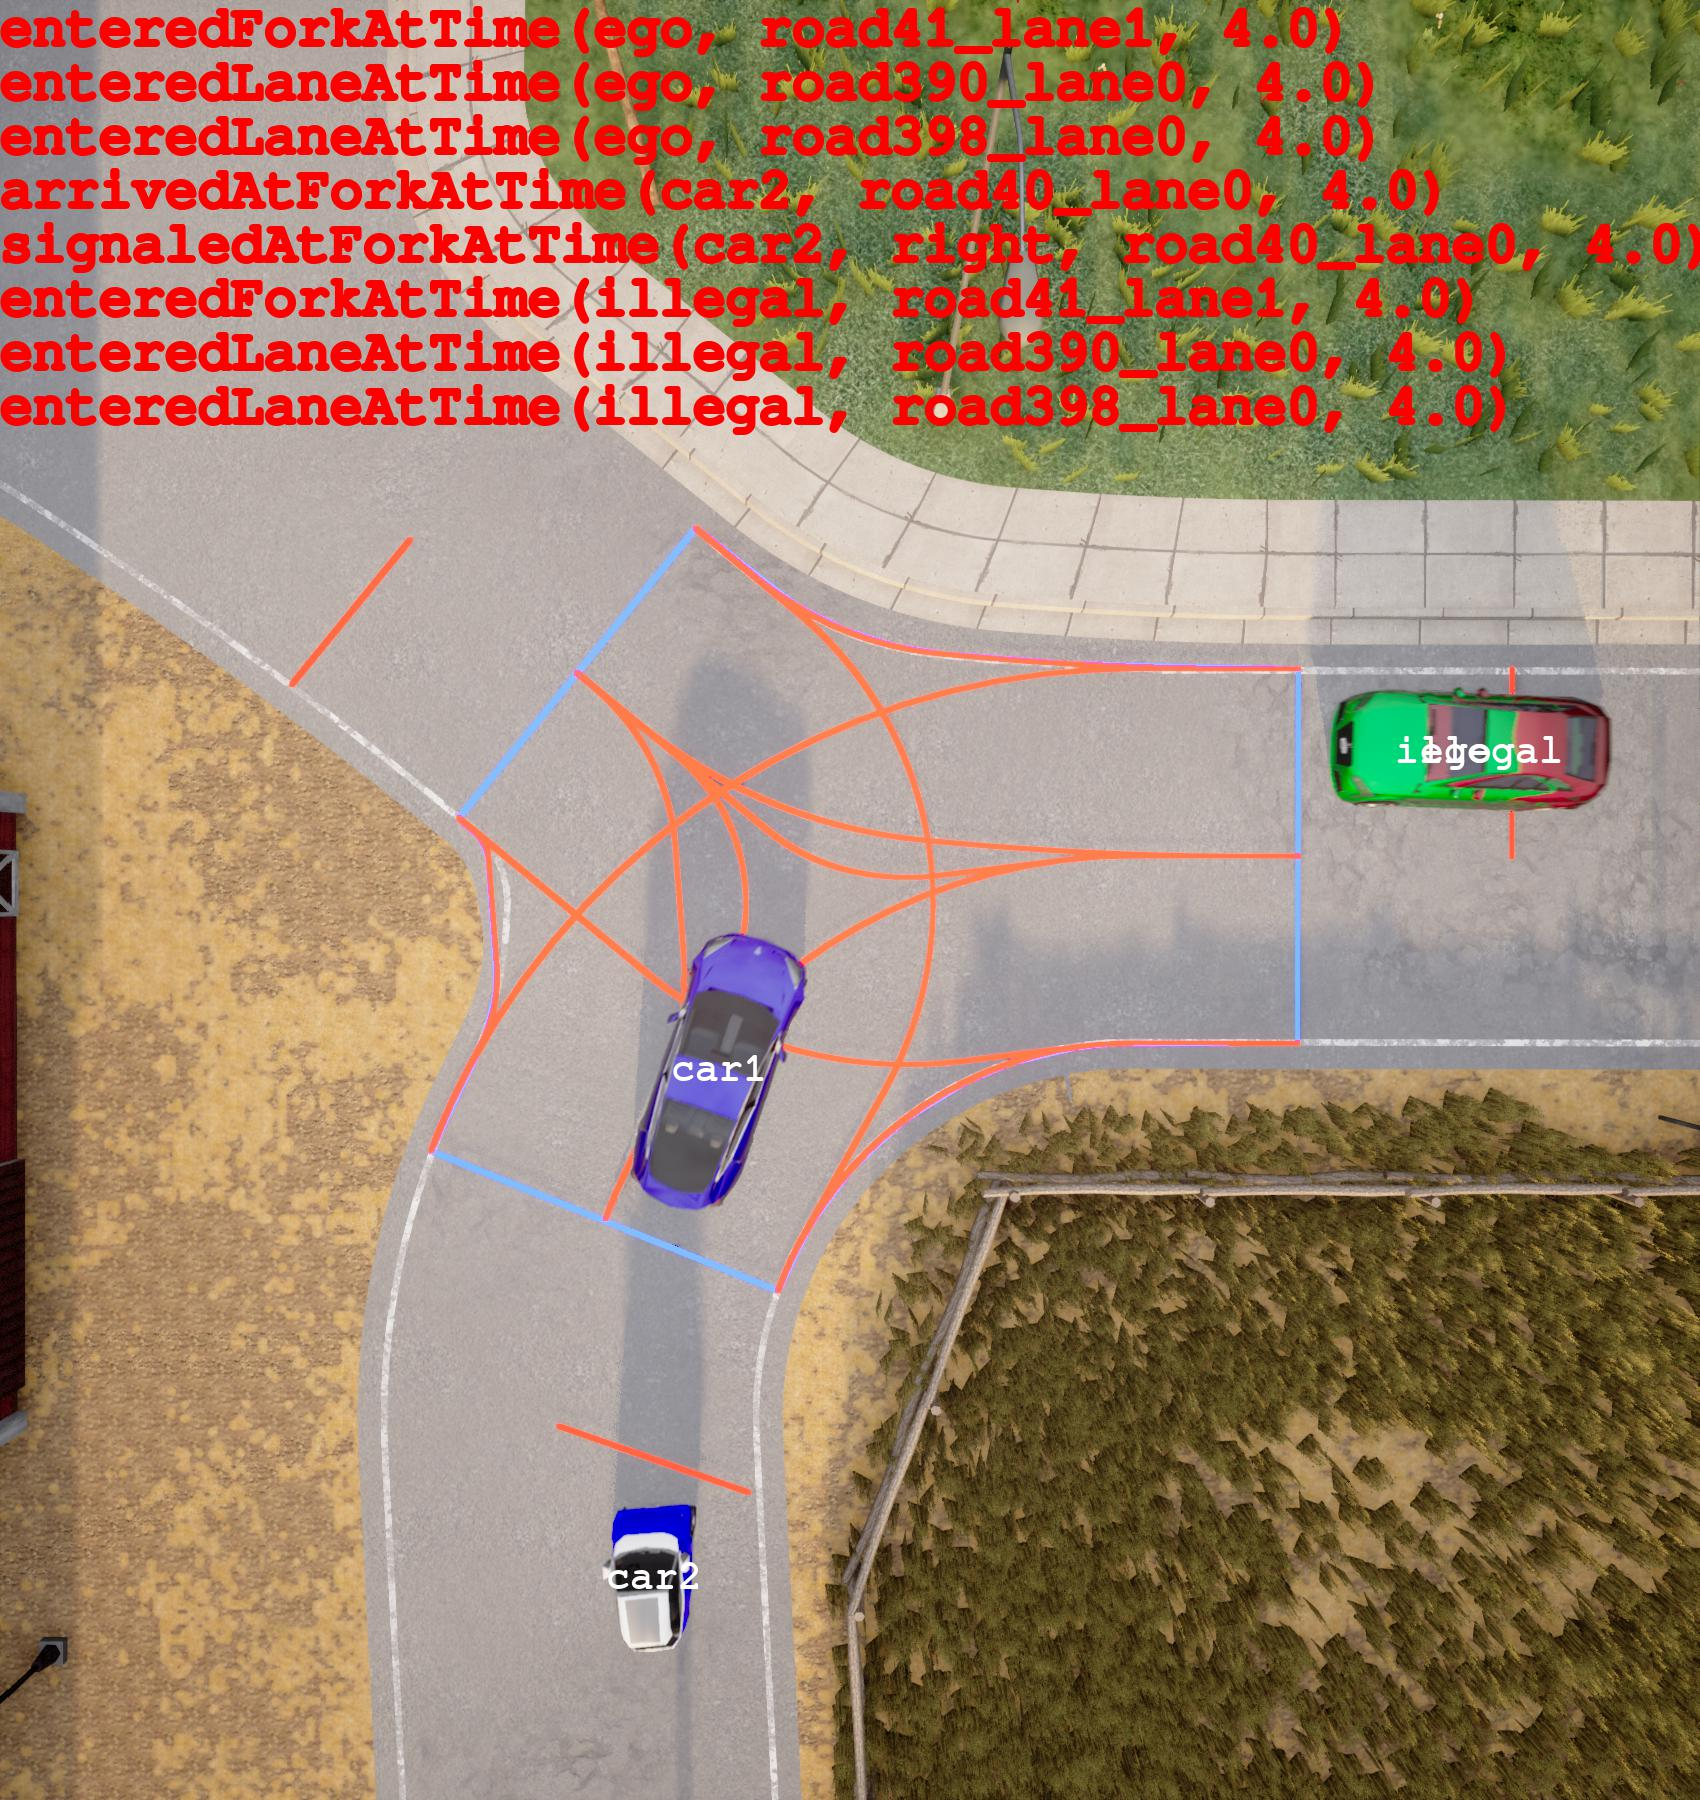
\includegraphics[width=\linewidth]{figures/chapter4/Y-intersection/1_80.jpg}}%
    \subcaption{car1 enters earlier than ego and illegal.}
  \end{minipage}%
  \hfill
  \begin{minipage}[t]{.499\linewidth}
    {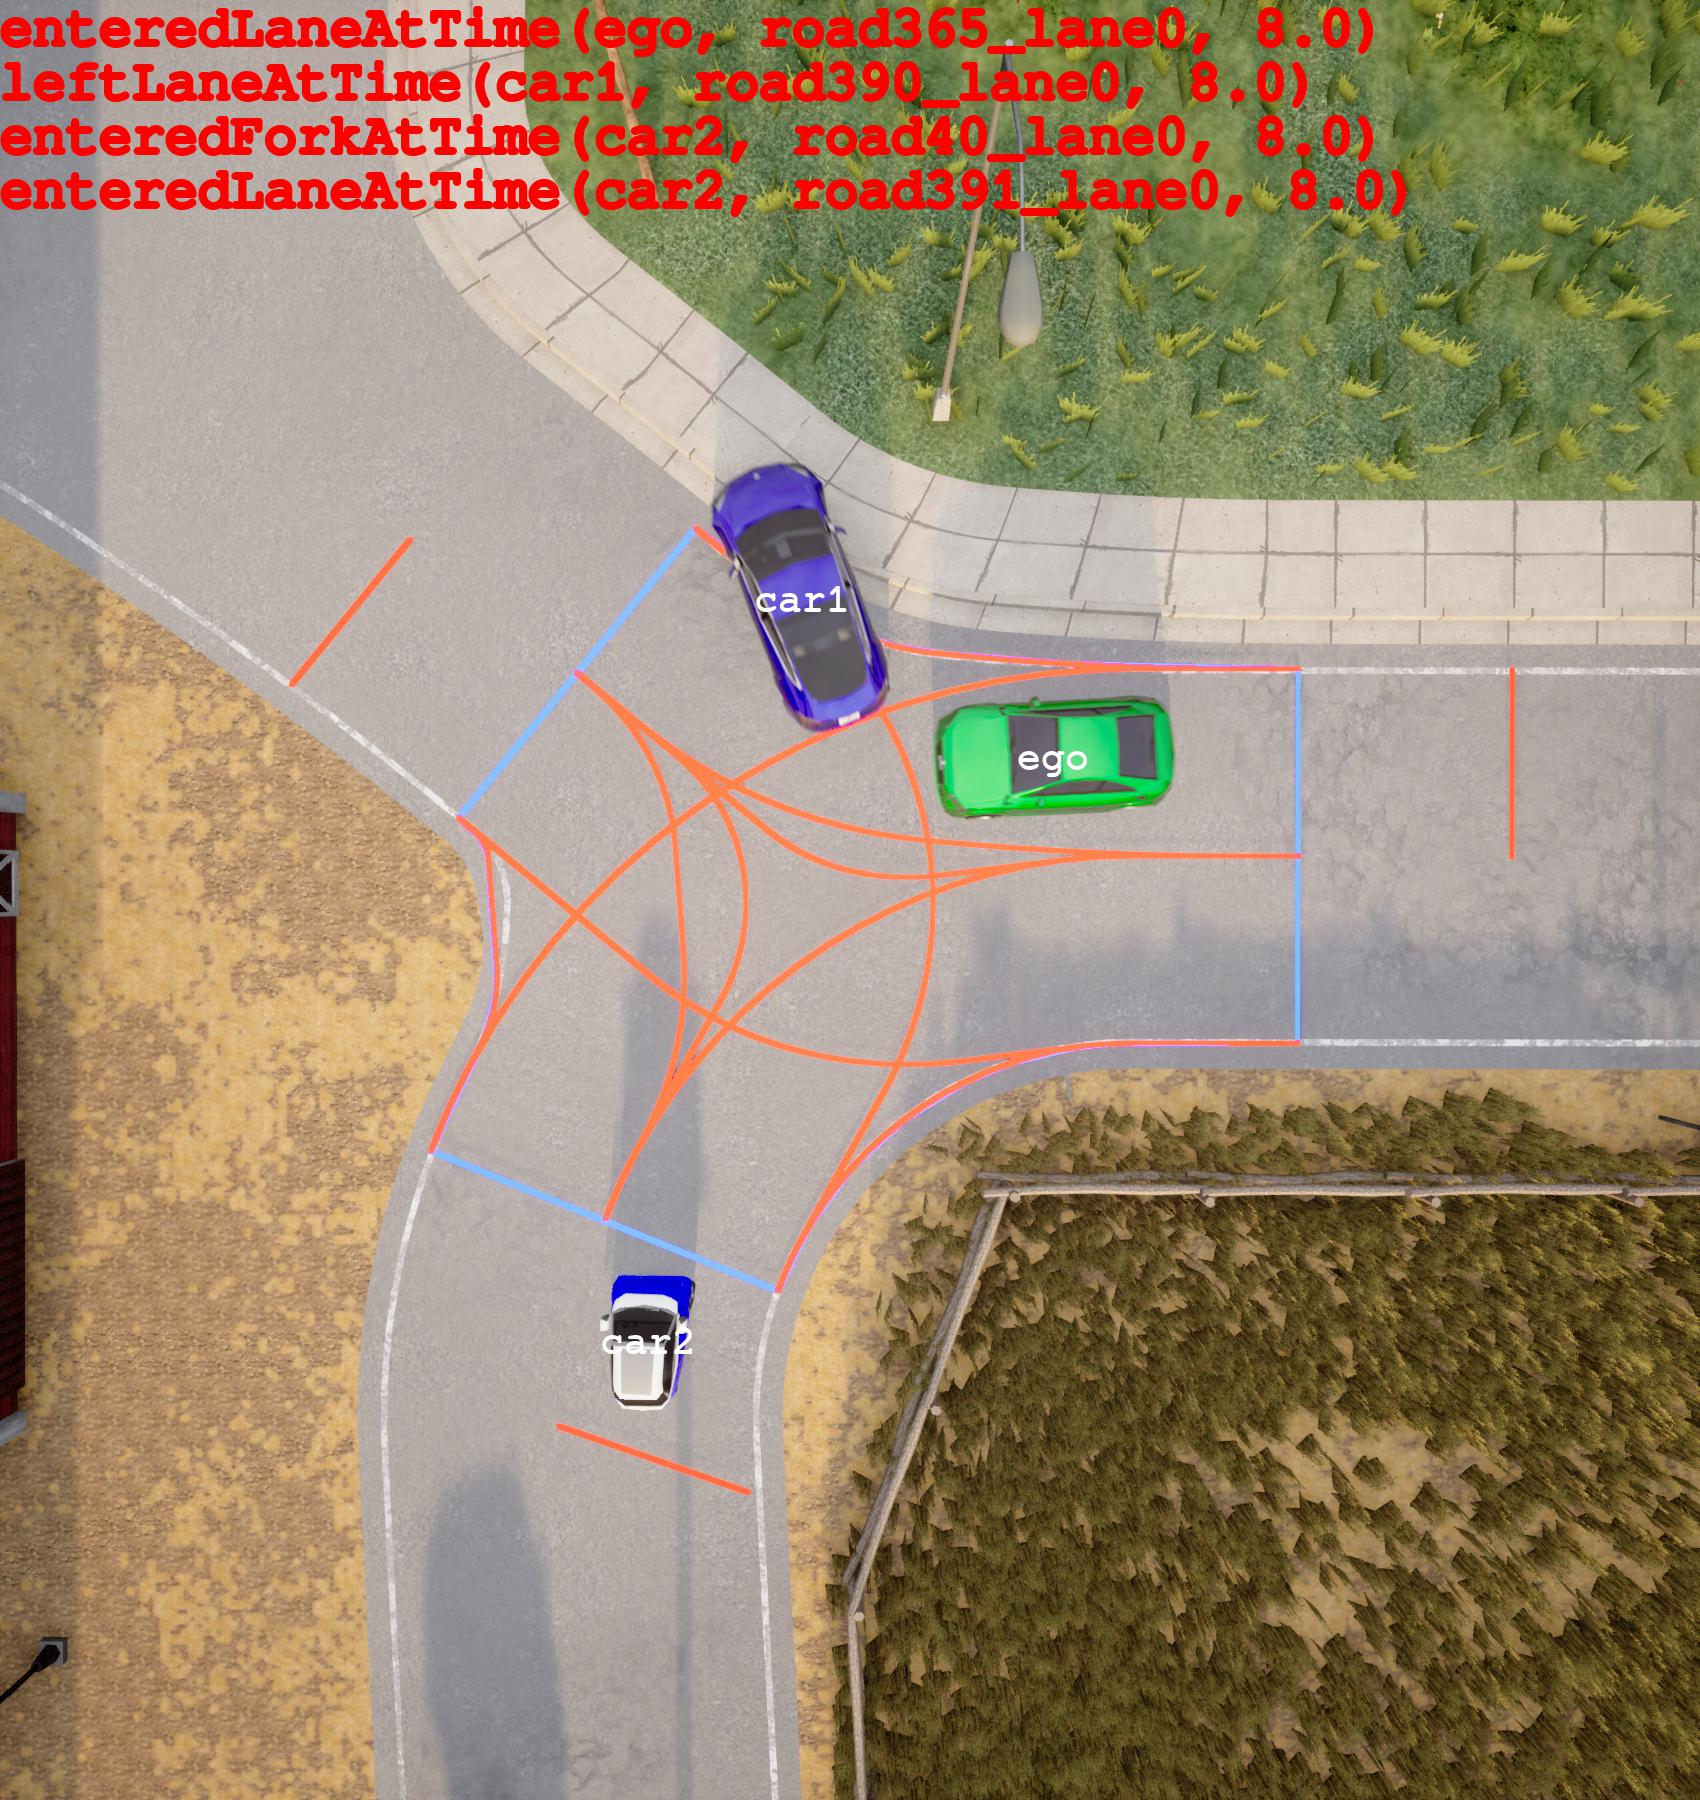
\includegraphics[width=\linewidth]{figures/chapter4/Y-intersection/1_160.jpg}}%
    \subcaption{illegal already exited from the bottom but ego waited for car1.}
  \end{minipage}%
  \caption{Unprotected left turn from an uncontrolled Y-intersection.}\label{fig:Y-intersection}%
\end{figure}% <<<


\textbf{Y-intersection:} The third example demonstrates that we can add a non-ego whose route does not conflict ego's route, as long as we add also a non-ego whose route has a conflict so that the test-case can become more complex.
%
Autopilot fails this test-case.
%
Running Autopilot-plus-RSS results in a segmentation fault which seems to be due to a bug in CARLA's map or integration of RSS.
%
Ego's goal is to approach from right and make a left turn to the bottom of the intersection.
%
The conflicting non-ego, {\verb car1 }, approaches from the bottom, makes a left turn and exits from the top left corner of the intersection.
%
The non-conflicting non-ego, {\verb car2 }, also approaches from the bottom, but makes a right turn and exits from the right side of the intersection.


\section{Related work}
In \cite{Xia.2017,Xia.2018,Gao.2019}, a \emph{complexity index} is defined based on some \emph{influence factors} and their relative importance.
%
The influence factors are based on the functionality of the AV that is going to be tested and may include a mixture of perception-related and planning-and-control-related factors such as weather, rapid changes in light, lane line clarity, road curvature, road congestion, etc.
%
These factors are derived from technical specifications, naturalistic traffic data, etc.
%
The contribution of each factor to the complexity index is derived with a quantitative and subjective evaluation, the Analytic Hierarchy Process (AHP).
%
In contrast to subjective assessments, we rely objectively on the pass-fail criteria alone to automatically decide if a test-case is more complex than another.
%
We give sufficient conditions that guarantee that a test-case $B$ is at least as complex as a test-case $A$, and a certificate to why $B$ is more complex than $A$.


%---scene complexity
Wang et al. \cite{Wang.2018} give a measure of complexity of scenarios gathered from an AV.
%
They first define a measure of scene complexity, then calculate its distribution across a scenario as a measure of its complexity.
%
That is, the spatio-temporal relations between two consecutive scenes are ignored.
%
Therefore, two scenarios with a completely different spatio-temporal development but the same distribution of scene complexity would be treated the same.
%
The \emph{scene complexity} is a weighted sum of \emph{road semantic complexity} and \emph{traffic element complexity}.
%
\emph{Road semantic descriptors} are features that are subjectively selected to contribute to the complexity measure, and obtained via manual annotations for a small subset of the data and generalized with supervised learning.
%
\emph{Traffic element complexity} is quantified in terms of non-egos' distance and orientation relative to the AV (ego), which makes their definition fall under criticality rather than complexity in our terminology above (adopted from \cite{Riedmaier.2020}).


Qi et al. \cite{Qi.2019} propose a manual process to characterize a test-case based on a finite number of failing trajectories of ego.
%
The causes of failure are analyzed to make a list of Scenario Character Parameters (SCPs) which could be related to perception, planning or control aspect of the driving task.
%
In contrast, our characterization of a test-case is with respect to all (infinitely many) failing ego behaviors.
%
Furthermore, our algorithm decides the cause of failure of a behavior automatically from the pass-fail criteria.

%---Scenario generation methods
Apart from a few papers reviewed above that generate complex test-case scenarios, most literature on scenario generation/selection focus on other qualities and quantities of scenarios, such as \emph{similarity} \cite{Harder.2021}, \emph{criticality} \cite{Klischat.2019,Zhong.2021}, \emph{corner cases} \cite{OKelly.2018}, etc.
%
These techniques include a variety of algorithmic paradigms such as  knowledge-based methods \cite{Li.2020}, data-driven methods \cite{OKelly.2018}, optimization-based search \cite{Klischat.2020,Feng_Methodology.2020,Feng_CaseStudies.2020}, genetic algorithms \cite{Klischat.2019,Calo.2020,Zhong.2021}, synthesis from formal specification \cite{Klischat.2020,Tuncali.2019}, probabilistic search \cite{Fremont_testing.2020,Tuncali.2016}, combinatorial search \cite{Tuncali.2019,Gao.2019,Xia.2018}, etc.
%
Only a few of the proposed techniques handle traffic rules, especially right-of-way, at intersections.
%
In a survey on performing safety assessment of autonomous vehicles~\cite{Riedmaier.2020}, the authors stress the importance of scenario generation at intersections.
%
Here, we mention a few examples that are more related to our work.


%---probabilistic programming
Fremont et al. \cite{Fremont_testing.2020} use Scenic as a probabilistic programming DSL to generate scenarios.
%
In contrast, we use Scenic only as an interface to CARLA, and generate the scenarios by solving logic programs.
%
An advantage of logic programming over probabilistic programming is that a logic solver gives coverage guarantee over its search space.
%
For example, in Step 2 of our algorithm, the ASP solver covers all possible order relations between events, where ASP's search space is restricted by the order relations that are fixed in Step 1.


%---intersections
Tuncali et al. \cite{Tuncali.2019}, also Klischat and Althoff \cite{Klischat.2020} generate test-cases for intersections from requirements and formal specifications.
%
However, they do not include right-of-way traffic rules.


%---solvability and complexity certificates
Calo et al. \cite{Calo.2020} use genetic algorithms to find \emph{avoidable collision scenarios}.
%
These are scenarios in which a particular AV crashes but it could have avoided the collision.
%
This is somewhat similar to our complexity and solvability certificates: a behavior that fails a test-case and a behavior that passes the same test-case.
%
However, our goal is different, i.e. finding a test-case that is more complex than a given test-case.
%
Also, our pass-fail criteria are not limited to collisions.


%---synthesis using SMT
In \cite{kim2019test} SMT solving is used to generate test-cases.
%
To generate trajectories, they use a predetermined geometric class, say piecewise linear or spline curve. 
%
Therefore, the generated trajectory is not necessarily feasible for the steering geometry of a vehicle, say with Ackermann steering.
%
In contrast, we satisfy the steering constraints using simulation and closed-loop control, and use SMT only for generating the longitudinal speed.



\chapter[~~~~~~~~~~~~Predicate-Coverage-Guided Fuzzing]{Predicate-Coverage-Guided Fuzzing}
\label{ch:fuzzing}

\section{Introduction}

Fuzz testing (or fuzzing) is one of the widely used tools for automatic test case generation.
% 
It has received a lot of attention, particularly from the security community to search for exploits and is now part of standard testing procedures for any security-critical project.
% 
For determining security exploits, people often use \emph{goal driven fuzzing}.
% 
However, for assessing various factors such as code quality, path coverage, dead code detection, etc, coverage-driven fuzzing is widely employed.

\begin{figure}[t]
    \centering
    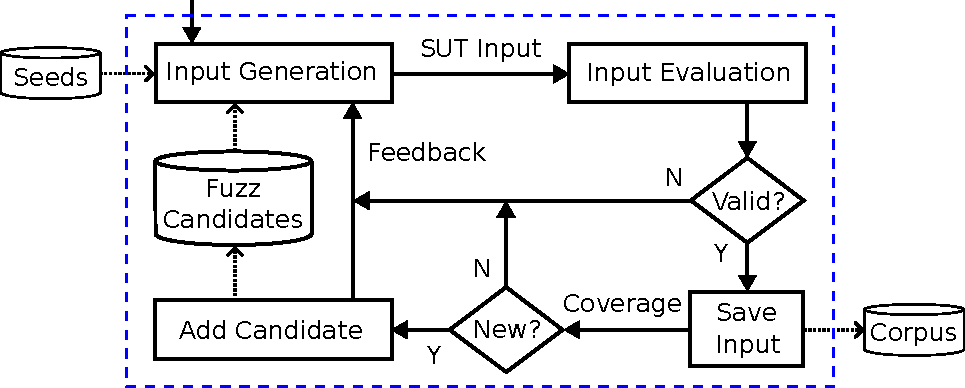
\includegraphics[width=0.9\linewidth]{figures/chapter5/Coverage-Guided Fuzzing.pdf}
    \caption{Coverage-Guided Fuzzing}
    \label{fig:fuzzing}
\end{figure}

The overall workflow of a fuzzing technique is given in Figure~\ref{fig:fuzzing}.
% 
The system under test is first tested with some set of random test inputs or a test suite that is manually generated.
% 
The outcomes of these test inputs, for example, coverage metrics like code coverage, or branch coverage are then evaluated and stored as test outputs.
% 
The coverage driven fuzzer assesses the various outputs of the inputs and selects a specific subset of tests to be added to seed collection.
% 
The fuzzer then assigns potential function to each of the seeds and generates a new test input by applying one of the mutator functions that can be either specified by the user or standard mutators that are available in the library.


In the case of AVs navigating through intersections, we automatically generate the behavior of all the non-ego vehicles.
% 
This includes generating the velocity profiles, the entry and exit lanes, and the turn indicators of all the vehicles.
% 
Based on the formalization of traffic rules, we then collect all the predicates that are triggered by the behavior of both the AV and the non-ego vehicles.
% 
Given a specific test scenario, the fuzzer asssess the importance of a given test input based on the new collection of predicates that are triggered by it.
% 
The mutators that change the given test scenario change 1) the entry and exit lanes of non-ego vehicles, 2) the velocity profile of the vehicles, and 3) the various turn signals associated with each behavior.
% 


\section{Evaluation}

Our goal of fuzzing for scenario generation is to generate a set of diverse test scenarios for various autonomous agents as efficiently as possible.
% 
To answer this question, the evaluation is divided into two parts.
% 
First part deals with effectiveness and efficiency of fuzzing operations.
% 
This evaluation quantifies whether fuzzing actually generates better coverage than pure random testing.
% 

The second part tries to generalize the test cases covered for one agent can be applied to another agent.
% 
Given the wide variety of ego agents, at least 10 different companies working on AV logic, it is unclear if generating fuzzing inputs for one agent would result in the same coverage for other agents.


\subsection{Evaluation Guidelines}
Kleese et al. \cite{Klees.2018} conclude several good/necessary practices for experimental evaluation of fuzzers.
%
We summarize the main points and try to follow their advice in our evaluation.
%
First, the relative performance between two fuzzers can change over time, so shorter experiments have higher risk of showing misleading results.
%
Second, multiple trials should be done for statistical validity.
%
Finally, due diligence must be made in reporting the details of evaluation, which helps with reproducibility of the results.
%
For example, one should clearly report the performance measures used, the baselines, fuzz targets, fuzzer parameters such as seeds and timeout, the number of trials, and the statistics used to analyze/summarize the results.


Herrera et al. \cite{Herrera.2021} investigate the role of seeds in fuzzing performance and give advice on comparing fuzzers.
%
They conclude that the choice of seeds can have a significant impact on a fuzzer's performance, so it should be clearly documented in an experimental evaluation.
%
Also, one should never use only a single seed.


The recent reproducibility crisis \cite{Baker.2016}, \cite{Oza.2023} in the sciences have highlighted some questionable scientific experiment practices.
%
We are aware of some of these problems which are rooted in frequentist statistics \cite{Jaynes.2003}, \cite{Clayton.2021}.
%
As such, we intentionally did not perform any statistical tests since we are not sure which bayesian method would be informative to summarize our results.
\subsection{Evaluation Set-up}

% \begin{figure}
%     \centering
%     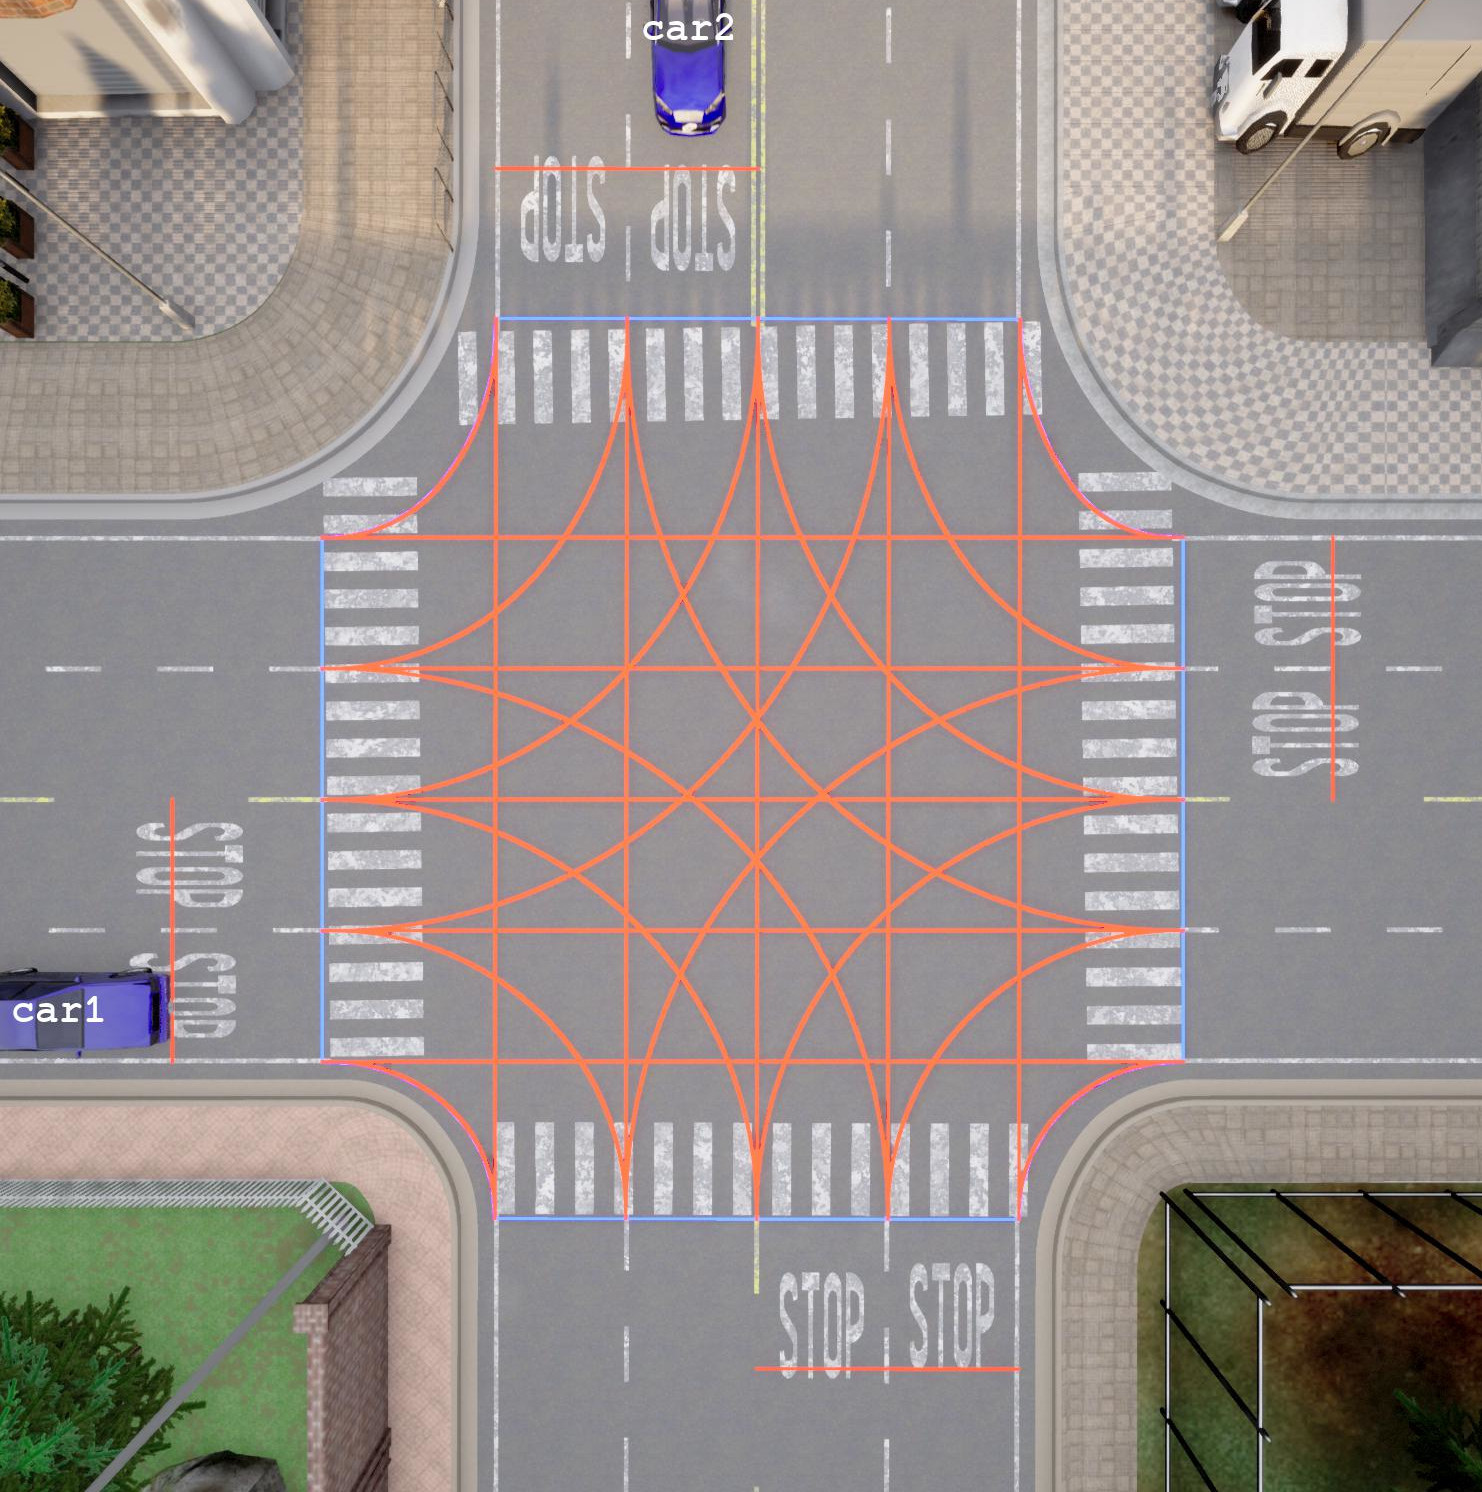
\includegraphics[width=50mm]{figures/4way-stopOnAll.jpg}
%     \caption{Multi-lane four-way stop}
%     \label{fig:4way-stopOnAll}
% \end{figure}

For evaluating the effectiveness of fuzzing in generating a diverse set of inputs, we consider a multi-lane four-way intersection, with two incoming lanes and two outgoing lanes from each side, such as the one provided in Figure~\ref{fig:4way-stopOnAll}.
% 
Considering that a scenario can have several cars waiting to enter and exit the intersection at different points of time, one can think of various scenarios.
% 
Each scenario can have at most one ego vehicle (that implements autonomous driving software) and several non-ego vehicles whose trajectories are generated algorithmically.
% 
The number of non-ego vehicles, the path prescribed to each non-ego, and the velocity profile of each non-ego vehicle is generated by the fuzzer.
% 
As mentioned earlier, since bit-level fuzzing of a scenario description most likely does not yield in a new valid scenario, we use structure-aware fuzzing where we provide custom mutators for manipulating vehicle routes, velocity profiles, etc.
% 
Once the fuzzing algorithm generates a scenario, the scenario is evaluated in a photo-realistic simulator such as CARLA.
% 
We collect the valuations of all the predicates during the scenario to calculate its predicate coverage.
% 
\emph{The predicate coverage metric is the number of unique predicate valuations.}
% 

% The predicates encountered by the ego-vehicle while navigated through the scenario are recorded and used for evaluating the predicate coverage.

%------------------------------------------------------
\subsubsection{Scenario Encoding}
A \emph{test-case scenario} consists of one or more \emph{non-ego} vehicles, and an \emph{ego} vehicle.
%
The trajectories of non-ego vehicles are predetermined at test-case generation time.
%
A test-case specifies the initial position of the ego vehicle while the rest of the trajectory is generated at test-case execution time when an ego \emph{agent} drives the ego vehicle.
%
The ego vehicle is expected to follow a \emph{route} as specified by the test-case, also called ego's \emph{mission}.
%
Each vehicle is associated with a vehicle model, which specifies its shape and dynamics.
%
Each non-ego trajectory is specified using two polynomial splines: \emph{footprint} and \emph{timing}.
%
A \emph{footprint} spline specifies the positions of a vehicle parameterized by travelled distance.
%
The \emph{timing} spline specifies the travelled distance of a vehicle parameterized by simulation time.
%
The \emph{local control property} of splines allows mutators to change a trajectory locally (in location or time) by mutating the splines' control points.
%
This allows local search in the space of trajectories, which is the motivation behind our scenario encoding design.
%
A test-case also specifies the turn-signal events of each non-ego, as a list of pairs of (time, turn signal).


%------------------------------------------------------
\subsubsection{Seeds}

The initial fuzzing seeds are randomly sampled using a probabilistic programming language called SCENIC \cite{Fremont.2020}.
%
A SCENIC scenario specifies a distribution over scenarios, and SCENIC's generator samples from this distribution.
%
The number of vehicles and their initial positions are first sampled to create an \emph{initial scene}.
%
Then each vehicle is driven by an agent to generate vehicle trajectories.
%
One of the vehicles is designated as the ego vehicle.
%
The trajectories of non-ego vehicles are converted to our spline encoding using SciPy's spline approximation.
%
The trajectory of the ego vehicle is used to assign ego's route (mission), i.e. the expected lanes to follow.
%
We keep sampling from the SCENIC scenario for 20 minutes, resulting in 22 seeds.

%-----------------------------------------
\subsubsection{Mutators}
Since a traffic scenario is highly structured and constrained, we use structure-aware mutators.
%
That is, instead of mutating the bit-level representation of a fuzz-input,
the python-object representation of a test-case scenario is mutated such that
the mutant is still a valid python object of the same type.
%
We implemented the following mutators:
\begin{itemize}
    \item Copy/Move a vehicle (and its trajectory) along its route forward/backward.
    \item Copy/Move a vehicle (and its trajectory) to a different route. The local coordinates of the trajectory remains the same from the source route to the destination route (curvilinear frames).
    \item Remove a vehicle.
    \item Speed-up/Slow-down a vehicle by a random factor over a random time interval.
    \item Mutate ego’s route.
    \item Add/Remove a turn-signal event randomly.
\end{itemize}
%
In each fuzzing step we apply a random number of the above mutations to yield a new input for evaluation.


%-----------------------------------------
\subsubsection{Computation Budget}
For repeatability, we seed the pseudo-random number generators (PRNGs) before starting experiment.
%
For statistical validity, each experiment is tried 10 times, where each trial is run with a different PRNG seed.
%
We run all the experiments on a SLURM-managed HPC cluster.
%
Each fuzzing campaign is run for 24 hours.
%
We allocate 100GB memory and 8 CPUs for each trial.
%
For experiments that need a GPU (for the simulator or the ego agent),
we allocate a single NVIDIA Tesla V100 16GB SXM2.
%
The experiments in which the SCENIC agent drives the ego vehicle, a GPU is not needed.

\section{Evaluation Results}

\subsection{RQ1: Is code-coverage an efficient guide for generating diverse traffic scenarios?}

The main goal of this paper is to increase the diversity of scenarios encountered by an AV while navigating scenarios.
% 
Our primary hypothesis is that code-coverage is not an optimal feedback for guiding a fuzzer for this purpose.
%
The rationale 
%
This is important because off-the-shelf fuzzers use code-coverage for feedback and don't support user-defined coverage criteria.
%
To support our hypothesis, we develop our own fuzzer to show that improvement in test-case diversity can be achieved by using a more appropriate feedback.
%
We hope that our results encourage development of more flexible fuzzers to expand the reach and utility of this successful search technique.


%---------------------
\subsubsection{Performance Metrics}
We use two different metrics to compare our fuzzing technique with the baselines.
%
First, we use the total number of predicate valuations found per wall-clock time.
%
A predicate valuation can be represented as the set of predicates that evaluate to True.
%
Second, we use the total number of predicate-sets found per valid fuzz inputs found per wall-clock time.
%
The motivation behind the second metric is that test-case execution is expensive, so it's better to achieve the same coverage with less number of inputs.
%
This is the same idea behind \emph{corpus minimization} in fuzzing.
%
Nevertheless, the first metric is more important than the second one.


%---------------------
\subsubsection{Baselines}
The first baseline is a random fuzzer.
%
That is, at each fuzzing step, a fuzz-candidate is selected uniformly randomly.
%
The selected candidate is then mutated with the structure-aware mutators and then passed to input evaluation.


The second baseline, \emph{Atheris}, is a code-coverage-guided fuzzer.
%
Atheris supports fuzzing python programs, and is based on libfuzzer under the hood.
%
We configure Atheris to use our structure-aware mutators.
%
Libfuzzer, and so Atheris, use the Entropic power schedule.


%---------------------
\subsubsection{Our Fuzzer}
Our fuzzer uses the structure-aware mutators, similar to the baselines.
%
It also uses the Entropic power schedule, similar to Atheris.
%
We implemented Entropic in python by translating libfuzzer's C++ source code.
%
However, our Entropic implementation does not consider the size of fuzz-inputs, so it does not replace a fuzz-candidate with a smaller new one that has the same coverage.
%
Our fuzzer uses predicate-set coverage feedback to decide whether to add a mutant to the fuzz-candidates, and for calculating the energy of the fuzz-candidates.
%
In the following we refer to this fuzzer as PCGF-Entropic, for Predicate-Coverage-Guided Fuzzer with the Entropic power schedule.


%---------------------
\subsubsection{Trials}
We compare our fuzzer against the baselines for four different ego agents.
%
For each choice of ego agent, the experiment is repeated for 10 trials, each trial with a different PRNG seed from the set $\{ 0, \dots, 9 \}$.
%
We chose the following agents since they are all compatible with our SCENIC-CARLA simulation platform:
\begin{itemize}
    \item TF++.
        Trans-Fuser Plus Plus \cite{Jaeger.2023} is one of the top agents in CARLA Leaderboard 2.0.
        %
        We run the SENSORS Track version of the agent.
    \item CARLA Autopilot.
        This is a privileged agent controlled by CARLA's traffic manager.
    \item CARLA BehaviorAgent.
        This is a rule-based agent example provided by CARLA which demonstrates how to use CARLA's interface to implement custom agents.
    \item SCENIC agent.
        This is a rule-based agent implemented in the SCENIC language.
        %
        This agent is run using SCENIC's built-in NewtonianSimulator which only simulates the dynamics of vehicles based on a bicycle model.
        %
        The agent is controlled by SCENIC's path-following PID controllers for lateral and longitudinal control.
\end{itemize}


\begin{figure}
    \centering
    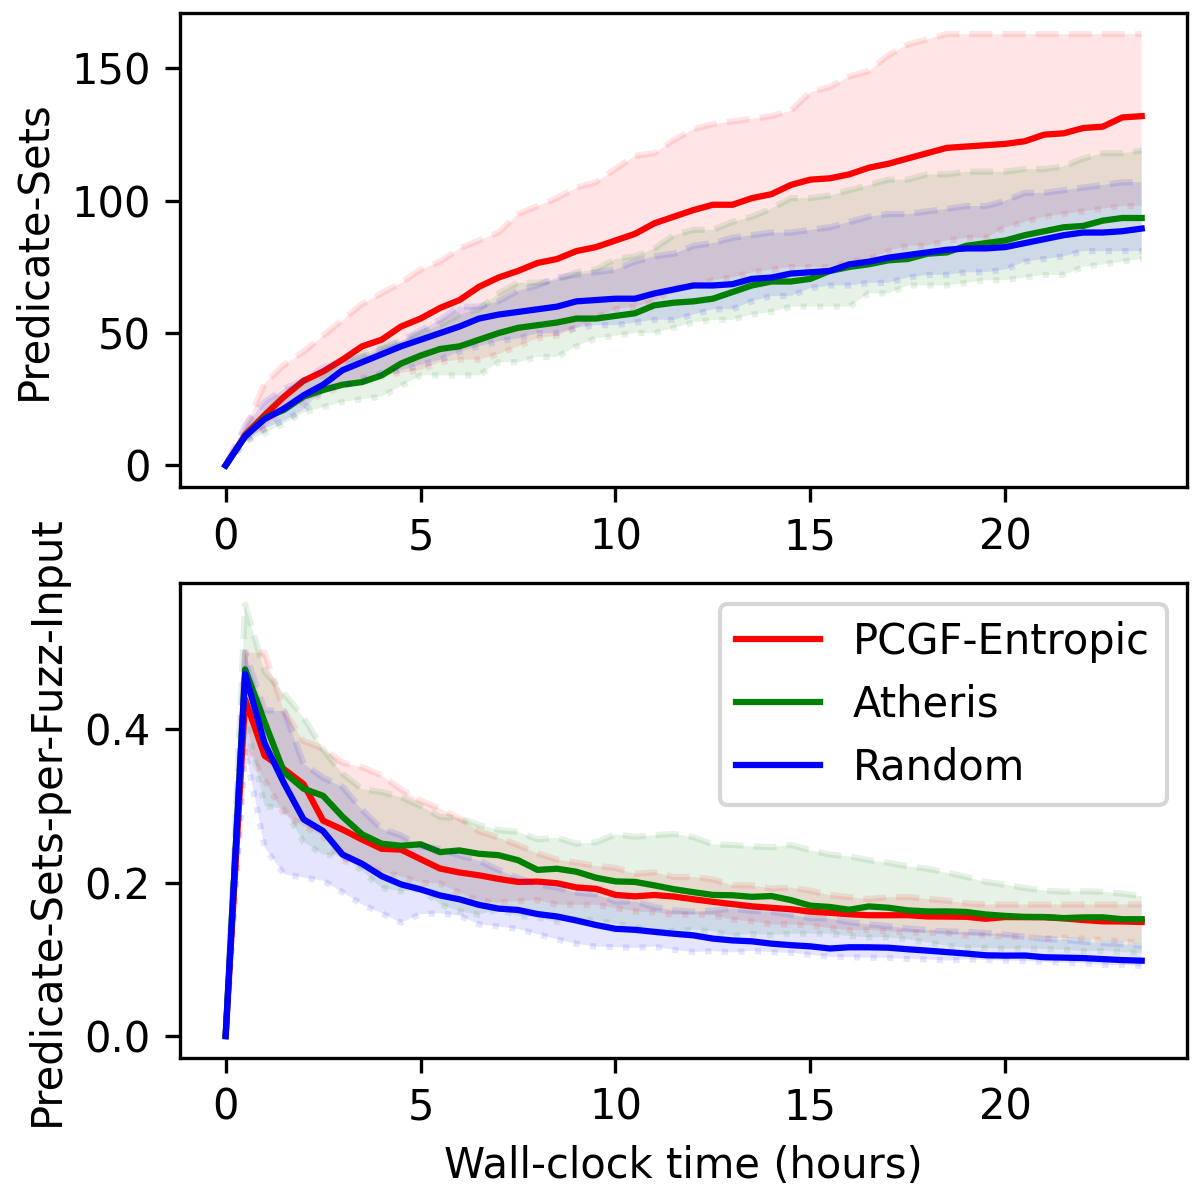
\includegraphics[width=0.6\linewidth]{figures/chapter5/RQ1/(PCGF-Entropic,Atheris,Random)_TFPP_all-coverage_(Predicate-Sets,Predicate-Sets-per-Fuzz-Input).png}
    \caption{RQ1, TF++ agent.}
    \label{fig:RQ1-TFPP}
\end{figure}

\begin{figure}
    \centering
    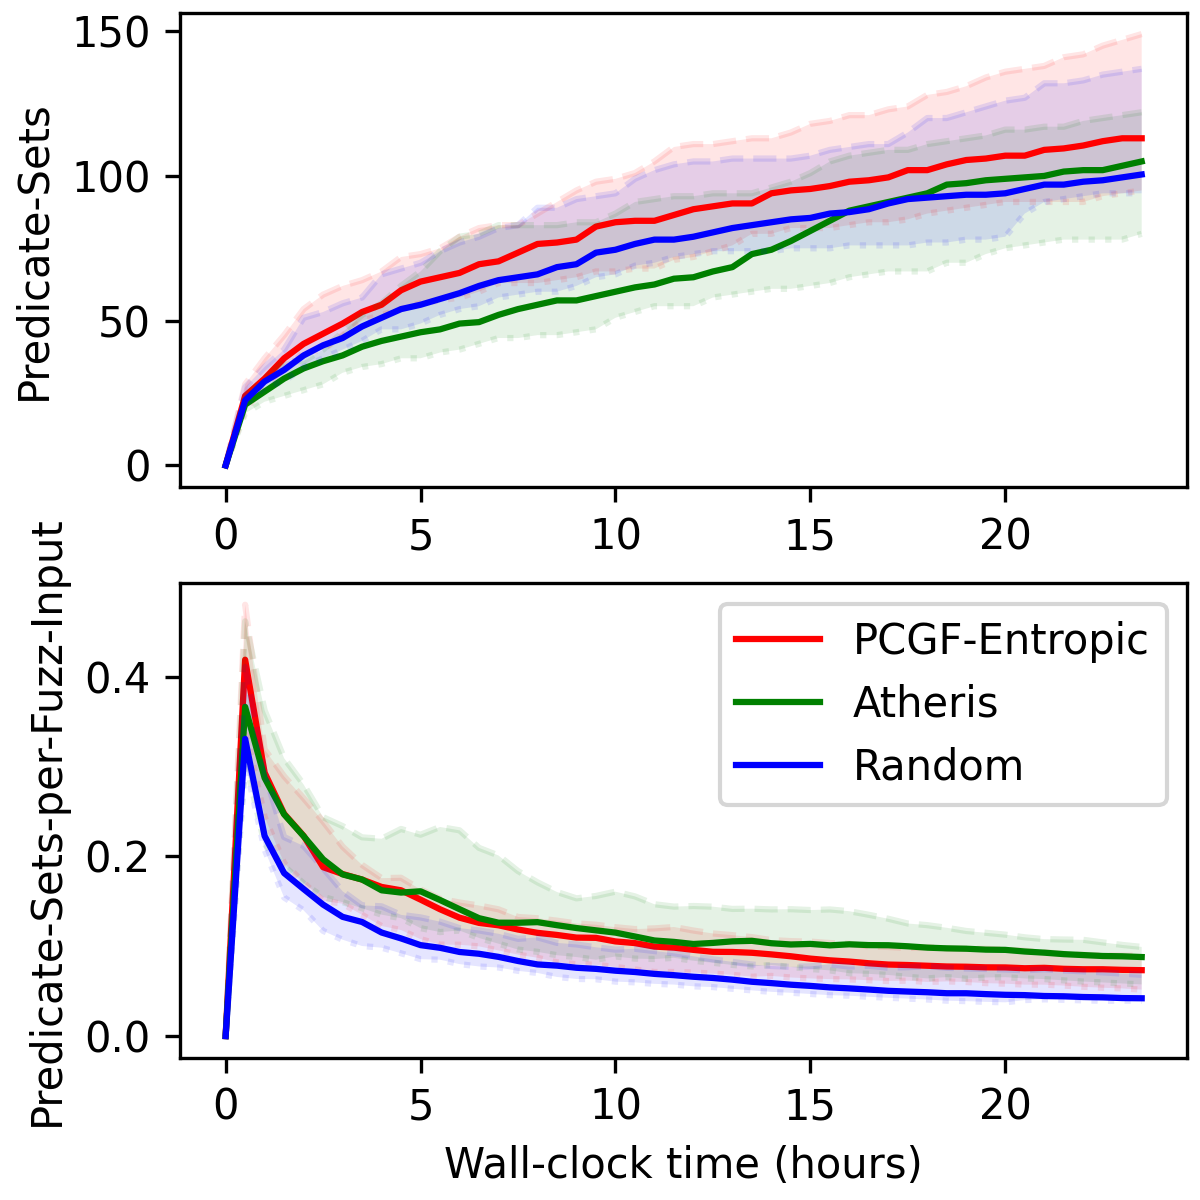
\includegraphics[width=0.6\linewidth]{figures/chapter5/RQ1/(PCGF-Entropic,Atheris,Random)_autopilot_all-coverage_(Predicate-Sets,Predicate-Sets-per-Fuzz-Input).png}
    \caption{RQ1, CARLA autopilot agent.}
    \label{fig:RQ1-autopilot}
\end{figure}

\begin{figure}
    \centering
    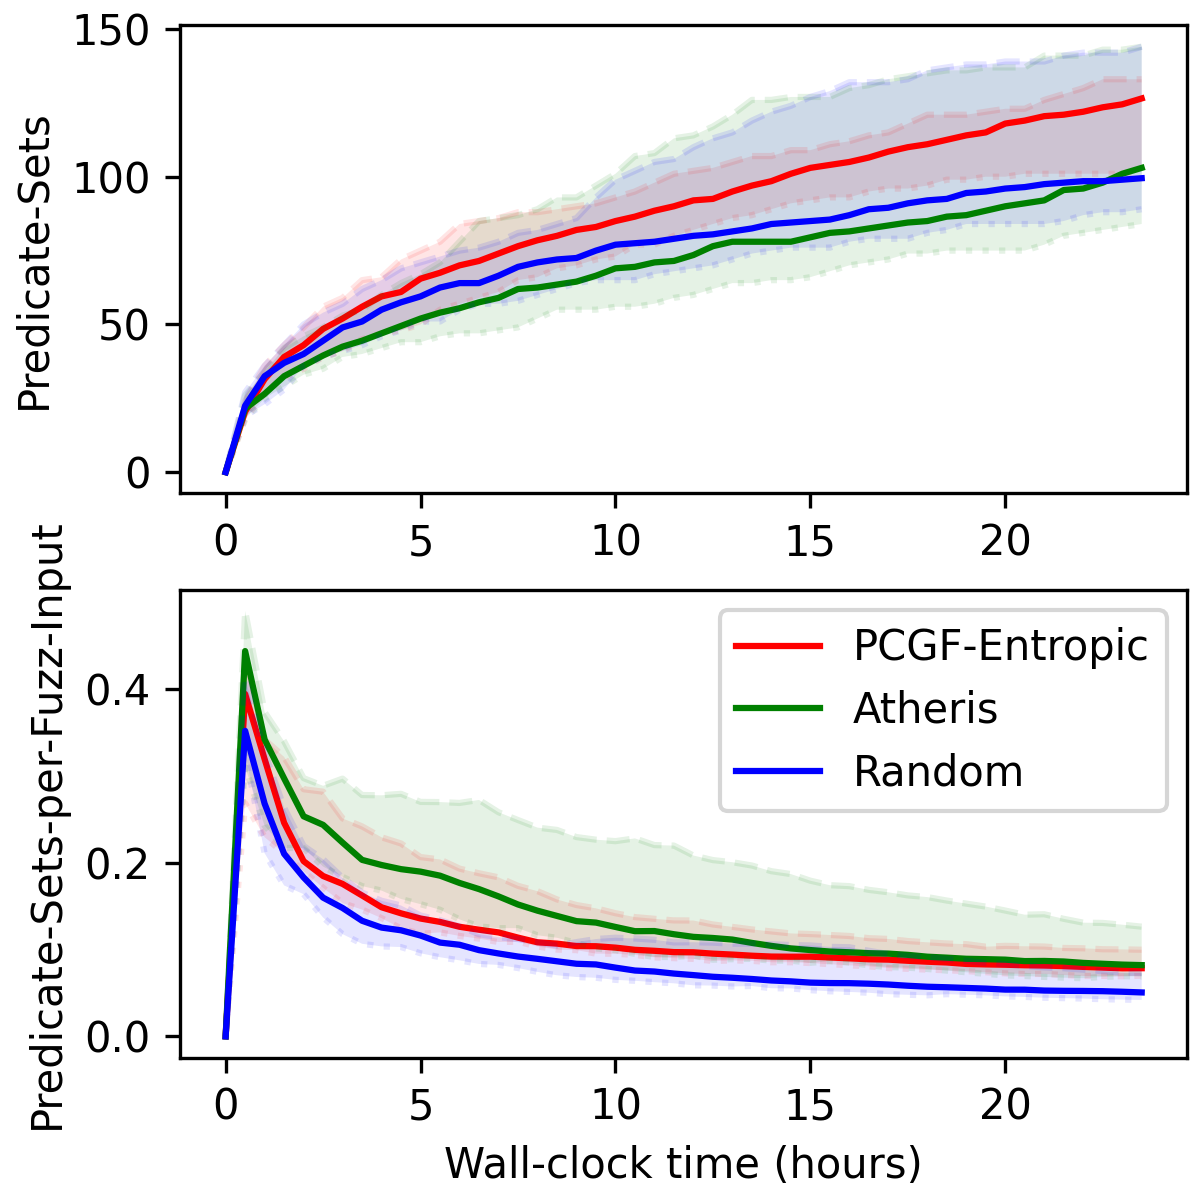
\includegraphics[width=0.6\linewidth]{figures/chapter5/RQ1/(PCGF-Entropic,Atheris,Random)_BehaviorAgent_all-coverage_(Predicate-Sets,Predicate-Sets-per-Fuzz-Input).png}
    \caption{RQ1, CARLA BehaviorAgent agent.}
    \label{fig:RQ1-BehaviorAgent}
\end{figure}

\begin{figure}
    \centering
    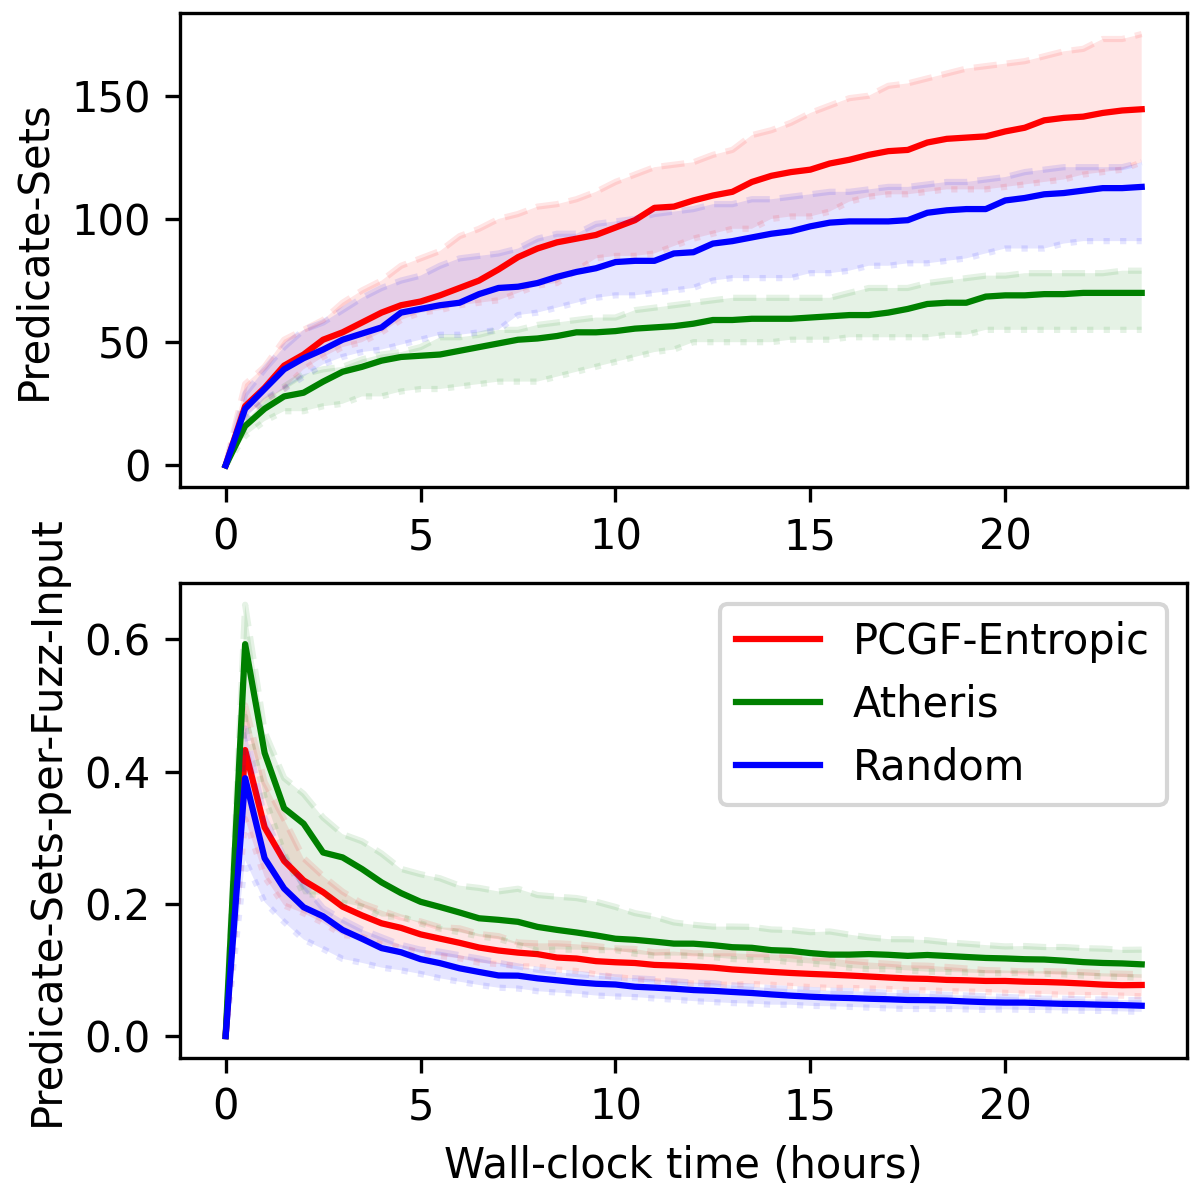
\includegraphics[width=0.6\linewidth]{figures/chapter5/RQ1/(PCGF-Entropic,Atheris,Random)_intersectionAgent_all-coverage_(Predicate-Sets,Predicate-Sets-per-Fuzz-Input).png}
    \caption{RQ1, SCENIC agent.}
    \label{fig:RQ1-SCENIC}
\end{figure}




%---------------------
\subsubsection{Results}

Our coverage criterion is to increase the cumulative number of unique predicate evaluations.
% 
Furthermore, it is desirable to achieve this coverage in as few test scenarios as possible.
% 
The evolution of coverage metrics over time and the coverage improvement per valid fuzz input for all the techniques for each agent are provided in Figures~\ref{fig:RQ1-TFPP},\ref{fig:RQ1-autopilot},\ref{fig:RQ1-BehaviorAgent},\ref{fig:RQ1-SCENIC}.
% 
In each figure, the different techniques are color coded; the solid curve shows the median coverage of all the trials and the bank around it shows the range, i.e., the minimum and maximum coverage obtained by each trial.
% 
The minimum coverage trial is dotted, and the maximum coverage trial is dashed.




We would like to highlight a few important aspects of the results.
% 
First is that the predicate coverage guided fuzzer that implements the Entropic power schedule (PCGF-Entropic) outperforms both the random fuzzer and Atheris irrespective of the AV agent under test.
% 
This observation is not surprising since a custom fuzzer to improve a specific metric is expected to improve the metric.
% 
However, we emphasize that the coverage obtained by PCGF is better than random and Atheris for any amount of computation budget allocated to it for a wide variety of AV agents.


Second, while random fuzzer achieves the same coverage as Atheris for most agents, it generates a lot more test-case instances.
% 
This is because the computational resources required to generate a new input using randomization is very low, as a result, it generates several test instances.
%
This difference gets amplified in the case of the SCENIC agent since SCENIC's NewtonianSimulator does not need heavy computational resources e.g. for rendering graphics.
% 
Therefore, if one considers the coverage-per-fuzz-input metric, random fuzzer always performs worse than the other two.


\begin{table}[]
    \centering
\begin{tabular}{|c|c|c|c|}
\hline
 & Random & Atheris & PCGF-Entropic\\
\hline
TF++ & 92, 920 & 97, 670 & 132, 929 \\
BehaviorAgent & 108, 2088 & 104, 1241 & 124, 1553 \\
AutoPilot & 107, 2400 & 104, 1298 & 118, 1692 \\
Scenic agent & 112, 2589 & 70, 668 & 150, 2009 \\
% Old numbers with violations.
% TF++ & 92, 920, 8 & 97, 670, 7 & 132, 929, 8\\
% BehaviorAgent & 108, 2088, 12 & 104, 1241, 12 & 124, 1553, 14\\
% AutoPilot & 107, 2400, 7 & 104, 1298, 8 & 118, 1692, 8\\
% Scenic agent & 112, 2589, 4 & 70, 668, 3 & 150, 2009,5\\
\hline
\end{tabular}
    \caption{Table documenting the performance of different fuzzing techniques on different AV agents. Each cell contains the median coverage obtained by the techniques and the total number of valid fuzz inputs generated.}
    \label{tab:all-medians}
\end{table}

Table~\ref{tab:all-medians} summarizes the median coverage and the median number of valid fuzz inputs generated for a given fuzzing technique on a given agent.
% 
% We calculate the unique set of predicates covered as the predicates that are covered by this technique but were not covered by the other two.
% 
From Table~\ref{tab:all-medians}, it is clear that PCGF-Entropic is simple enough to generate several valid fuzz inputs, but also mutates the vehicles behaviors in sufficiently complex ways to improve coverage.
% 
While Table~\ref{tab:all-medians} quantifies the benefits of using predicate coverage guided fuzzer, the temporal evolution of the number of fuzz inputs highlights that for any computation budget, the coverage-guided fuzzer returns a better coverage.
 


\subsection{RQ2: What type of Fuzzing Algorithm is better for generating a Diverse test suite?}


One of the biggest advantages of fuzzing is that it can be customized to any domain with custom fuzzers, power schedules, and custom coverage or goal criterion.
% 
In RQ1, we observed that predicate coverage feedback outperforms code coverage feedback (Atheris) and no feedback (random fuzzing).
% 
In this section, we investigate whether changing the feedback or the power schedule would result in a change in coverage metric.
% 
To this end, we consider two of the most widely used power schedules in fuzzing, namely AFLFast and Entropic. 
% 
In contrast to AFLFast, Entropic can be provided with multiple coverage criterion as feedback.
% 
Our goal is to discover the most suitable power schedule and the feedback to improve the scenario coverage. 
%
We continue the experimental set up of RQ1, i.e., the same coverage metrics, mutators, seeds, and AV agents, and modify the power schedules and the feedback.


\subsubsection{Fuzzers}
\begin{itemize}
    \item PCGF-AFLFast.
    We implemented the AFLFast power schedule \cite{fuzzingbook2023:GreyboxFuzzer} and used it together with using predicate-sets for the fuzzing feedback.

    \item PCGF-Entropic.
    This is the fuzzer that we used for RQ1.

    \item PCGF-Entropic-MixedFeedback
    The Entropic power schedule allows having a fuzzing feedback that is comprised of several features of different types\footnote{These feature types are called \emph{species} in the Entropic paper.}.
    %
    Since our goal is to increase the total number of unique predicate valuations, in addition to the set of predicates, we also give the individual predicates as fuzzing feedback.

\end{itemize}



\begin{figure}
    \centering
    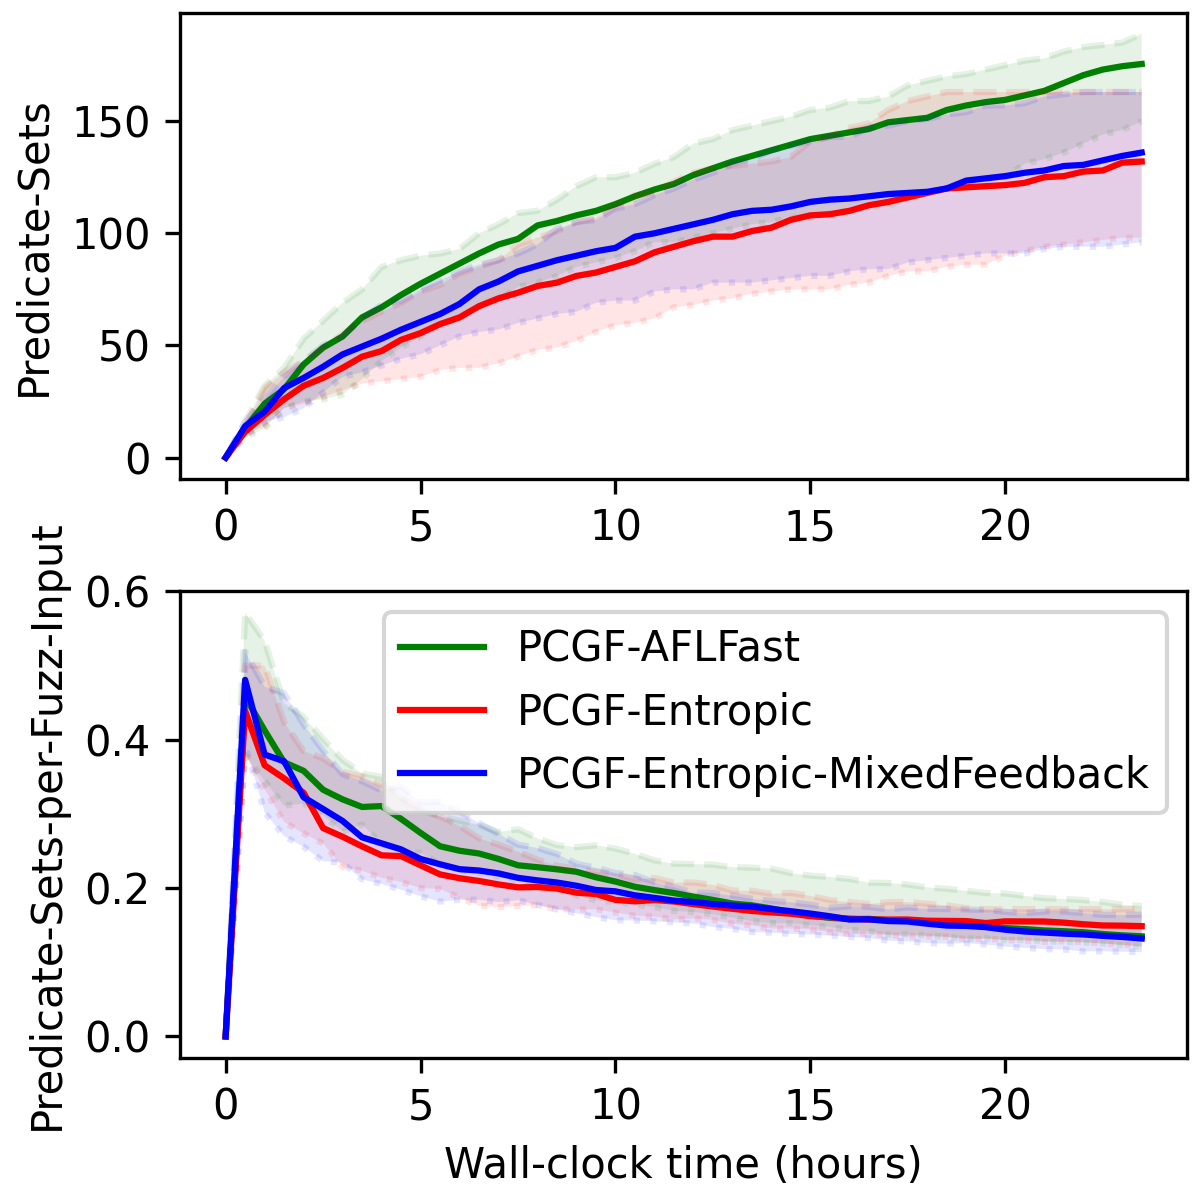
\includegraphics[width=0.6\linewidth]{figures/chapter5/RQ2/(PCGF-AFLFast,PCGF-Entropic,PCGF-Entropic-MixedFeedback)_TFPP_all-coverage_(Predicate-Sets,Predicate-Sets-per-Fuzz-Input).png}
    \caption{RQ2, TF++ agent.}
    \label{fig:RQ2-TFPP}
\end{figure}


\begin{figure}
    \centering
    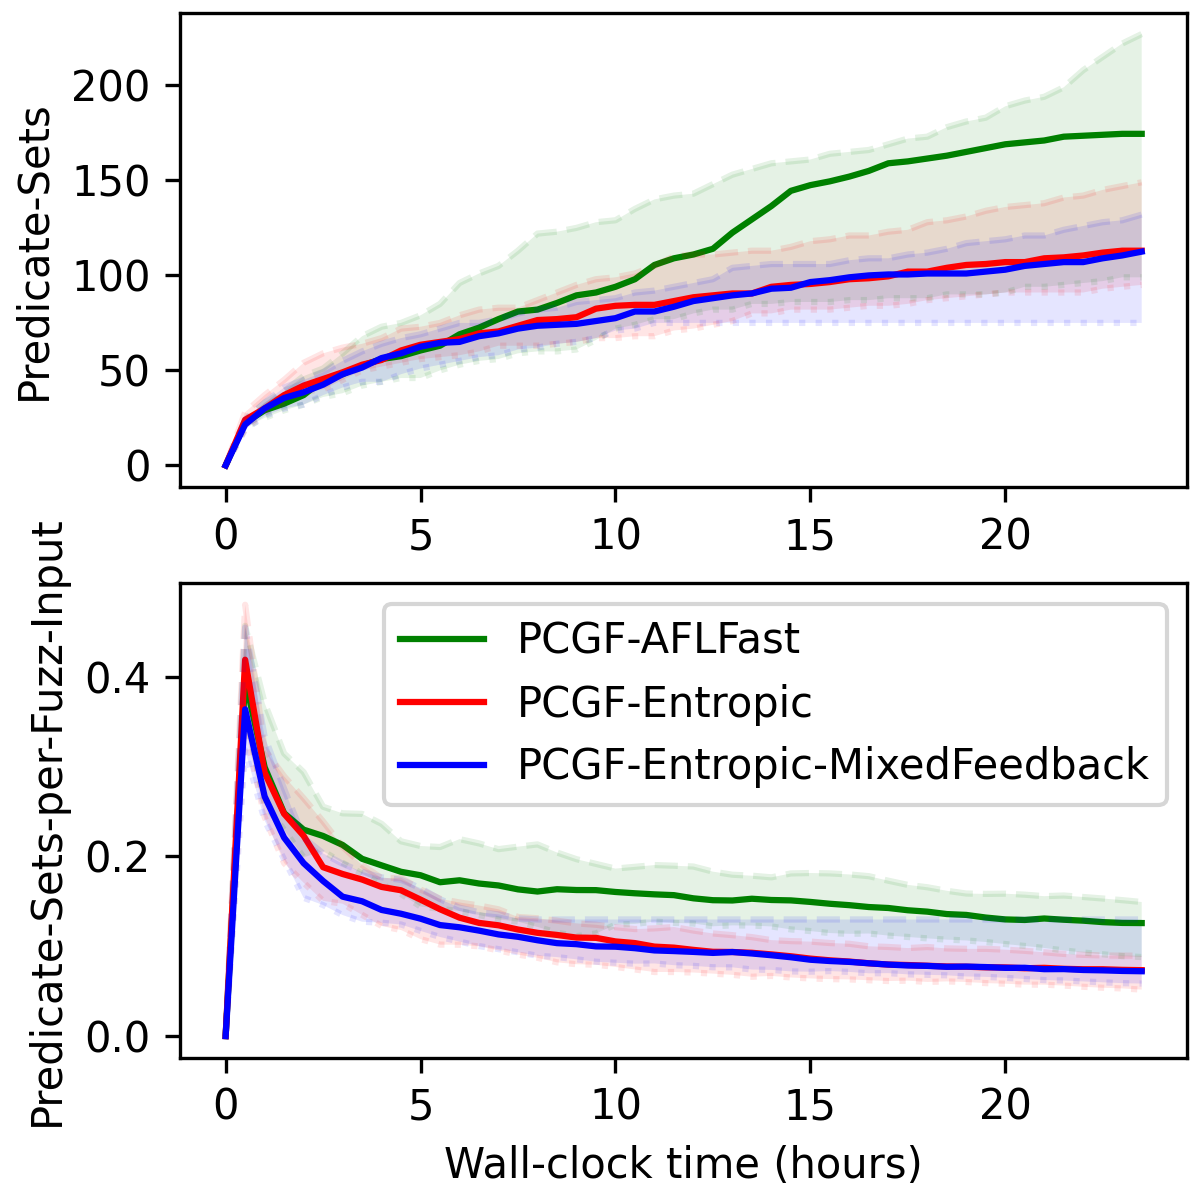
\includegraphics[width=0.6\linewidth]{figures/chapter5/RQ2/(PCGF-AFLFast,PCGF-Entropic,PCGF-Entropic-MixedFeedback)_autopilot_all-coverage_(Predicate-Sets,Predicate-Sets-per-Fuzz-Input).png}
    \caption{RQ2, CARLA Autopilot agent.}
    \label{fig:RQ2-autopilot}
\end{figure}


\begin{figure}
    \centering
    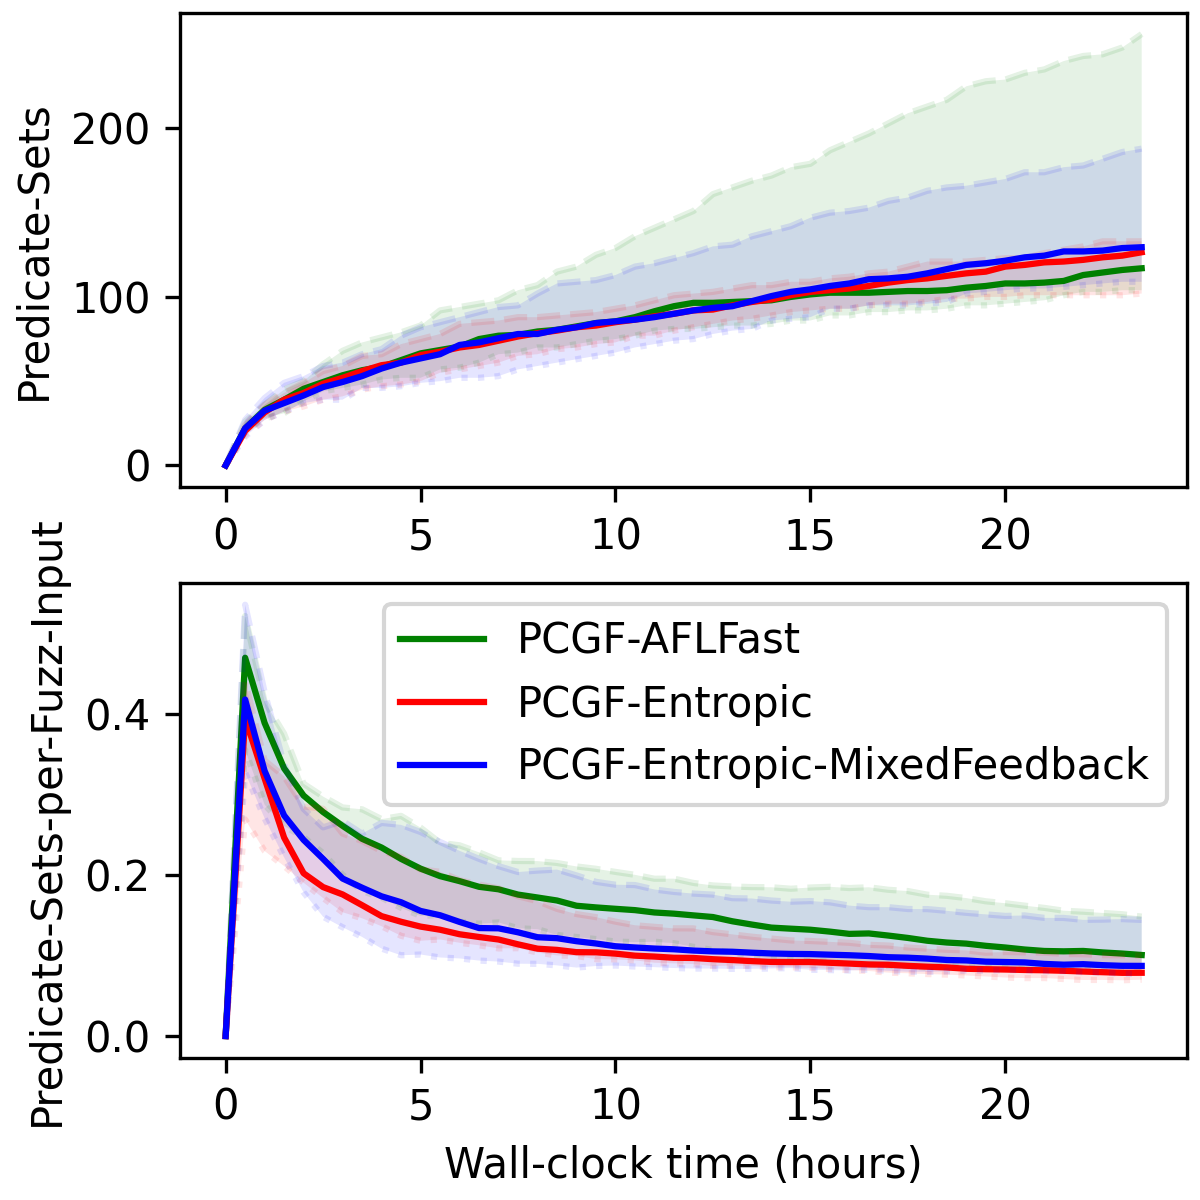
\includegraphics[width=0.6\linewidth]{figures/chapter5/RQ2/(PCGF-AFLFast,PCGF-Entropic,PCGF-Entropic-MixedFeedback)_BehaviorAgent_all-coverage_(Predicate-Sets,Predicate-Sets-per-Fuzz-Input).png}
    \caption{RQ2, CARLA BehaviorAgent agent.}
    \label{fig:RQ2-BehaviorAgent}
\end{figure}


\begin{figure}
    \centering
    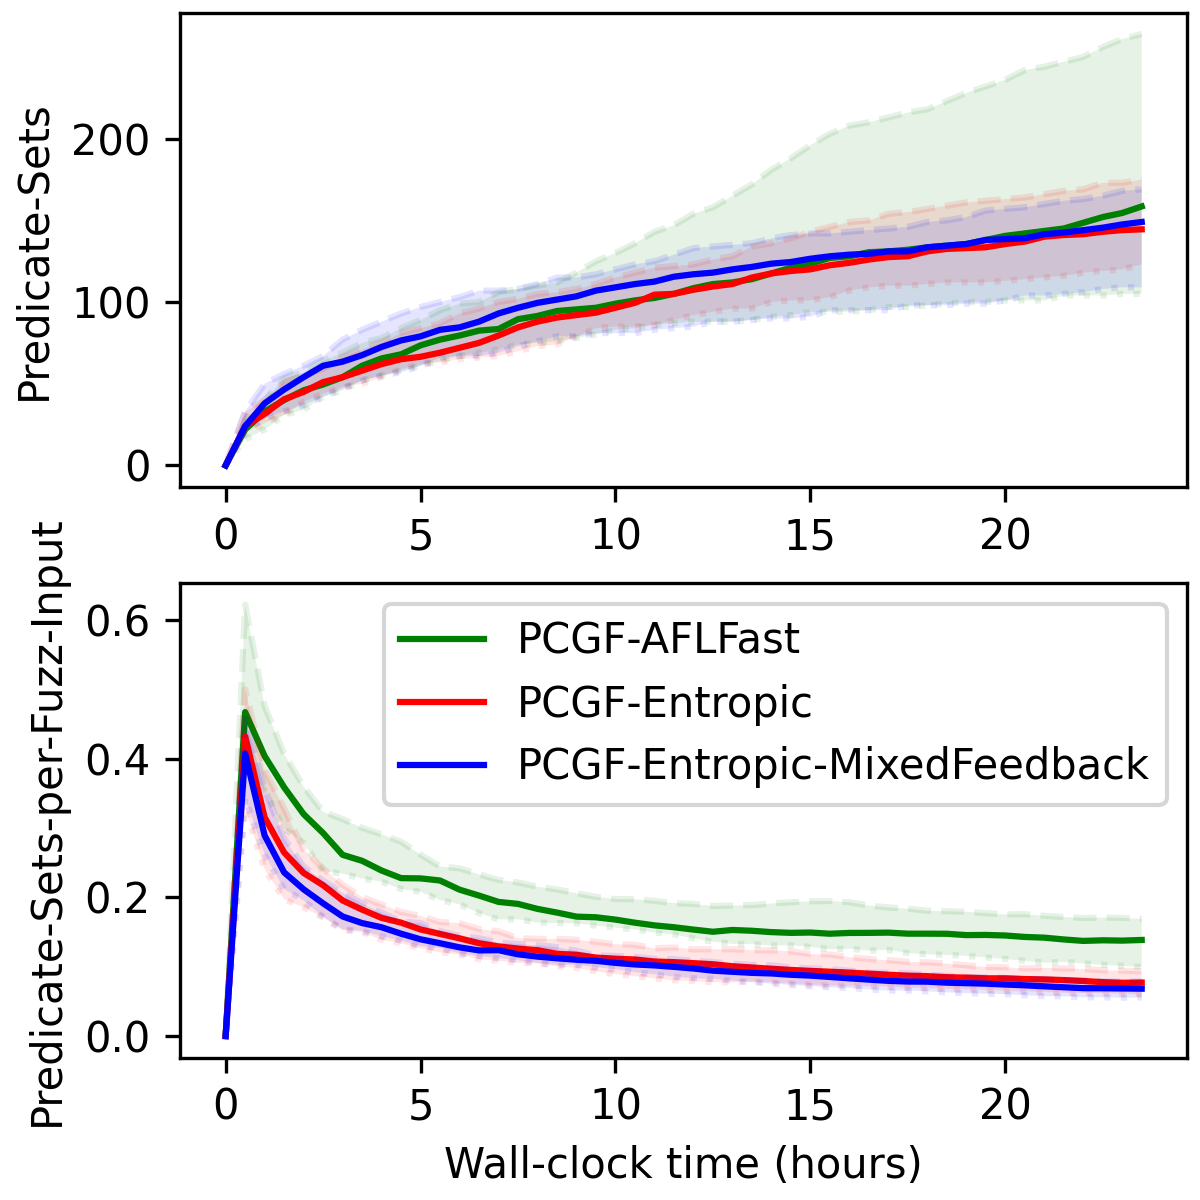
\includegraphics[width=0.6\linewidth]{figures/chapter5/RQ2/(PCGF-AFLFast,PCGF-Entropic,PCGF-Entropic-MixedFeedback)_intersectionAgent_all-coverage_(Predicate-Sets,Predicate-Sets-per-Fuzz-Input).png}
    \caption{RQ2, SCENIC agent.}
    \label{fig:RQ2-SCENICAgent}
\end{figure}


%---------------------
\subsubsection{Results}

Similar to RQ1, the evolution of coverage and coverage per fuzz input with time for all the techniques and all agents are given in Figures~\ref{fig:RQ2-TFPP},~\ref{fig:RQ2-autopilot},~\ref{fig:RQ2-BehaviorAgent},~\ref{fig:RQ2-SCENICAgent}.
% 
We draw two conclusions from these figures: 1) AFLFast achieves better coverage for all agents than both the version of Entropic and 2) Supplementing the predicate sets with the individual predicates as feedback does not result in any significant improvement for Entropic.
% 
% Our primary observation is that AFLFast achieves better coverage for all agents than both versions of Entropic.
% 
% Our secondary observation is that supplementing Entropic with additional coverage information does not improve the coverage performace.
%


The difference between AFLFast and other fuzzers is more pronounced in TF++ and Autopilot.
%
Also notice that the reason for AFLFast achieving better coverage is not because it generates more test cases.
% 
AFLFast outperforms other fuzzers in the coverage-per-fuzz-input metric too.
% 
The advantage of AFLFast over Entropic is contrary to our intuition as we expected the simplicity of AFLFast to come with a price.
%
The authors could not think of a reason for this clear improvement in performance of AFLFast; we would be glad if informed reviewers who are domain experts in fuzzing can help us in this regard.


The authors did not anticipate such a difference in coverage as a result of changing the power schedule.
% 
This surprising result might indicate that our platform can be a good candidate for benchmarking different fuzzing algorithms.
% 
% Furthermore, our experiments might provide a good benchmark for comparing fuzzing algorithms.



\subsection{RQ3: Do the coverage metrics transfer between AV implementation?}

In this paper, we presented a framework for improving the predicate coverage for test scenarios for AVs.
% 
One of the drawbacks of our proposed method is that it requires the AV to be deployed in-the-loop.
% 
Since different AV implementations react to the same scenario in different ways, the coverage metrics for the same collection of test scenarios can vary based on the AV implementation.
% 
This begs the question, do test cases that improve coverage for one AV implementation also work for other implementations?
% 
Such transfer of coverage would be immensely helpful as it points out to the common set of use-cases or corner cases among different implementations.

To answer this question, we investigate the transfer of coverage metrics from one implementation to the other.
% 
That is, we collect all the test scenarios generated by the fuzzer of choice for a given AV implementation.
% 
We then subject other AV implementations to the same set of test scenarios and measure the coverage.
% 
We normalize the coverage of the current AV implementation as $100\%$ and plot the predicate coverage of the transferred AV implementation as a percentage.
% 
For example, we collect all the test scenarios generated by Atheris on CARLA Autopilot and deploy the same scenarios on CARLA BehaviorAgent, TF++, and SCENIC agent.
% 
We plot the coverage of each of the three individual agents relative to the original coverage.
% 
We use only two fuzzing methods, first is the code coverage based Atheris and second is the PCGF-AFLFast fuzzer. 
%
We perform 10 trials using $\{ 0, \dots, 9 \}$ PRNG seeds as in RQ1-2 where each trial consists of generating a corpus using a fuzzer and an ego agent, then testing the corpus on a different ego agent.
%
The PRNG seed is fixed between the generation and test experiments.
%
% For each pair different agents, we consider 10 trials using the 

% In this part, we evaluate whether fuzzing can generate high-coverage driving scenarios irrespective of AV implementation.
% 


%---------------------
% \subsubsection{Performance Metric}
% Ratio of coverage sizes, where the target coverage is when the original ego agent is used to generate the test-cases, and the test coverage is when the different test ego agents are tested on the test-suite
% 
% 
% \subsubsection{Fuzzer}
% We use PCGF-AFLFast for this part, since it was the best performing fuzzer, also that the experiments for the other fuzzers did not finish in time for the submission deadline.


%---------------------
% \subsubsection{Trials}


\begin{figure}
    \centering
    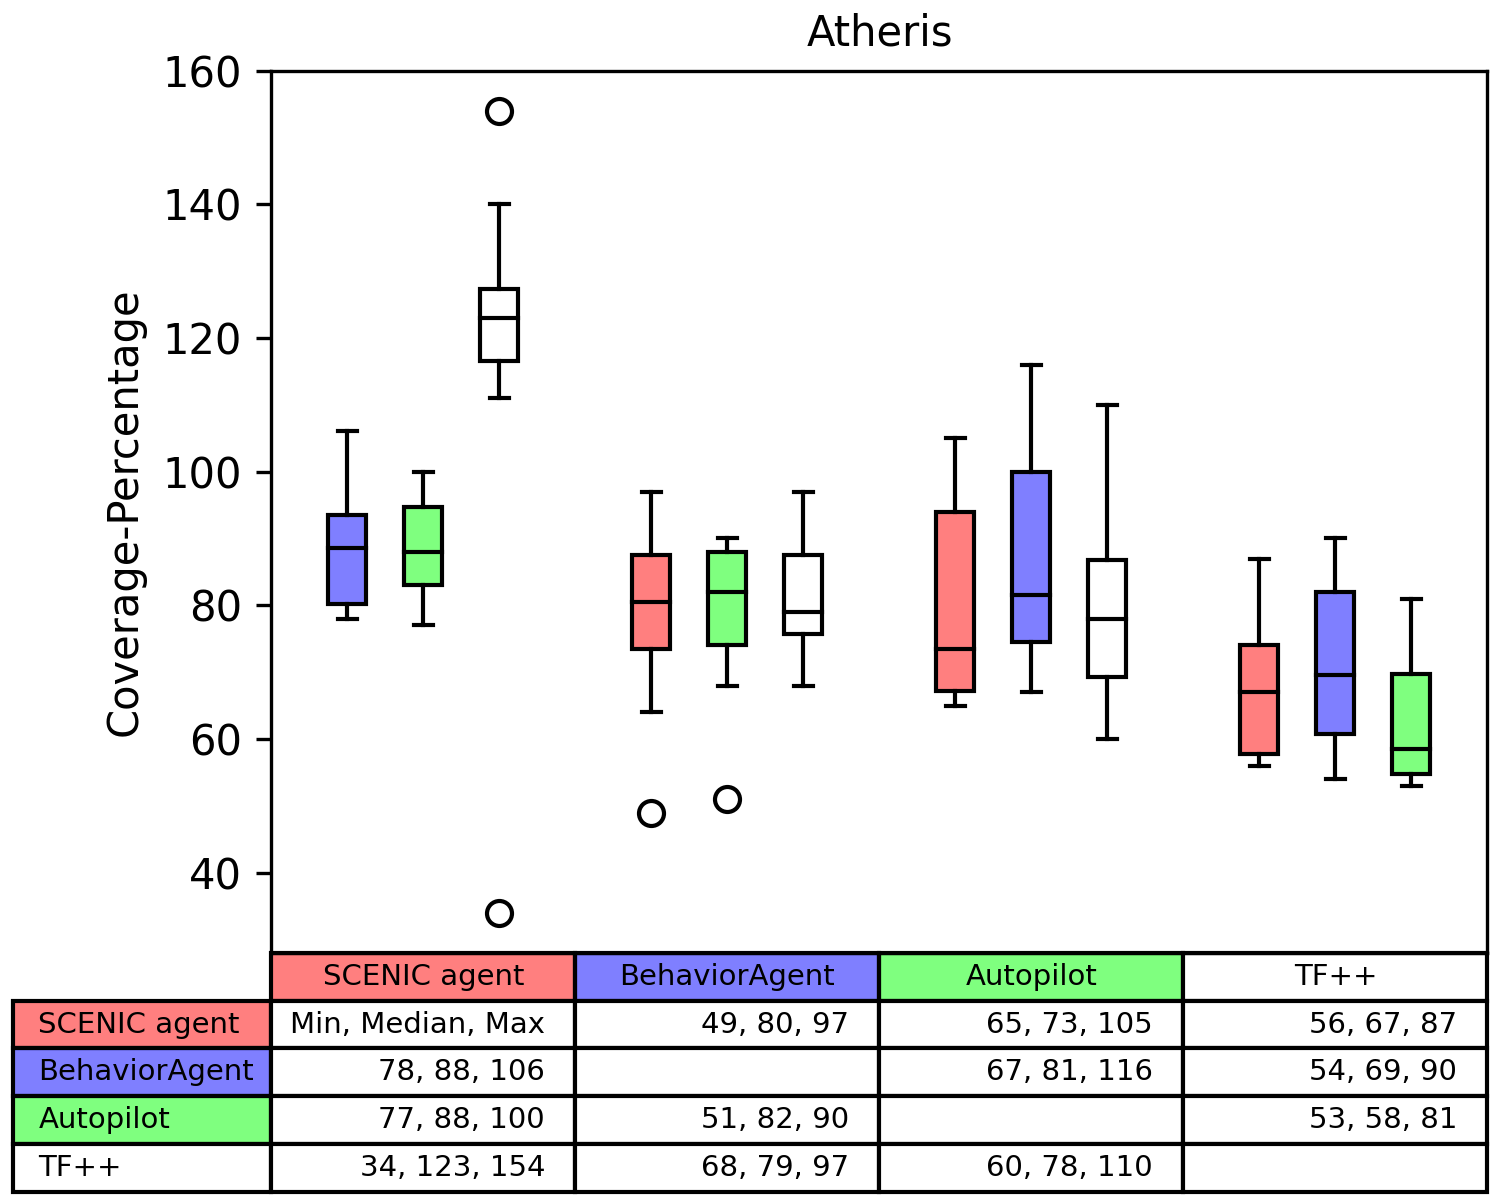
\includegraphics[width=0.7\linewidth]{figures/chapter5/RQ3/Atheris_traffic-rules_all-coverage_PredicateSetCoverage_Coverage-Percentage.png}
    \caption{Common set of scenarios for different agents}
    \label{fig:switch-agent_Atheris}
\end{figure}

\begin{figure}
    \centering
    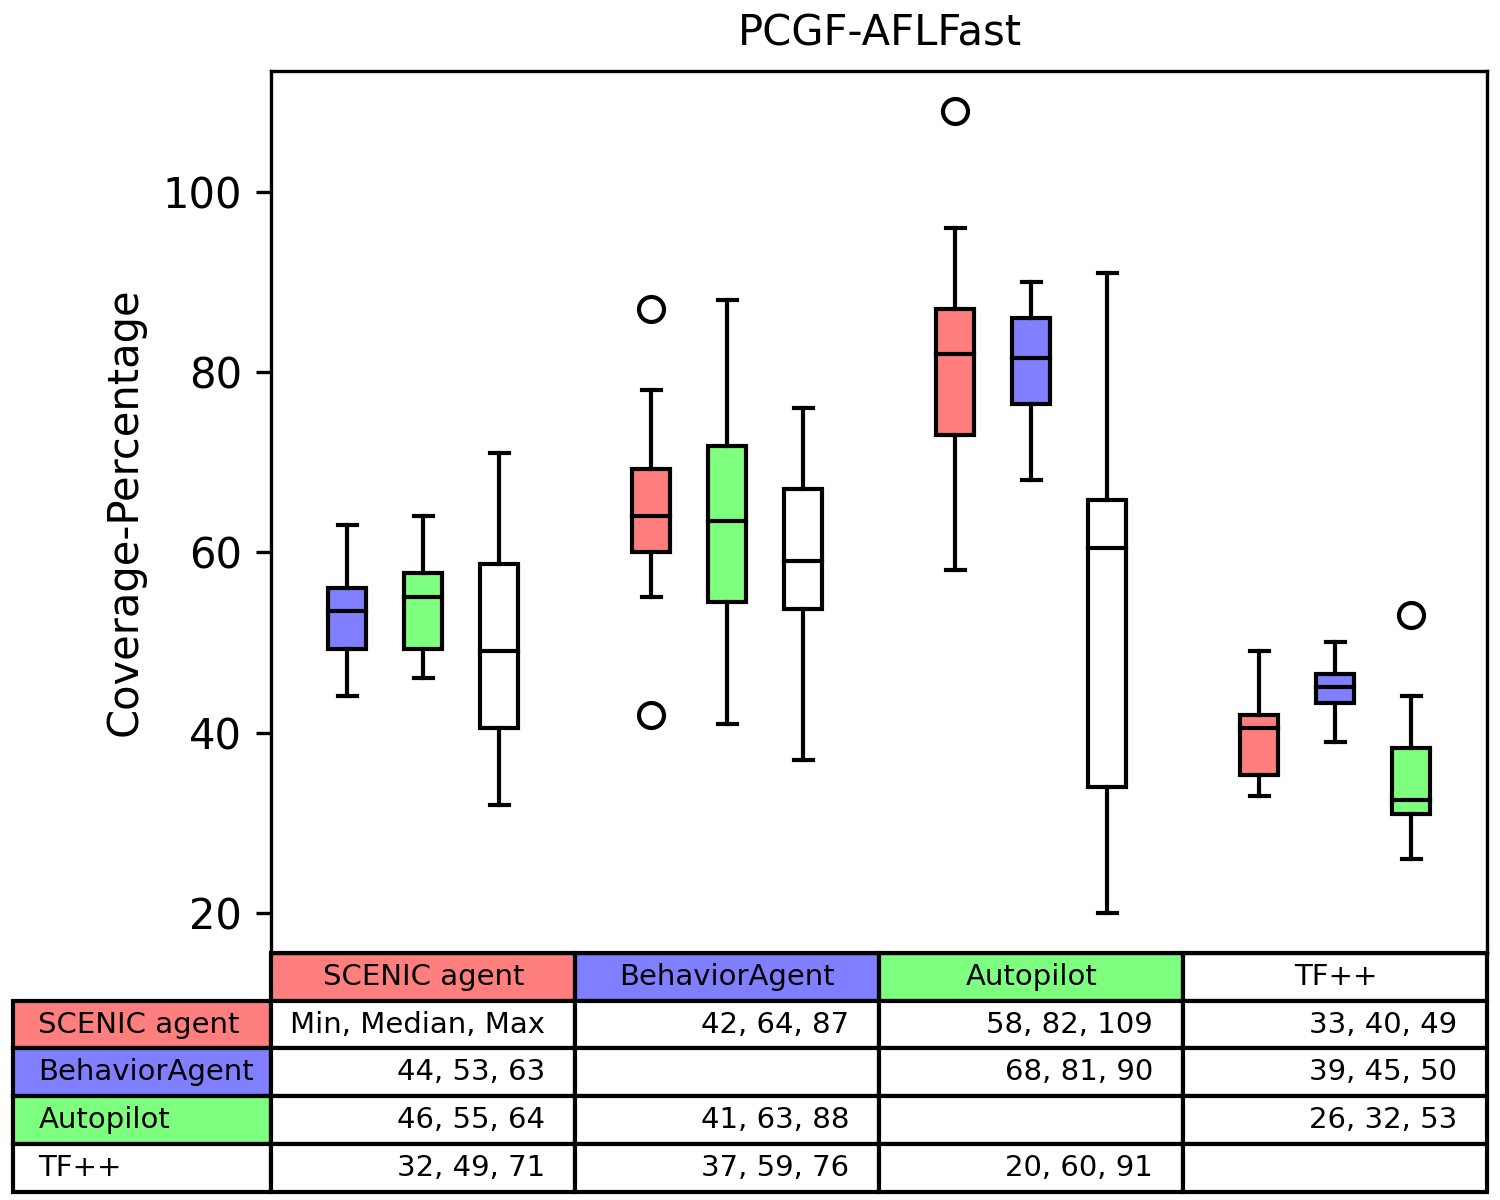
\includegraphics[width=0.7\linewidth]{figures/chapter5/RQ3/PCGF_traffic-rules_all-coverage_PredicateSetCoverage_Coverage-Percentage.png}
    \caption{Common set of scenarios for different agents}
    \label{fig:switch-agent_Random}
\end{figure}

%---------------------
\subsubsection{Results}
The transfer of coverage metrics from one AV implementation to another are presented in Figure~\ref{fig:switch-agent_Atheris} and Figure~\ref{fig:switch-agent_Random}.
% 
Each column of the table shows the agent used to generate the corpus, and each row shows the agent tested on the resulting corpus.
%
The entries of the table show the minimum, median, and maximum of the metric accross the 10 trials.
%
Above the table, we show the standard box-plot of the results, i.e. quartiles, median, and fliers.


The first observation is that scenarios generated for one agent are indeed reusable for other agents.
%
For code driven fuzzing tool Atheris, on average, one can obtain $70\%$ of the original coverage by applying the same set of test cases to a different implementation; this number drops close to $50\%$ for PCGF-AFLFast.
% 
% \textbf{Insert a line here for PCGF-AFLFast and compare if it is higher or lesser}.
%
% 
% 
Another observation is that transfer of coverage is better between Autopilot, SCENIC agent, and BehaviorAgent as opposed to TF++.
% 
One possible reason is that all these three agents do not implement perception processing and the maps and relative positions of other vehicles is provided to these agents by the CARLA environment.
% 
This also explains why the coverage metrics from TF++ transferred poorly to other agents because TF++ learns the road network and the position of other agents through perception.
% 
The authors would like to confirm this hypothesis by conducting more experiments on open source end-to-end CARLA Leaderboard agents; however, much to our chagrin, we couldn't find one.
% 

The second observation is that the scenarios generated using PCFG-AFLFast transfer poorly when compared to Atheris for almost all instances.
% 
This highlights that while PCGF-AFLFast increases scenario coverage, it improves the coverage for a specific AV implementation.
% 
From the results of RQ1, we remarked that PCGF is fast enough to generate more number of test scenarios and accurate enough to improve coverage; however, this evaluation highlights that the coverage is implementation specific.

The third observation is that in some instances the predicate coverage transfer is more than $100\%$. 
% 
While this may be counterintuitive, it deserves some explanation.
% 
Consider a test-suite $\{ s_1, s_2 \}$ for a given AV implementation, say CARLA Autopilot.
% 
If we subject a different AV implementation, say TF++, to these two scenarios $s_1$ and $s_2$, TF++ might react in different ways than Autopilot; causing an increase in the predicate coverage.




\section{Threats to Validity}

\textbf{Internal Validity:} Internal validity threats concern factors in the
experiments that may affect the results.
% 
We have chosen an appropriate baseline (random generation) and have repeated the experiments for 10 times (each run for 24 hours) and plotted the median of the random runs.
% 
Furthermore, none of the AV agents tested were developed in-house, but all the agents are publicly available.

\textbf{External Validity:} The primary threat to external validity of our technique is the applicability of the results in a physical deployment.
% 
Since all the experiments are conducted in a simulation environment, the vehicle parameters such as velocity profiles and trajectories might not be practical.
% 
This would be an issue with any simulation based test-case generation for AVs.
% 
To mitigate this, we have made our evaluation platform to be able to test any AV agent compatible with CARLA Leaderboard 2.0.
% 
Our extensive experimentation to include 4 different publicly available agents and assessing the mutual coverage of the test results is to ensure that the proposed techniques works for as many agents as possible.
%
Furthermore, our evaluation looks at AVs with different information available to them --- from TF++ where the AV agent infers the road network and the behavior of other AVs from sensors --- to CALRA Autopilot that has map and other agent information provided to it from the simulation engine. 
% 
However, since we do not evaluate our technique on any \emph{real} AV implementation, this threat remains unresolved.

\textbf{Construct Validity:} In this paper we propose a new notion of coverage --- predicate coverage --- where the predicates model aspects of the AV behaviors required for inferring AV's compliance with traffic rules.
% 
Given that we also propose a new predicate guided fuzzing technique that improves the predicate coverage, we acknowledge the circularity in the argument.
% 
However, such circularity would be a part of any coverage guided fuzzing technique --- the fuzzing technique customized to improve the coverage of a given metric, indeed improves the coverage of the metric.
% 
We believe that since the predicates of AV are predicates on the behavior of AV and not just the code of software, the increase in coverage does lead to new behaviors.
% 


% and highlight that purely using code coverage techniques do not outperform random scenario generation.
% % 
% Since the predicates of interest are a function of physical AV behaviors, 

% \begin{itemize}
%     \item External Validity. All these are generated in simulation environment. Validity for real platforms is still unclear. To mitigate this, 4 different types of agents. Further, our system can work with any AV agent that can work with CARLA leaderboard 2.0
%     \item Construct Validity. Circularity --- new metric and fuzzing that optimizes for this metric is better.
% \end{itemize}


% \begin{itemize}
%     \item I have seen people just do fluff.
%     \item Add two paras as to what are some challenges.
% \end{itemize}
\section{Related Work}
There are several papers in the literature that focus on generating test scenarios for autonomous vehicles.
% 
These can be divided into two main classes.
% 
The first class includes papers that use mathematical logic and formal semantics for generating test scenarios.
% 
The second class includes papers that target a specific type of system failure such as a safety violation such as a collision or violation of a prescribed traffic behavior.
% 
% Make different sections and address related work in different sections.

\subsection{Scenario Generation Using Formal Semantics}
SCENIC is one of the first tools to present a probabilistic programming language for automatically generating test scenarios for autonomous vehicles~\cite{fremont2019scenic}.
% 
Given a high-level description of the configurations of the vehicles and the road network in a probabilistic programming language, SCENIC generates various scenes from the distribution described by the program.
% 
In contrast to SCENIC, the current work does not generate test scenarios according to a distribution, but rather to improve the predicate coverage of AVs.
% 
Some related works capture some functional aspects of AV behaviors such as adherence to traffic rules~\cite{maierhofer2020formalization} and safety violations~\cite{dreossi2019verifai} as statements in signal temporal logic~\cite{tuncali2016utilizing}.
% 
These works then use either fuzzing or falsification techniques for generating various test cases.
% 
Unlike these works, our goal is not to find just behaviors that violate the functional or safety specifications, but rather to explore a variety of ways in which an AV can violate the requirements e.g. traffic rules.
% 
Using formal semantics of traffic rules in custom logic~\cite{Karimi.2020, Bozga.2022} and generating test cases using these have been proposed in~\cite{karimi2022automatic,li2023simulation}.
% 
While the test scenarios generated in these works do increase coverage, these works are not explicitly driven to increase the coverage of AV behaviors.

\subsection{Goal Driven Test Scenario Generation}
Several works in the literature have been targeted towards generating test scenarios that violate the safety properties of AVs.
% 
These are again broadly classified into two classes.
% 
The first class consists of works that modify the perception inputs~\cite{tian2018deeptest,zhang2018deeproad} for an AV and observe the effect of the perception changes on the vehicle behavior.
% 
These works have been able to show that a change in environmental conditions can drastically change the behavior of AV and in some instances violate some crucial safety specifications.
% 
Some of the works also explicitly determine the \emph{features} that are important for perception in AVs, such as modifying the LiDAR image and not the camera image, etc~\cite{abdessalem2018testing}.
% 
The second class consists of works that modify the environment of an AV, such as introducing an obstacle or a pedestrian in its path, or modifying the behavior of other vehicles in the traffic configuration~\cite{Zhong.2021,li2020av}.
% 
Unlike the current work aimed at improving the coverage of the AV behaviors, the goal of these is to discover the maximum number of failure instances for AVs in a given traffic configuration.
% 

A few works look at the high level behavioral patterns of AVs and try to generate test inputs that break such rules.
% 
For example, test scenarios for AVs were synthesized in~\cite{gambi2019generating} based on real-life accidents.
% 
Similarly, when the traffic rules are formalized in STL, the most efficient test cases that break as many rules as possible are explored in~\cite{sun2022lawbreaker}.
% 
A recent work explores the most common driving patterns for AVs and generates scenarios according to these most common patterns~\cite{tian2022generating}.
% 
Some works also use generative models such as graph networks for generating highway traffic scenarios~\cite{Bi.2019}; however, these works lack explainability and do not necessarily target a behavioral pattern of AVs.
% 
Similar search for violations while making critical maneuvers such as turning or overtake using evolutionary search was explored in~\cite{luo2021targeting}
%
The work closest to ours are~\cite{sheikhi2022coverage,hu2021coverage} which tries to improve coverage but not in terms of high level behavior predicates but the physical space that is visited by the AV.
% 
Works that try to classify failures into different classes while AVs navigate through intersections have been explored in~\cite{tang2021systematic}.
% 
Some works combine the specification driven fuzzing together with modifying the environment to discover failure cases, such as~\cite{zhou2023specification,kim2022drivefuzz}.
% 
While all these works try to classify behaviors into various classes, these works are focused on finding failure instances and these do not try to focus on generating a diverse scenarios.

\chapter[~~~~~~~~~~~~Conclusion]{Conclusion}
\label{ch:conclusion}

Despite the prevalence of companies testing their autonomous vehicles on the road, there is no consensus on end-to-end requirements for AV certification and testing.
%
This dissertation aimed to address some critical aspects of this mission, particularly focusing on the formulation of the traffic rules requirements and its compliance testing for AVs.
%
In Chapter 1, we presented our thesis as follows:
\begin{quote}
\textit{
    Autonomous vehicles are required to have interpretable behavior. Formal logic can be used to give an intuitive but precise model of the traffic rules requirement. The model can be leveraged for verification and validation, namely in test-case generation and coverage arguments.
}
\end{quote}
The key contributions of this work in support of the above thesis can be summarized as follows:

    \textbf{Formulation of Traffic Rules in Formal Logic}.
    We developed a comprehensive framework for representing traffic rules in first-order logic and answer-set programming.
    %
    This formalization allows incremental modeling of the traffic rules, which is a feature of non-monotonic reasoning.
    %
    Furthermore, it allows automated reasoning on traffic rules using off-the-shelf solvers.
    %
    We also developed an application of this framework, namely generating traffic-rules-compliant traffic in simulation.

    \textbf{Development of Complexity-Driven Test-case Generation}.  
    First, we proposed a formal definition of test-case complexity.
    %
    Our definition is objective in the sense that it does not rely on subjective assessments of what features may challenge an AV to pass a test-case.
    %
    Instead, we rely directly and only on the pass-fail criteria.
    %
    Second, we propose an algorithm to generate more-complex test-case scenarios.
    %
    Our technique can handle pass-fail criteria that regard the traffic rules and right-of-way at an intersection, in addition to goal-reach and collision avoidance.
    %
    Similar to~\cite{Karimi.2020}, we expect the traffic rules to be provided in a logic program (more precisely an Answer Set Program \cite{Lifschitz.2010}).
    %
    Our algorithm takes as input the geometry of the traffic intersection, traffic rules to be followed at the intersection, and the routes of the vehicles and generates several test-case scenarios with increasing order of complexity.
    %
    Our algorithm gives full coverage over some subspaces of the possible test-cases: after the set of lane events of two cars are fixed, there are only a finite number of relative temporal order of these events that may result in a more complex test-case, and our algorithm uses an ASP solver to do an exhaustive search over this subspace.
    %
    Third, we generate test-cases for a four-way stop, a T-intersection, and an uncontrolled Y-intersection.
    %
    Then we execute these test-cases to test CARLA's autopilot and autopilot-plus-RSS in the CARLA simulator.
    %
    We incrementally increased the complexity of test-cases and discovered instances where the CARLA autopilot failed test-cases by violating a traffic rule or colliding with a non-ego vehicle.
    %
    Also we observed that restricting the behavior of CARLA's autopilot with RSS improved its rate of success, but did not guarantee passing a test-case.

    \textbf{Comparison of techniques for Coverage-Driven Test-case Scenario Generation}.
    First, we proposed a new predicate coverage metric for AV behaviors that is explainable and can express several important aspects of their functional correctness.
    % 
    Second, we proposed coverage driven fuzzing algorithms for improving the predicate coverage of AV implementations at intersections.
    % 
    We demonstrated that fuzzing techniques that are driven by predicate coverage outperform code coverage and random fuzzing.
    % 
    Third, we investigated what type of coverage metrics and power schedules are more suitable for generating a diverse set of traffic scenarios.
    % 
    Finally, we investigated if test scenarios generated for one implementation can be used for other implementations and report our findings.
    % 
    We evaluated the algorithms in a robust manner by generating test cases for four different publicly available AV implementations on the CARLA platform.





%----------------------------------------
\section{Future Work}

This dissertation lays the foundation for several directions for future research and development:
%-----------------------------------
\subsection{Coverage-driven Fuzzing}
In this dissertation we examined the effectiveness of fuzzing for coverage-driven test-case generation and got encouraging results.
%
We propose a few more research questions in this direction.

%----------------------
\textbf{Nonego Models.}
The first question is, what nonego models are suitable for the fuzzing framework?
%
In this dissertation we used BSplines for representing trajectories, for their \emph{local control property} which allows mutation-based local search, their compact representation using the control points, and their richness which subsumes the class of kinematically/dynamically feasible trajectories.
%
An interesting alternative is representation using Behavior Trees.
%
This representation is widely used in robotics and video games since it allows modeling reactive agents, it is modular and interpretable, and allows using other models as building blocks.
%
The modularity of behavior trees is helpful for fuzzing as it allows structure-aware mutation operators.
%
Another curious alternative is data-driven models, e.g. generative models in machine learning.
%
Having such models, we can investigate the question of whether fuzzing the generative model would help with predicate coverage, compared to the baseline of randomly sampling from the generative model.
%
On possible challenge here is that the scenario encodings in generative models are usually unstructured, represented simply as a vector of numbers, which prohibits using structure-aware mutation.

%-----------------------------------------
\textbf{Transfer of Coverage between AVs.}
In this dissertation we observed an asymmetric transfer of coverage between the rule-based agents and the learning-based agent.
%
This encourages further investigations, which would require integrating more machine-learning-based AV agents into our CARLA platform.
%
Another interesting question is, whether the transfer of coverage depends on the nonego models (BSplines, behavior trees, etc.)



%-----------------------------------
\subsection{Complexity-driven Testing}
In this dissertation we proposed a formal notion of complexity, capturing the difficulty level of passing a test-case.
%
We believe that the formal definition is powerful in the sense that it directly captures the informal notion of test-case difficulty level.
%
However, this generality comes with the representation and computation challenges.
%
In our work, we studied some special cases where we can compute the complexity partial order exactly.
% 
However, in many applications we rather have more flexibility in which special cases we can work with, at the expense of tolerating some error in computing the complexity relation.
%
To give an analogy, we may prefer to work with polynomials for their nice analytical and computational properties at the expense of tolerating the error caused by approximating the target functions with polynomials.
%
The key here is that we want the error to be bounded, because if there is no bound then `approximation' looses its meaning.
%
This setup leads to several research questions.
%
For example, how can we quantify complexity and compute it?
%
In particular, in what cases the complexity partial order is a finite order?
%
In what cases the partial order is countably infinite?



%-------------------
\section{Conclusion}

In conclusion, this dissertation makes  strides towards the certification of autonomous vehicles by laying down a foundation for formulating the traffic rules requirements and developing appropriate testing methodologies.
%
The proposed framework enhances coverage of the requirements, contributing to the broader goal of certifying AVs for integration into our transportation systems.
%
As the field continues to evolve, the insights and tools developed in this research will serve as valuable resources for researchers, industry stakeholders, and regulatory bodies, driving further advancements in AV technology and certification.



%See \citep{bbbdiss} for examples of everything. 
%\ldots
% \chapter[~~~~~~~~~~~~Conclusion]{Conclusion}
\label{ch:conclusion}

Despite the prevalence of companies testing their autonomous vehicles on the road, there is no consensus on end-to-end requirements for AV certification and testing.
%
This dissertation aimed to address some critical aspects of this mission, particularly focusing on the formulation of the traffic rules requirements and its compliance testing for AVs.
%
In Chapter 1, we presented our thesis as follows:
\begin{quote}
\textit{
    Autonomous vehicles are required to have interpretable behavior. Formal logic can be used to give an intuitive but precise model of the traffic rules requirement. The model can be leveraged for verification and validation, namely in test-case generation and coverage arguments.
}
\end{quote}
The key contributions of this work in support of the above thesis can be summarized as follows:

    \textbf{Formulation of Traffic Rules in Formal Logic}.
    We developed a comprehensive framework for representing traffic rules in first-order logic and answer-set programming.
    %
    This formalization allows incremental modeling of the traffic rules, which is a feature of non-monotonic reasoning.
    %
    Furthermore, it allows automated reasoning on traffic rules using off-the-shelf solvers.
    %
    We also developed an application of this framework, namely generating traffic-rules-compliant traffic in simulation.

    \textbf{Development of Complexity-Driven Test-case Generation}.  
    First, we proposed a formal definition of test-case complexity.
    %
    Our definition is objective in the sense that it does not rely on subjective assessments of what features may challenge an AV to pass a test-case.
    %
    Instead, we rely directly and only on the pass-fail criteria.
    %
    Second, we propose an algorithm to generate more-complex test-case scenarios.
    %
    Our technique can handle pass-fail criteria that regard the traffic rules and right-of-way at an intersection, in addition to goal-reach and collision avoidance.
    %
    Similar to~\cite{Karimi.2020}, we expect the traffic rules to be provided in a logic program (more precisely an Answer Set Program \cite{Lifschitz.2010}).
    %
    Our algorithm takes as input the geometry of the traffic intersection, traffic rules to be followed at the intersection, and the routes of the vehicles and generates several test-case scenarios with increasing order of complexity.
    %
    Our algorithm gives full coverage over some subspaces of the possible test-cases: after the set of lane events of two cars are fixed, there are only a finite number of relative temporal order of these events that may result in a more complex test-case, and our algorithm uses an ASP solver to do an exhaustive search over this subspace.
    %
    Third, we generate test-cases for a four-way stop, a T-intersection, and an uncontrolled Y-intersection.
    %
    Then we execute these test-cases to test CARLA's autopilot and autopilot-plus-RSS in the CARLA simulator.
    %
    We incrementally increased the complexity of test-cases and discovered instances where the CARLA autopilot failed test-cases by violating a traffic rule or colliding with a non-ego vehicle.
    %
    Also we observed that restricting the behavior of CARLA's autopilot with RSS improved its rate of success, but did not guarantee passing a test-case.

    \textbf{Comparison of techniques for Coverage-Driven Test-case Scenario Generation}.
    First, we proposed a new predicate coverage metric for AV behaviors that is explainable and can express several important aspects of their functional correctness.
    % 
    Second, we proposed coverage driven fuzzing algorithms for improving the predicate coverage of AV implementations at intersections.
    % 
    We demonstrated that fuzzing techniques that are driven by predicate coverage outperform code coverage and random fuzzing.
    % 
    Third, we investigated what type of coverage metrics and power schedules are more suitable for generating a diverse set of traffic scenarios.
    % 
    Finally, we investigated if test scenarios generated for one implementation can be used for other implementations and report our findings.
    % 
    We evaluated the algorithms in a robust manner by generating test cases for four different publicly available AV implementations on the CARLA platform.





%----------------------------------------
\section{Future Work}

This dissertation lays the foundation for several directions for future research and development:
%-----------------------------------
\subsection{Coverage-driven Fuzzing}
In this dissertation we examined the effectiveness of fuzzing for coverage-driven test-case generation and got encouraging results.
%
We propose a few more research questions in this direction.

%----------------------
\textbf{Nonego Models.}
The first question is, what nonego models are suitable for the fuzzing framework?
%
In this dissertation we used BSplines for representing trajectories, for their \emph{local control property} which allows mutation-based local search, their compact representation using the control points, and their richness which subsumes the class of kinematically/dynamically feasible trajectories.
%
An interesting alternative is representation using Behavior Trees.
%
This representation is widely used in robotics and video games since it allows modeling reactive agents, it is modular and interpretable, and allows using other models as building blocks.
%
The modularity of behavior trees is helpful for fuzzing as it allows structure-aware mutation operators.
%
Another curious alternative is data-driven models, e.g. generative models in machine learning.
%
Having such models, we can investigate the question of whether fuzzing the generative model would help with predicate coverage, compared to the baseline of randomly sampling from the generative model.
%
On possible challenge here is that the scenario encodings in generative models are usually unstructured, represented simply as a vector of numbers, which prohibits using structure-aware mutation.

%-----------------------------------------
\textbf{Transfer of Coverage between AVs.}
In this dissertation we observed an asymmetric transfer of coverage between the rule-based agents and the learning-based agent.
%
This encourages further investigations, which would require integrating more machine-learning-based AV agents into our CARLA platform.
%
Another interesting question is, whether the transfer of coverage depends on the nonego models (BSplines, behavior trees, etc.)



%-----------------------------------
\subsection{Complexity-driven Testing}
In this dissertation we proposed a formal notion of complexity, capturing the difficulty level of passing a test-case.
%
We believe that the formal definition is powerful in the sense that it directly captures the informal notion of test-case difficulty level.
%
However, this generality comes with the representation and computation challenges.
%
In our work, we studied some special cases where we can compute the complexity partial order exactly.
% 
However, in many applications we rather have more flexibility in which special cases we can work with, at the expense of tolerating some error in computing the complexity relation.
%
To give an analogy, we may prefer to work with polynomials for their nice analytical and computational properties at the expense of tolerating the error caused by approximating the target functions with polynomials.
%
The key here is that we want the error to be bounded, because if there is no bound then `approximation' looses its meaning.
%
This setup leads to several research questions.
%
For example, how can we quantify complexity and compute it?
%
In particular, in what cases the complexity partial order is a finite order?
%
In what cases the partial order is countably infinite?



%-------------------
\section{Conclusion}

In conclusion, this dissertation makes  strides towards the certification of autonomous vehicles by laying down a foundation for formulating the traffic rules requirements and developing appropriate testing methodologies.
%
The proposed framework enhances coverage of the requirements, contributing to the broader goal of certifying AVs for integration into our transportation systems.
%
As the field continues to evolve, the insights and tools developed in this research will serve as valuable resources for researchers, industry stakeholders, and regulatory bodies, driving further advancements in AV technology and certification.
% ...




% Bibliography
\clearpage
\phantomsection

{\def\chapter*#1{} % suppress bibliograph header.
\begin{singlespace}
\addcontentsline{toc}{chapter}{BIBLIOGRAPHY}
\begin{center}
% Don't use \Large to keep the graduate school from getting mad.
\textbf{BIBLIOGRAPHY}
%\vspace{11pt}
\end{center}

\bibliographystyle{apalike}
\bibliography{references/trafficRules,references/scenario,references/AVs,references/diverse,references/fuzzing,references/intersections,references/science,references/ASP,references/proposal}

\end{singlespace}
}





\newpage
% % Appendices
% \appendix
% % Put "Appendix X: " in the TOC
% \updatechaptername
% % Use 1" top margin for appendices instead of 2".
% \titlespacing{\chapter}{0in}{-.38in}{11pt}
%\include{backmatter/appendix.tex}

\end{document}
